\documentclass[12pt,a4paper,oneside]{article}
\usepackage[a4paper,left=23mm,right=23mm,top=21mm,bottom=21mm,headheight=12pt,headsep=7mm,footskip=11mm]{geometry}
\usepackage{fontspec}
\setmainfont{NimbusSans}[Path=/usr/share/fonts/opentype/urw-base35/,UprightFont=*-Regular.otf,BoldFont=*-Bold.otf,ItalicFont=*-Italic.otf,BoldItalicFont=*-BoldItalic.otf]
\setsansfont{NimbusSans}[Path=/usr/share/fonts/opentype/urw-base35/,UprightFont=*-Regular.otf,BoldFont=*-Bold.otf,ItalicFont=*-Italic.otf,BoldItalicFont=*-BoldItalic.otf]
\setmonofont{DejaVu Sans Mono}[Scale=0.81]
\usepackage{unicode-math}
\setmathfont{Latin Modern Math}
\usepackage{amsmath}
\usepackage{graphicx,booktabs,array,longtable,ragged2e}
\usepackage[table]{xcolor}
\definecolor{tablehead}{RGB}{234,238,241}
\definecolor{tablerule}{RGB}{205,211,215}
\definecolor{codebg}{RGB}{247,248,249}
\usepackage{caption}
\DeclareCaptionFont{papercap}{\fontsize{10}{12}\selectfont}
\captionsetup{font={papercap,it},labelfont=it,labelsep=period,justification=centering,singlelinecheck=false,skip=6pt}
\captionsetup[table]{position=bottom}
\usepackage{fvextra}
\usepackage{needspace,placeins,titlesec,tocloft,fancyhdr,enumitem}
\usepackage{xurl}
\usepackage[hidelinks,unicode,pdfusetitle,bookmarksnumbered=true]{hyperref}
\hypersetup{pdftitle={Market-Neutral Trading Algorithm},pdfauthor={Joel Cerraga},pdfsubject={Graph diffusion, persistent homology and reproducible empirical research}}
\urlstyle{same}
\usepackage{setspace}
\setstretch{1.11}
\setlength{\parindent}{0pt}
\setlength{\parskip}{6pt plus 1pt minus 1pt}
\setlength{\emergencystretch}{2em}
\tolerance=1800
\pretolerance=800
\hyphenpenalty=250
\widowpenalty=10000
\clubpenalty=10000
\raggedbottom
\setcounter{secnumdepth}{2}
\setcounter{tocdepth}{2}
\titleformat{\section}{\normalfont\fontsize{15}{18}\bfseries}{\thesection}{0.7em}{}
\titleformat{\subsection}{\normalfont\fontsize{12}{15}\bfseries}{\thesubsection}{0.7em}{}
\titlespacing*{\section}{0pt}{15pt plus 2pt minus 1pt}{7pt}
\titlespacing*{\subsection}{0pt}{11pt plus 2pt minus 1pt}{4pt}
\pagestyle{fancy}
\fancyhf{}
\fancyhead[R]{\fontsize{8}{10}\selectfont MARKET-NEUTRAL TRADING ALGORITHM\enspace |\enspace JOEL CERRAGA}
\fancyfoot[C]{\fontsize{10}{12}\selectfont\thepage}
\renewcommand{\headrulewidth}{0pt}
\renewcommand{\footrulewidth}{0pt}
\fancypagestyle{plain}{\fancyhf{}\fancyfoot[C]{\fontsize{10}{12}\selectfont\thepage}\renewcommand{\headrulewidth}{0pt}}
\setlength{\intextsep}{9pt plus 2pt minus 1pt}
\setlength{\textfloatsep}{10pt plus 2pt minus 1pt}
\setlength{\floatsep}{10pt plus 2pt minus 1pt}
\renewcommand{\topfraction}{.95}
\renewcommand{\bottomfraction}{.85}
\renewcommand{\textfraction}{.07}
\renewcommand{\floatpagefraction}{.85}
\setcounter{topnumber}{4}\setcounter{bottomnumber}{3}\setcounter{totalnumber}{6}
\setlength{\LTpre}{5pt}\setlength{\LTpost}{6pt}
\setlength{\LTleft}{0pt}\setlength{\LTright}{0pt}
\setlength{\LTcapwidth}{\textwidth}
\setlength{\tabcolsep}{5pt}
\newcolumntype{P}[1]{>{\RaggedRight\arraybackslash}p{#1}}
\newcolumntype{Q}[1]{>{\RaggedLeft\arraybackslash}p{#1}}
\newlistof{equations}{loe}{List of equations}
\newlistof{codelistings}{lol}{List of code listings}
\renewcommand{\cftfigpresnum}{Figure\space}\setlength{\cftfignumwidth}{4.6em}
\renewcommand{\cfttabpresnum}{Table\space}\setlength{\cfttabnumwidth}{4.6em}
\renewcommand{\cftequationspresnum}{Equation\space}\setlength{\cftequationsnumwidth}{5.8em}
\renewcommand{\cftcodelistingspresnum}{Listing\space}\setlength{\cftcodelistingsnumwidth}{4.8em}
\setlength{\cftbeforesecskip}{3pt}
\setlength{\cftbeforesubsecskip}{1pt}
\setlength{\cftbeforefigskip}{3pt}\setlength{\cftbeforetabskip}{3pt}
\setlength{\cftbeforeequationsskip}{3pt}\setlength{\cftbeforecodelistingsskip}{3pt}
\renewcommand{\cfttoctitlefont}{\fontsize{16}{20}\bfseries}
\renewcommand{\cftloftitlefont}{\fontsize{15}{18}\bfseries}
\renewcommand{\cftlottitlefont}{\fontsize{15}{18}\bfseries}
\renewcommand{\cftloetitlefont}{\fontsize{15}{18}\bfseries}
\renewcommand{\cftloltitlefont}{\fontsize{15}{18}\bfseries}
\setlength{\cftbeforetoctitleskip}{0pt}\setlength{\cftaftertoctitleskip}{10pt}
\setlength{\cftbeforeloftitleskip}{8pt}\setlength{\cftafterloftitleskip}{8pt}
\setlength{\cftbeforelottitleskip}{8pt}\setlength{\cftafterlottitleskip}{8pt}
\setlength{\cftbeforeloetitleskip}{8pt}\setlength{\cftafterloetitleskip}{8pt}
\setlength{\cftbeforeloltitleskip}{8pt}\setlength{\cftafterloltitleskip}{8pt}
\newcommand{\paperequation}[3]{%
  \par\addvspace{3pt}\noindent\begin{minipage}{\linewidth}
  \begin{equation}\label{eq:#1}#3\tag{#1}\end{equation}
  \vspace{-8pt}\begin{center}\fontsize{10}{12}\selectfont\itshape Equation #1. #2\end{center}
  \addcontentsline{loe}{equations}{\protect\numberline{#1}#2}
  \end{minipage}\par\addvspace{4pt}}
\newcommand{\listingcaption}[2]{%
  \phantomsection\label{lst:#1}%
  \begin{center}\fontsize{10}{12}\selectfont\itshape Listing #1. #2\end{center}
  \addcontentsline{lol}{codelistings}{\protect\numberline{#1}#2}}
\newcommand{\bodyheading}[1]{\clearpage\section{#1}}
\newcommand{\frontheading}[1]{\clearpage\phantomsection\section*{#1}\addcontentsline{toc}{section}{#1}}
\newcommand{\sourcemeta}[1]{\par{\fontsize{9.2}{12}\selectfont #1\par}\vspace{2pt}}
\newcommand{\refentry}[1]{\par\begingroup\hangindent=7mm\hangafter=1 #1\par\endgroup\vspace{4pt}}
\begin{document}
\begin{titlepage}
\thispagestyle{empty}
\centering
\vspace*{28mm}
{\fontsize{24}{29}\selectfont\bfseries Market-Neutral Trading Algorithm\par}
\vspace{10mm}
{\fontsize{14}{19}\selectfont Graph diffusion, persistent homology and\\reproducible empirical research\par}
\vspace{24mm}
{\fontsize{12}{17}\selectfont Joel Cerraga\par}
\vspace{6mm}
{\fontsize{12}{17}\selectfont Quantitative research project\par}
\vspace{6mm}
{\fontsize{12}{17}\selectfont March 2026\par}
\vspace{6mm}
{\fontsize{11}{15}\selectfont Final assembled paper\par}
\vfill
\end{titlepage}
\pagenumbering{roman}
\thispagestyle{plain}
\phantomsection\section*{Abstract}\addcontentsline{toc}{section}{Abstract}
This project investigates whether relationships between stock returns can improve a constrained equity reversal strategy after trading and borrowing costs. A reproducible Python framework compares a volatility-scaled baseline with a graph-relative signal formed using correlation networks and Laplacian diffusion. Both portfolios are constrained to approximately zero dollar exposure and estimated market-beta exposure, subject to gross and individual-position ceilings. Decisions, delayed execution, price drift, short borrowing and terminal liquidation are accounted for explicitly.

The study uses a fixed basket of 24 surviving US companies and SPY. Development covers 2010–2016, validation covers 2017–2019, and a separately specified final evaluation covers 1,508 sessions in 2020–2025. At 5 basis points per dollar traded and 2\% annual short borrow, the baseline and primary graph strategy produce final-period compound annual growth rates of \( - \)5.57\% and \( - \)4.80\%, respectively. The graph-minus-baseline annualised arithmetic mean is +0.73 percentage points, with a fixed-family Bonferroni-adjusted stationary-bootstrap interval from \( - \)2.14 to +3.85 percentage points. None of the four necessary evidence conditions specified before final-data acquisition is met. Matched-gross and cost controls retain the negative finding.

A parallel persistent-homology study extracts four descriptors at 63-, 126- and 252-session windows and compares them with ordinary correlation and volatility. H0 mean persistence largely overlaps mean correlation, while H1 descriptors are more sensitive to the estimation horizon. Some development-fitted descriptive relationships transfer poorly, and no topology trading overlay is introduced. Known-shape checks, exposure and accounting tests, dependence-aware uncertainty checks and diagram perturbation bounds support implementation correctness; they do not establish economic profitability.

The principal contribution is a transparent research and verification framework with retained negative results, explicit decision records and interactive companions. The fixed trading hypothesis is not supported under the declared costs and sample. Retrospective survivor selection, current-vintage adjusted prices and simplified execution and borrowing assumptions limit generalisation. The final period has now been observed and cannot serve as an untouched test for future model revisions.

\textbf{Keywords:} statistical arbitrage; market neutrality; graph Laplacian; diffusion; persistent homology; historical backtesting; reproducibility.

\clearpage
\begingroup\setstretch{1}\fontsize{10.3}{12}\selectfont
\setlength{\cftbeforesecskip}{1pt}\setlength{\cftbeforesubsecskip}{0pt}
\tableofcontents
\endgroup
\clearpage
\begingroup\setstretch{1}\fontsize{10}{12.5}\selectfont
\phantomsection\addcontentsline{toc}{section}{List of tables}\listoftables
\clearpage
\phantomsection\addcontentsline{toc}{section}{List of figures}\listoffigures
\clearpage
\phantomsection\addcontentsline{toc}{section}{List of equations}\listofequations
\clearpage
\phantomsection\addcontentsline{toc}{section}{List of code listings}\listofcodelistings
\endgroup
\frontheading{List of abbreviations}

\begingroup
\setcounter{table}{0}
\setstretch{1}\fontsize{10}{12.5}\selectfont
\renewcommand{\arraystretch}{1.12}
\arrayrulecolor{tablerule}
\setlength{\aboverulesep}{1pt}\setlength{\belowrulesep}{1pt}
\begin{longtable}{P{0.230000\dimexpr\textwidth-4\tabcolsep\relax}P{0.770000\dimexpr\textwidth-4\tabcolsep\relax}}
\toprule
\rowcolor{tablehead} \textbf{Abbreviation} & \textbf{Meaning} \\ \midrule
\endfirsthead
\toprule
\rowcolor{tablehead} \textbf{Abbreviation} & \textbf{Meaning} \\ \midrule
\endhead
\endfoot
\endlastfoot
ACT/365 & Actual calendar days divided by 365 \\
\midrule[0.2pt]
bps & Basis points; one basis point equals 0.01\% \\
\midrule[0.2pt]
CAGR & Compound annual growth rate \\
\midrule[0.2pt]
CI & Confidence interval \\
\midrule[0.2pt]
CAPM & Capital Asset Pricing Model \\
\midrule[0.2pt]
CRSP & Center for Research in Security Prices \\
\midrule[0.2pt]
CSCV & Combinatorially symmetric cross-validation \\
\midrule[0.2pt]
CSV & Comma-separated values \\
\midrule[0.2pt]
ETF & Exchange-traded fund \\
\midrule[0.2pt]
H0 / H1 & Homology dimensions zero and one \\
\midrule[0.2pt]
HAC & Heteroskedasticity and autocorrelation consistent \\
\midrule[0.2pt]
NAV & Net asset value \\
\midrule[0.2pt]
OLS & Ordinary least squares \\
\midrule[0.2pt]
P\&L & Profit and loss \\
\midrule[0.2pt]
PBO & Probability of backtest overfitting \\
\midrule[0.2pt]
pp & Percentage points \\
\midrule[0.2pt]
SB & Stationary bootstrap \\
\midrule[0.2pt]
PCA & Principal component analysis \\
\midrule[0.2pt]
SHA-256 & Secure Hash Algorithm, 256-bit digest \\
\midrule[0.2pt]
SPY & Ticker used for the S\&P 500 ETF benchmark \\
\midrule[0.2pt]
TDA & Topological data analysis \\
\midrule[0.2pt]
USD & US dollars \\
\midrule[0.2pt]
VR & Vietoris–Rips \\
\midrule[0.2pt]
MST & Minimum spanning tree \\
\midrule[0.2pt]
PH & Persistent homology \\
\midrule[0.2pt]
RMSE & Root mean squared error \\*
\midrule[0.2pt]
FWER & Family-wise error rate \\*
\bottomrule
\multicolumn{2}{@{}p{\textwidth}@{}}{\label{tab:1}\addcontentsline{lot}{table}{\protect\numberline{1}Abbreviations used in the paper}\vspace{5pt}{\centering\fontsize{10}{12}\selectfont\itshape Table 1. Abbreviations used in the paper\par}\vspace{3pt}}\\
\end{longtable}
\endgroup

\frontheading{List of mathematical symbols}

\begingroup
\setcounter{table}{1}
\setstretch{1}\fontsize{10}{12.5}\selectfont
\renewcommand{\arraystretch}{1.12}
\arrayrulecolor{tablerule}
\setlength{\aboverulesep}{1pt}\setlength{\belowrulesep}{1pt}
\begin{longtable}{P{0.290000\dimexpr\textwidth-4\tabcolsep\relax}P{0.710000\dimexpr\textwidth-4\tabcolsep\relax}}
\toprule
\rowcolor{tablehead} \textbf{Symbol} & \textbf{Definition} \\ \midrule
\endfirsthead
\toprule
\rowcolor{tablehead} \textbf{Symbol} & \textbf{Definition} \\ \midrule
\endhead
\endfoot
\endlastfoot
\(i,j;\ t;\ n\) & Asset indices; session index; number of assets \\
\midrule[0.2pt]
\(P;\ r\) & Input adjusted price; simple holding-period return \\
\midrule[0.2pt]
\(h;\ \widehat\sigma\) & Signal horizon; estimated daily return standard deviation \\
\midrule[0.2pt]
\(x;\ s\) & Volatility-scaled shock; unnormalised trading score \\
\midrule[0.2pt]
\(\beta;\ \widehat\beta\) & Market sensitivity; its trailing estimate \\
\midrule[0.2pt]
\(A;\ A^{+}\) & Exposure matrix; Moore-Penrose pseudoinverse \\
\midrule[0.2pt]
\(q;\ w\) & Projected score; portfolio weights relative to post-cost NAV \\
\midrule[0.2pt]
\(G;\ b\) & Maximum gross exposure; maximum absolute name weight \\
\midrule[0.2pt]
\(\rho;\ W;\ D\) & Pairwise correlation; adjacency matrix; degree matrix \\
\midrule[0.2pt]
\(\bar d;\ L;\ \tau\) & Mean weighted degree; scaled Laplacian; diffusion time \\
\midrule[0.2pt]
\(\widetilde x;\ d(i,j)\) & Diffused signal; correlation-derived distance \\
\midrule[0.2pt]
\(v;\ V;\ c\) & Signed asset notional; NAV; cost per dollar traded \\
\midrule[0.2pt]
\(a;\ \Delta\) & Annual borrow rate; elapsed calendar days \\
\midrule[0.2pt]
\(B;\ C\) & Borrow cost; transaction cost \\
\midrule[0.2pt]
\(R;\ S;\ DD\) & Portfolio return; descriptive Sharpe statistic; drawdown \\
\midrule[0.2pt]
\(G^{*};\ {}^{B};\ {}^{G}\) & Common gross exposure; baseline/graph superscript labels \\
\midrule[0.2pt]
\(\delta;\ \mu;\ T\) & Paired daily difference; annualised arithmetic mean; phase sample size \\
\midrule[0.2pt]
\(\ell;\ I^{*}\) & Expected bootstrap block length; resampled observation index \\
\midrule[0.2pt]
\(K;\ \gamma;\ \Omega\) & HAC lag count; lagged covariance; long-run variance \\
\midrule[0.2pt]
\(\mathrm{SE};\ \lambda\) & Standard error; graph-Laplacian eigenvalue \\
\midrule[0.2pt]
\(W_{\mathrm{len}};\ \varepsilon\) & Trailing topology window length; filtration edge threshold \\
\midrule[0.2pt]
\(\mathcal D_q;\ b_a;\ d_a;\ \ell_a\) & Homology-q diagram; interval birth; death; lifetime \\
\midrule[0.2pt]
\(\lambda_k(\varepsilon)\) & kth persistence-landscape layer; distinct from Laplacian eigenvalue \(\lambda\) \\
\midrule[0.2pt]
\(d_B;\ \eta\) & Bottleneck diagram distance; maximum labelled pairwise-distance change \\
\midrule[0.2pt]
\(z;\ \widehat\theta;\ R^2\) & Standardised control vector; fitted control coefficients; coefficient of determination \\
\midrule[0.2pt]
\(\mathbb F_2\) & Field with two elements, used for homology coefficients \\
\midrule[0.2pt]
\(\alpha;\ m_F;\ I_j\) & Family error budget; number of declared means; interval for mean j \\
\midrule[0.2pt]
\(\xi_t;\ \mu_j\) & Vector of the three final daily comparisons; annualised arithmetic mean j \\*
\midrule[0.2pt]
\(\mathcal O\) & Set of overlapping 2019 return dates used for the vintage audit \\*
\bottomrule
\multicolumn{2}{@{}p{\textwidth}@{}}{\label{tab:2}\addcontentsline{lot}{table}{\protect\numberline{2}Mathematical symbols and definitions}\vspace{5pt}{\centering\fontsize{10}{12}\selectfont\itshape Table 2. Mathematical symbols and definitions\par}\vspace{3pt}}\\
\end{longtable}
\endgroup\FloatBarrier\clearpage\pagenumbering{arabic}
\bodyheading{Introduction and research context}

As Avellaneda and Lee (2010) explain in \textit{Statistical arbitrage in the US equities market}, systematic equity strategies can use factor-adjusted residual behaviour to form market-neutral portfolios. Their PCA- and ETF-based construction provides context for this research. The present baseline and graph residual are different models, and no result from their paper is transferred to this stock basket.


Lo and MacKinlay (1990), in \textit{When Are Contrarian Profits Due to Stock Market Overreaction?}, show that contrarian profits need not arise solely from overreaction. This distinction is relevant because reversing a recent stock movement is a trading hypothesis, not proof that its price is incorrect. Accordingly, the first historical experiment retains a simple baseline and evaluates its costs and exposures before adding graph complexity.


The project builds on the earlier SPX density study in its use of controlled numerical checks, reusable Python modules and explanatory notebooks. Its empirical objective is different: it evaluates a trading rule rather than recovering an option-implied probability density. The reusable source structure and interactive companions support a reproducible public presentation; GitHub and LinkedIn publication remain separate release steps.


\Needspace{4\baselineskip}\subsection{Questions and scope}

Three questions guide the work. First, does the baseline remain viable after explicit costs? Second, does graph diffusion add information under an otherwise identical experiment? Third, can persistent-homology features add useful regime information beyond simpler measures such as volatility and mean correlation? Milestones 2 and 3 evaluate the first two questions, and Milestone 5 tests the fixed comparison on the reserved period. Milestone 4 studies topology as a descriptor; its incremental financial usefulness remains untested.


The experimental code and the scientific references have separate roles. The references justify established concepts and numerical relationships; parameter settings, the fixed basket and the proposed graph score are choices made for this project. The historical comparison below assesses the fixed graph candidate without claiming that its parameter values are justified by the references.


\bodyheading{Historical data and experimental protocol}

\begingroup
\setcounter{table}{2}
\setstretch{1}\fontsize{10}{12.5}\selectfont
\renewcommand{\arraystretch}{1.12}
\arrayrulecolor{tablerule}
\begin{table}[!htbp]
\centering
\setstretch{1}\fontsize{10}{12.5}\selectfont
\begin{tabular}{P{0.300000\dimexpr\textwidth-4\tabcolsep\relax}P{0.700000\dimexpr\textwidth-4\tabcolsep\relax}}
\toprule
\rowcolor{tablehead} \textbf{Research group} & \textbf{Stock tickers} \\ \midrule
Technology & AAPL, MSFT, IBM, ORCL \\
\midrule[0.2pt]
Financials & JPM, BAC, WFC, GS \\
\midrule[0.2pt]
Energy & XOM, CVX, COP, SLB \\
\midrule[0.2pt]
Healthcare & JNJ, PFE, MRK, UNH \\
\midrule[0.2pt]
Consumer retail & WMT, COST, TGT, HD \\
\midrule[0.2pt]
Consumer brands & KO, PEP, MCD, SBUX \\
\bottomrule
\end{tabular}
\caption{Declared equity universe; research groups are not historical index classifications}\label{tab:3}
\end{table}
\endgroup

The primary observations are Yahoo Finance (2026a) daily chart responses. The analysis uses the supplied \textbf{adjclose} field; close, volume, dividend events and split events are retained for audit. The data are current-vintage vendor observations rather than a point-in-time archive. Historical adjustment accuracy has not been independently certified, and dividends are not added a second time to adjusted-price returns.


\begingroup
\setcounter{table}{3}
\setstretch{1}\fontsize{10}{12.5}\selectfont
\renewcommand{\arraystretch}{1.12}
\arrayrulecolor{tablerule}
\begin{table}[!htbp]
\centering
\setstretch{1}\fontsize{10}{12.5}\selectfont
\begin{tabular}{P{0.200000\dimexpr\textwidth-6\tabcolsep\relax}P{0.240000\dimexpr\textwidth-6\tabcolsep\relax}P{0.560000\dimexpr\textwidth-6\tabcolsep\relax}}
\toprule
\rowcolor{tablehead} \textbf{Period} & \textbf{Dates} & \textbf{Use} \\ \midrule
Warm-up & 2009 & Trailing estimates only \\
\midrule[0.2pt]
Development & 2010-2016 & Baseline construction and diagnostic evaluation \\
\midrule[0.2pt]
Validation & 2017-2019 & Declared chronological check; not a final test \\
\midrule[0.2pt]
Final holdout & 2020-2025 & Reserved in Milestones 2–4; separately released and evaluated in Section 10 \\
\bottomrule
\end{tabular}
\caption{Chronological allocation fixed before baseline performance was inspected}\label{tab:4}
\end{table}
\endgroup

As White (2000) explains in \textit{A Reality Check for Data Snooping}, repeated model selection on the same observations can create apparently favourable findings by chance. Therefore, the universe, dates, cost scenarios and baseline settings were written to a local protocol and hashed before the equity study was run. This record is not external preregistration, and it does not eliminate knowledge of historical market events.


\Needspace{4\baselineskip}\subsection{Data audit and sample limitations}

\begingroup
\setcounter{table}{4}
\setstretch{1}\fontsize{10}{12.5}\selectfont
\renewcommand{\arraystretch}{1.12}
\arrayrulecolor{tablerule}
\begin{table}[!htbp]
\centering
\setstretch{1}\fontsize{10}{12.5}\selectfont
\begin{tabular}{P{0.330000\dimexpr\textwidth-4\tabcolsep\relax}P{0.670000\dimexpr\textwidth-4\tabcolsep\relax}}
\toprule
\rowcolor{tablehead} \textbf{Audit item} & \textbf{Observed result} \\ \midrule
Sessions per series & 2768 \\
\midrule[0.2pt]
First / last session & 2 January 2009 / 31 December 2019 \\
\midrule[0.2pt]
Exact calendar agreement & All 25 series match SPY observations \\
\midrule[0.2pt]
Missing values & 0 \\
\midrule[0.2pt]
Nonpositive volume & 0 \\
\midrule[0.2pt]
Absolute adjusted returns above 40\% & 0 \\
\midrule[0.2pt]
Longest unchanged-price run & 2 sessions \\
\midrule[0.2pt]
Dividend / split events & 1081 / 4 retained provider events \\
\midrule[0.2pt]
Final holdout & Absent from the permitted historical cache \\
\bottomrule
\end{tabular}
\caption{Data audit for 24 stocks and the SPY benchmark}\label{tab:5}
\end{table}
\endgroup

Shumway (1997), in \textit{The Delisting Bias in CRSP Data}, documents the importance of omitted adverse delisting returns. This project has a broader selection limitation: its named basket contains companies that survived to the selection date. It is consequently an exploratory fixed-basket study and cannot establish performance for the historical investable equity universe.


The loader does not silently forward-fill missing prices or intersect mismatched calendars. Positive prices and reported volumes are required throughout. A 20-session close-times-volume proxy is reported, but this is not a calibrated capacity limit. Borrow availability, suspended securities and a complete corporate-action reconstruction remain unresolved for a production equity simulator.


\paperequation{1}{Simple adjusted-price return}{r_{i,t}=\frac{P_{i,t}}{P_{i,t-1}}-1}

\hyperref[eq:1]{Equation 1} defines the input return. Where: P is the supplied adjusted-price series, i denotes the asset and t denotes the observed session. Avellaneda and Lee (2010) also formulate their historical return analysis using dividend-adjusted prices. Here the resulting return-bearing notionals are an approximation; the ledger does not model raw execution prices and dividend cash flows separately.


\bodyheading{Baseline signal and market sensitivity}

\begingroup
\setcounter{table}{5}
\setstretch{1}\fontsize{10}{12.5}\selectfont
\renewcommand{\arraystretch}{1.12}
\arrayrulecolor{tablerule}
\begin{table}[!htbp]
\centering
\setstretch{1}\fontsize{10}{12.5}\selectfont
\begin{tabular}{P{0.350000\dimexpr\textwidth-4\tabcolsep\relax}P{0.650000\dimexpr\textwidth-4\tabcolsep\relax}}
\toprule
\rowcolor{tablehead} \textbf{Setting} & \textbf{Value} \\ \midrule
Recent-movement horizon & 5 sessions \\
\midrule[0.2pt]
Volatility estimate & 63 sessions; sample standard deviation \\
\midrule[0.2pt]
Market beta / correlation window & 126 sessions \\
\midrule[0.2pt]
Shock clipping & -5 to +5 scaling units \\
\midrule[0.2pt]
Gross / name exposure ceilings & 100\% / 8\% of post-cost NAV \\
\midrule[0.2pt]
Base trading cost & 5 bps per dollar bought or sold \\
\midrule[0.2pt]
Alternative trading costs & 0, 10 and 20 bps \\
\midrule[0.2pt]
Annual short borrow & 2\%, ACT/365 \\
\midrule[0.2pt]
Initial capital per phase & USD 100,000 \\
\midrule[0.2pt]
Execution & Decision at t; trade at t+1 close; first new-position P\&L at t+2 \\
\bottomrule
\end{tabular}
\caption{Baseline settings retained from the synthetic prototype}\label{tab:6}
\end{table}
\endgroup

\paperequation{2}{Volatility-scaled recent movement}{x_{i,t}=\operatorname{clip}\left(\frac{\sum_{u=t-h+1}^{t}\log(1+r_{i,u})}{\widehat{\sigma}_{i,t}\sqrt{h}},-5,5\right)}

\hyperref[eq:2]{Equation 2} scales recent movement by trailing volatility. Where: h = 5 and sigma-hat is the 63-session daily sample standard deviation. This is a project scaling rule, not a calibrated normal-distribution z-score. The five-day horizon and clipping bounds were not inferred from the cited papers or optimised on these historical results.


\paperequation{3}{Baseline reversal score}{s^{\mathrm{base}}_{i,t}=-x_{i,t}}

\hyperref[eq:3]{Equation 3} assigns a negative raw score to a positive recent movement. The sign expresses the reversal hypothesis discussed in Section 1; it is followed by portfolio construction rather than interpreted directly as an order.


\sourcemeta{Source: \textbf{market\_neutral/historical.py}, function \textbf{baseline\_decisions}. Selected executable lines; surrounding input checks remain in the module.}

\par\addvspace{4pt}\noindent\begin{minipage}{\linewidth}

\begin{Verbatim}[fontsize=\small,baselinestretch=1.0,breaklines=true,breakanywhere=true,breakautoindent=true,breakindent=10pt,frame=single,framerule=.3pt,rulecolor=\color{tablerule},framesep=6pt,numbersep=5pt,numbers=left,xleftmargin=15pt,formatcom=\color{black}]
volatility = r[t + 1 - config.volatility_window:t + 1].std(axis=0, ddof=1)
if (volatility <= 1e-12).any():
    raise ValueError("A constant stock return series needs an explicit eligibility rule")
shock = np.log1p(r[t + 1 - config.signal_window:t + 1]).sum(axis=0)
shock = np.clip(shock / (volatility * np.sqrt(config.signal_window)), -5, 5)
weights.iloc[t] = neutral_weights(-shock, beta, config.gross_limit, config.position_limit)
\end{Verbatim}

\listingcaption{1}{Constructing the historical reversal score}

\end{minipage}\par\addvspace{4pt}

\Needspace{4\baselineskip}\subsection{Beta estimation and interpretation}

In \textit{Capital Asset Prices}, Sharpe (1964) develops the relationship between asset risk and market equilibrium. This supplies the context for measuring systematic market sensitivity. The implementation below uses a trailing OLS slope to SPY as an operational estimate; it does not assume that the CAPM describes every stock return.


\paperequation{4}{Trailing market-beta estimate}{\widehat{\beta}_{i,t}=\frac{\sum_{u=t-m+1}^{t}(r_{i,u}-\bar r_i)(r_{M,u}-\bar r_M)}{\sum_{u=t-m+1}^{t}(r_{M,u}-\bar r_M)^2}}

\hyperref[eq:4]{Equation 4} is the intercept-inclusive OLS slope. Where: m = 126, M identifies SPY and the bars denote means within that trailing window. A benchmark window with negligible variance is rejected. Each estimate is available at its decision close and is shifted before execution.


Fama and French (1993), in \textit{Common risk factors in the returns on stocks and bonds}, identify common equity variation beyond the overall market factor. Therefore, neutralising a single SPY beta does not establish neutrality to every economic risk. The portfolios do not constrain sector, size, value or momentum exposure.


\bodyheading{Portfolio construction and exposure limits}

Golub and Van Loan (2013) discuss least-squares and rank-deficient problems in \textit{Matrix Computations}, particularly Chapter 5. Using that standard projection framework, this project removes the components of each score that load on the constant vector and the estimated market-beta vector. A least-squares solve is used in the code so that identical beta estimates do not require an invertible normal-equations matrix.


\paperequation{5}{Projection away from dollar and estimated-beta exposure}{A_t=[\mathbf{1},\widehat{\beta}_t],\qquad q_t=s_t-A_t A_t^{+}s_t}

\hyperref[eq:5]{Equation 5} defines the projected score q. Where: A contains the two exposure directions and A+ denotes the Moore-Penrose pseudoinverse. The final weights are obtained by uniform rescaling. An effectively zero projected score gives a flat portfolio.


\paperequation{6}{Target portfolio constraints}{\mathbf{1}^{T}w_t=0,\quad \widehat{\beta}_t^{T}w_t=0,\quad \|w_t\|_1\leq G,\quad \|w_t\|_{\infty}\leq b}

\hyperref[eq:6]{Equation 6} states the operational definition of neutrality and the exposure ceilings. Where: G = 1 and b = 0.08. At full utilisation, gross exposure is approximately 50\% long plus 50\% short. If the name limit binds, all positions shrink by the same factor; clipping names independently would generally disturb the exposure constraints.


\sourcemeta{Source: \textbf{market\_neutral/portfolio.py}, function \textbf{neutral\_weights}. Selected executable lines; surrounding input checks remain in the module.}

\par\addvspace{4pt}\noindent\begin{minipage}{\linewidth}

\begin{Verbatim}[fontsize=\small,baselinestretch=1.0,breaklines=true,breakanywhere=true,breakautoindent=true,breakindent=10pt,frame=single,framerule=.3pt,rulecolor=\color{tablerule},framesep=6pt,numbersep=5pt,numbers=left,xleftmargin=15pt,formatcom=\color{black}]
exposures = np.column_stack([np.ones(len(score)), beta])
neutral = score - exposures @ np.linalg.lstsq(exposures, score, rcond=None)[0]
gross = np.abs(neutral).sum()
if gross <= 1e-10 * max(1.0, np.linalg.norm(score)):
    return np.zeros_like(score)
weights = neutral * (gross_limit / gross)
weights *= min(1.0, position_limit / np.abs(weights).max())
\end{Verbatim}

\listingcaption{2}{Preserving neutrality while enforcing a position ceiling}

\end{minipage}\par\addvspace{4pt}

The constraints apply to post-cost target weights at the rebalance. The beta vector is an estimate from the previous decision close. Subsequent price drift and estimation error can produce realised beta even when the recorded estimated exposure is numerically zero.


\bodyheading{Graph relationships and diffusion}

As Mantegna (1999) explains in \textit{Hierarchical structure in financial markets}, a stock-return correlation matrix can support a graph representation that reveals an economically meaningful organisation. His minimum-spanning-tree construction is not reproduced here. The project uses a symmetric union of positive-correlation neighbour selections, preserving up to five directed neighbours above 0.20 before symmetrisation.


Chung (1997) introduces graph Laplacians and their spectra in \textit{Spectral Graph Theory}. The distinction between Laplacian conventions matters: \hyperref[eq:7]{Equation 7} uses the combinatorial D - W matrix divided by the mean weighted degree, rather than the symmetric degree-normalised Laplacian emphasised in much of Chung's treatment.


\paperequation{7}{Scaled combinatorial graph Laplacian}{D_{ii}=\sum_j W_{ij},\qquad L=\frac{D-W}{\bar d}}

\hyperref[eq:7]{Equation 7} defines W as the symmetric adjacency matrix and d-bar as the mean weighted degree. An empty graph uses L = 0. The scale choice is specific to this project and gives the diffusion-time parameter a more comparable magnitude as connectivity changes.


Kondor and Lafferty (2002), in \textit{Diffusion Kernels on Graphs and Other Discrete Input Spaces}, construct graph kernels through matrix exponentiation and connect them to heat diffusion. This motivates the smoothing operator in \hyperref[eq:8]{Equation 8}. It does not establish that its residual is a profitable financial signal.


\paperequation{8}{Graph heat diffusion}{\widetilde{x}_t=\exp(-\tau L_t)x_t}

\hyperref[eq:8]{Equation 8} smooths the observed shock over the graph. Where: tau = 1 in the primary specification. The implementation uses a symmetric eigendecomposition and has been checked against a direct matrix exponential, constant preservation and decreasing graph energy.


\paperequation{9}{Proposed graph-relative reversal score}{s_t^{\mathrm{graph}}=-(x_t-\widetilde{x}_t)}

\hyperref[eq:9]{Equation 9} is the proposed trading rule. It reverses deviations from the diffused value before applying the same portfolio constraints. The graph score was first checked on synthetic data; its historical comparison is reported in Section 8.


\Needspace{4\baselineskip}\subsection{Interactive view of the historical structure}

\begin{figure}[!htbp]

\centering

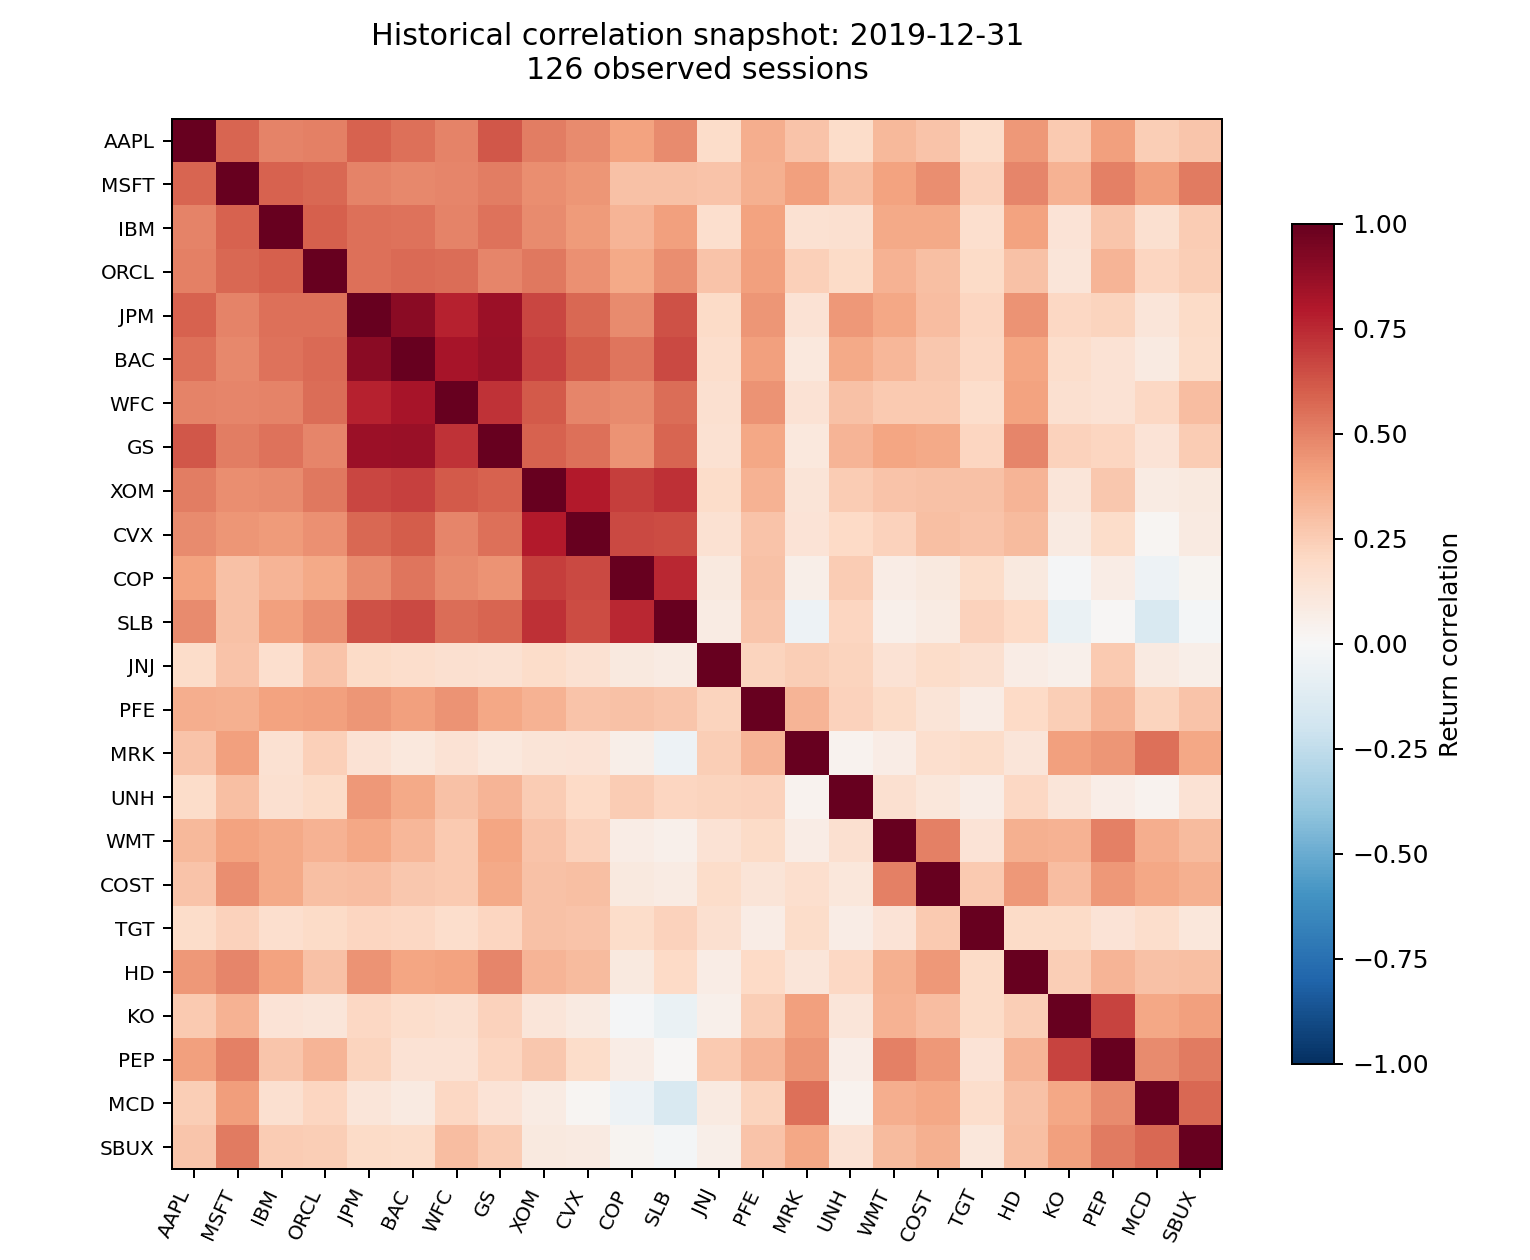
\includegraphics[width=\linewidth,height=.65\textheight,keepaspectratio]{assets/figure-01.png}

\caption{Historical 126-session correlation matrix at the last validation date}\label{fig:1}

\end{figure}

\hyperref[fig:1]{Figure 1} gives a static view of the last validation snapshot. The companion \textbf{Historical-Correlation-Explorer.html} contains 120 monthly frames, with rotation, zoom, a date slider and playback. Each frame uses trailing observations through the displayed date; no final-holdout data enter the surface.


The surface height is correlation, not expected return. Asset order remains fixed and the asset axes are discrete. The mesh joins neighbouring cells only for display, so values between stock labels should not be interpreted as estimated relationships between intermediate assets. The full correlation matrix is also distinct from the thresholded neighbour graph used by the strategy.


\bodyheading{Execution timing and portfolio accounting}

The accounting convention is deliberately explicit: a close-t observation produces a decision, the decision trades at close t+1, and the newly formed position first earns the return ending at close t+2. This is a modelling convention chosen to avoid obtaining a close price and simultaneously earning the return ending at that same close. It remains an approximation to executable orders.


\sourcemeta{Source: \textbf{market\_neutral/historical.py}, function \textbf{phase\_inputs}. Selected executable lines; surrounding input checks remain in the module.}

\par\addvspace{4pt}\noindent\begin{minipage}{\linewidth}

\begin{Verbatim}[fontsize=\small,baselinestretch=1.0,breaklines=true,breakanywhere=true,breakautoindent=true,breakindent=10pt,frame=single,framerule=.3pt,rulecolor=\color{tablerule},framesep=6pt,numbersep=5pt,numbers=left,xleftmargin=15pt,formatcom=\color{black}]
execution = weights.shift(1, fill_value=0.)
exposure = betas.shift(1)
mask = (returns.index >= pd.Timestamp(start)) & (returns.index <= pd.Timestamp(end))
\end{Verbatim}

\listingcaption{3}{Delaying decisions before slicing the evaluation phase}

\end{minipage}\par\addvspace{4pt}

\hyperref[lst:3]{Listing 3} shows why the shift occurs before period slicing. The first execution in a phase may use the preceding session's valid decision, but each phase begins with a flat book and fresh capital. The final close liquidates positions. Thus neither entry costs nor terminal closing costs disappear at an evaluation boundary.


\paperequation{10}{Short-borrow accrual}{B_t=a\frac{\Delta_t}{365}\sum_i\max(-v_{i,t-1},0)}

\hyperref[eq:10]{Equation 10} charges the annual rate a on the prior close's absolute short notional v. Delta counts elapsed calendar days, including weekends. This uniform borrow assumption is illustrative; it is not a historical security-level borrow series.


\paperequation{11}{Post-cost NAV and drift-aware trading cost}{V_t^{\mathrm{after}}+c\sum_i|w_{i,t}V_t^{\mathrm{after}}-v_{i,t}^{\mathrm{marked}}|=V_t^{\mathrm{before}}}

\hyperref[eq:11]{Equation 11} solves for NAV after trading fees. Where: c is the per-dollar fee and marked notionals incorporate the day's price changes. NAV before trading already reflects P\&L and borrow. The scalar solve makes target weights refer to equity after fees, avoiding a small exposure overshoot caused solely by transaction costs.


\paperequation{12}{Net-return reconciliation}{R_t^{\mathrm{net}}=\frac{\mathrm{PnL}_t-C_t-B_t}{V_{t-1}^{\mathrm{after}}}}

\hyperref[eq:12]{Equation 12} reconciles gross position P\&L, trading cost C and borrow cost B to net return. Turnover counts every dollar bought and every dollar sold, divided by start-of-day NAV. Cash interest, financing rebates, margin constraints and nonlinear market impact are not included.


\sourcemeta{Source: \textbf{market\_neutral/backtest.py}, function \textbf{execute\_targets}. Selected executable lines; surrounding input checks remain in the module.}

\par\addvspace{4pt}\noindent\begin{minipage}{\linewidth}

\begin{Verbatim}[fontsize=\small,baselinestretch=1.0,breaklines=true,breakanywhere=true,breakautoindent=true,breakindent=10pt,frame=single,framerule=.3pt,rulecolor=\color{tablerule},framesep=6pt,numbersep=5pt,numbers=left,xleftmargin=15pt,formatcom=\color{black}]
def balance(after):
    return after + cost_rate * np.abs(w * after - marked).sum() - nav_before_trade
if balance(0) >= 0:
    raise ValueError("Cannot fund trading costs")
nav = float(brentq(balance, 0, nav_before_trade, xtol=1e-10)) if cost_rate else nav_before_trade
\end{Verbatim}

\listingcaption{4}{Solving for equity after transaction costs}

\end{minipage}\par\addvspace{4pt}

\bodyheading{Historical baseline results}

\begingroup
\setcounter{table}{6}
\setstretch{1}\fontsize{10}{12.5}\selectfont
\renewcommand{\arraystretch}{1.12}
\arrayrulecolor{tablerule}
\begin{table}[!htbp]
\centering
\setstretch{1}\fontsize{10}{12.5}\selectfont
\begin{tabular}{P{0.490000\dimexpr\textwidth-6\tabcolsep\relax}Q{0.255000\dimexpr\textwidth-6\tabcolsep\relax}Q{0.255000\dimexpr\textwidth-6\tabcolsep\relax}}
\toprule
\rowcolor{tablehead} \textbf{Metric} & \textbf{Development} & \textbf{Validation} \\ \midrule
Total net return & -19.79\% & -16.44\% \\
\midrule[0.2pt]
Annualised net return & -3.10\% & -5.83\% \\
\midrule[0.2pt]
Annualised volatility & 3.17\% & 3.35\% \\
\midrule[0.2pt]
Zero-cash-rate Sharpe & -0.98 & -1.78 \\
\midrule[0.2pt]
Maximum drawdown & -24.99\% & -18.49\% \\
\midrule[0.2pt]
Realised SPY beta & 0.0202 & 0.0169 \\
\midrule[0.2pt]
Mean daily turnover & 41.00\% & 39.62\% \\
\midrule[0.2pt]
Mean gross exposure & 62.78\% & 61.29\% \\
\midrule[0.2pt]
Maximum absolute dollar exposure & 2.41e-15 & 3.52e-15 \\
\midrule[0.2pt]
Maximum absolute estimated beta & 2.29e-15 & 3.39e-15 \\
\bottomrule
\end{tabular}
\caption{Baseline performance at 5 bps and 2\% annual short borrow}\label{tab:7}
\end{table}
\endgroup

\hyperref[tab:7]{Table 7} reports a negative annualised return in both phases: -3.10\% in development and -5.83\% in validation. The numerical exposure constraints are satisfied, but these constraints do not imply a viable strategy. The practical issue is whether the signal can earn enough before costs to support its turnover.


Lo (2002), in \textit{The Statistics of Sharpe Ratios}, explains why return dependence and estimation error affect Sharpe-ratio interpretation. The statistic below uses the conventional square-root-of-time scaling and a zero cash rate for descriptive comparison. It is not a dependence-adjusted significance test or a confidence interval.


\paperequation{13}{Descriptive annualised Sharpe statistic}{\widehat{S}=\sqrt{252}\,\frac{\overline{R^{\mathrm{net}}}}{s(R^{\mathrm{net}})}}

\hyperref[eq:13]{Equation 13} uses the sample daily standard deviation. It is labelled as a zero-cash-rate statistic because cash interest is not modelled. Comparisons with an external fund's published Sharpe would require matching return and financing conventions.


\paperequation{14}{Drawdown from the running capital peak}{DD_t=\frac{V_t}{\max(V_0,V_1,\ldots,V_t)}-1}

\hyperref[eq:14]{Equation 14} includes initial capital in the running peak, so an early loss is counted. The reported maximum drawdown is the most negative observed value, including the final liquidation date.


\Needspace{4\baselineskip}\subsection{Capital paths and cost sensitivity}

\begin{figure}[!htbp]

\centering

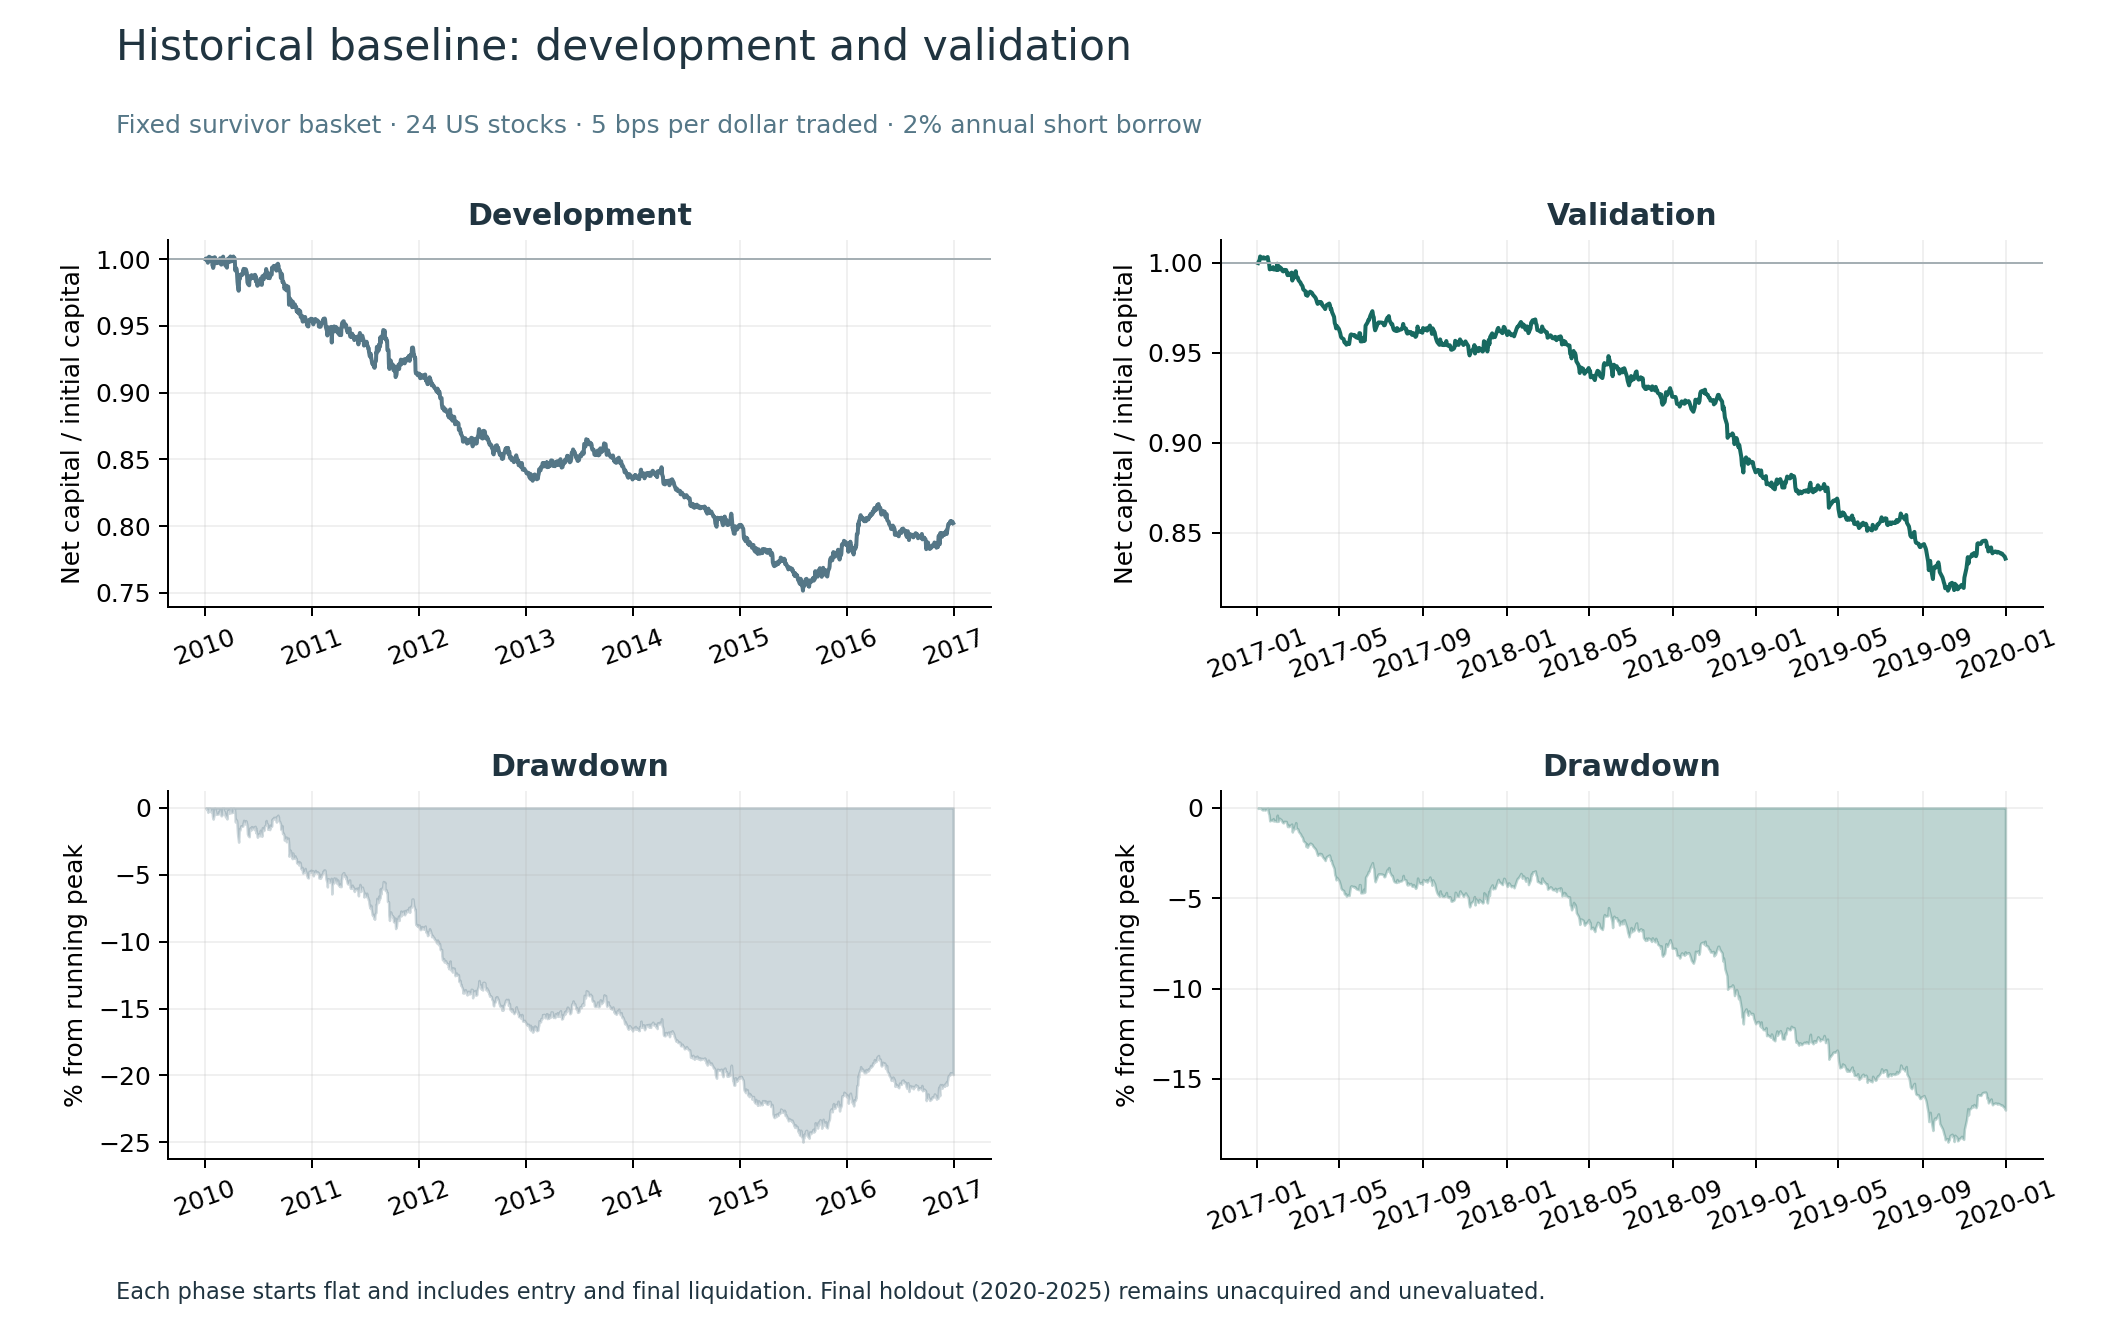
\includegraphics[width=\linewidth,height=.65\textheight,keepaspectratio]{assets/figure-02.png}

\caption{Baseline capital and drawdown; the holdout annotation records Milestone 2}\label{fig:2}

\end{figure}

\begingroup
\setcounter{table}{7}
\setstretch{1}\fontsize{10}{12.5}\selectfont
\renewcommand{\arraystretch}{1.12}
\arrayrulecolor{tablerule}
\begin{table}[!htbp]
\centering
\setstretch{1}\fontsize{10}{12.5}\selectfont
\begin{tabular}{P{0.240000\dimexpr\textwidth-6\tabcolsep\relax}Q{0.380000\dimexpr\textwidth-6\tabcolsep\relax}Q{0.380000\dimexpr\textwidth-6\tabcolsep\relax}}
\toprule
\rowcolor{tablehead} \textbf{Cost per dollar} & \textbf{Development CAGR} & \textbf{Validation CAGR} \\ \midrule
0 bps & 2.03\% & -1.00\% \\
\midrule[0.2pt]
5 bps & -3.10\% & -5.83\% \\
\midrule[0.2pt]
10 bps & -7.98\% & -10.41\% \\
\midrule[0.2pt]
20 bps & -17.02\% & -18.93\% \\
\bottomrule
\end{tabular}
\caption{All predeclared trading-cost scenarios; short borrow remains 2\%}\label{tab:8}
\end{table}
\endgroup

The zero-trading-fee scenario is not a costless portfolio: it still pays short borrow. Development is positive under that scenario, whereas validation is negative. Consequently, the validation failure cannot be attributed only to the 5 bps trading-fee assumption. The signal itself requires a stronger empirical comparison.


\Needspace{4\baselineskip}\subsection{Interpretation and remaining uncertainty}

\begin{figure}[!htbp]

\centering

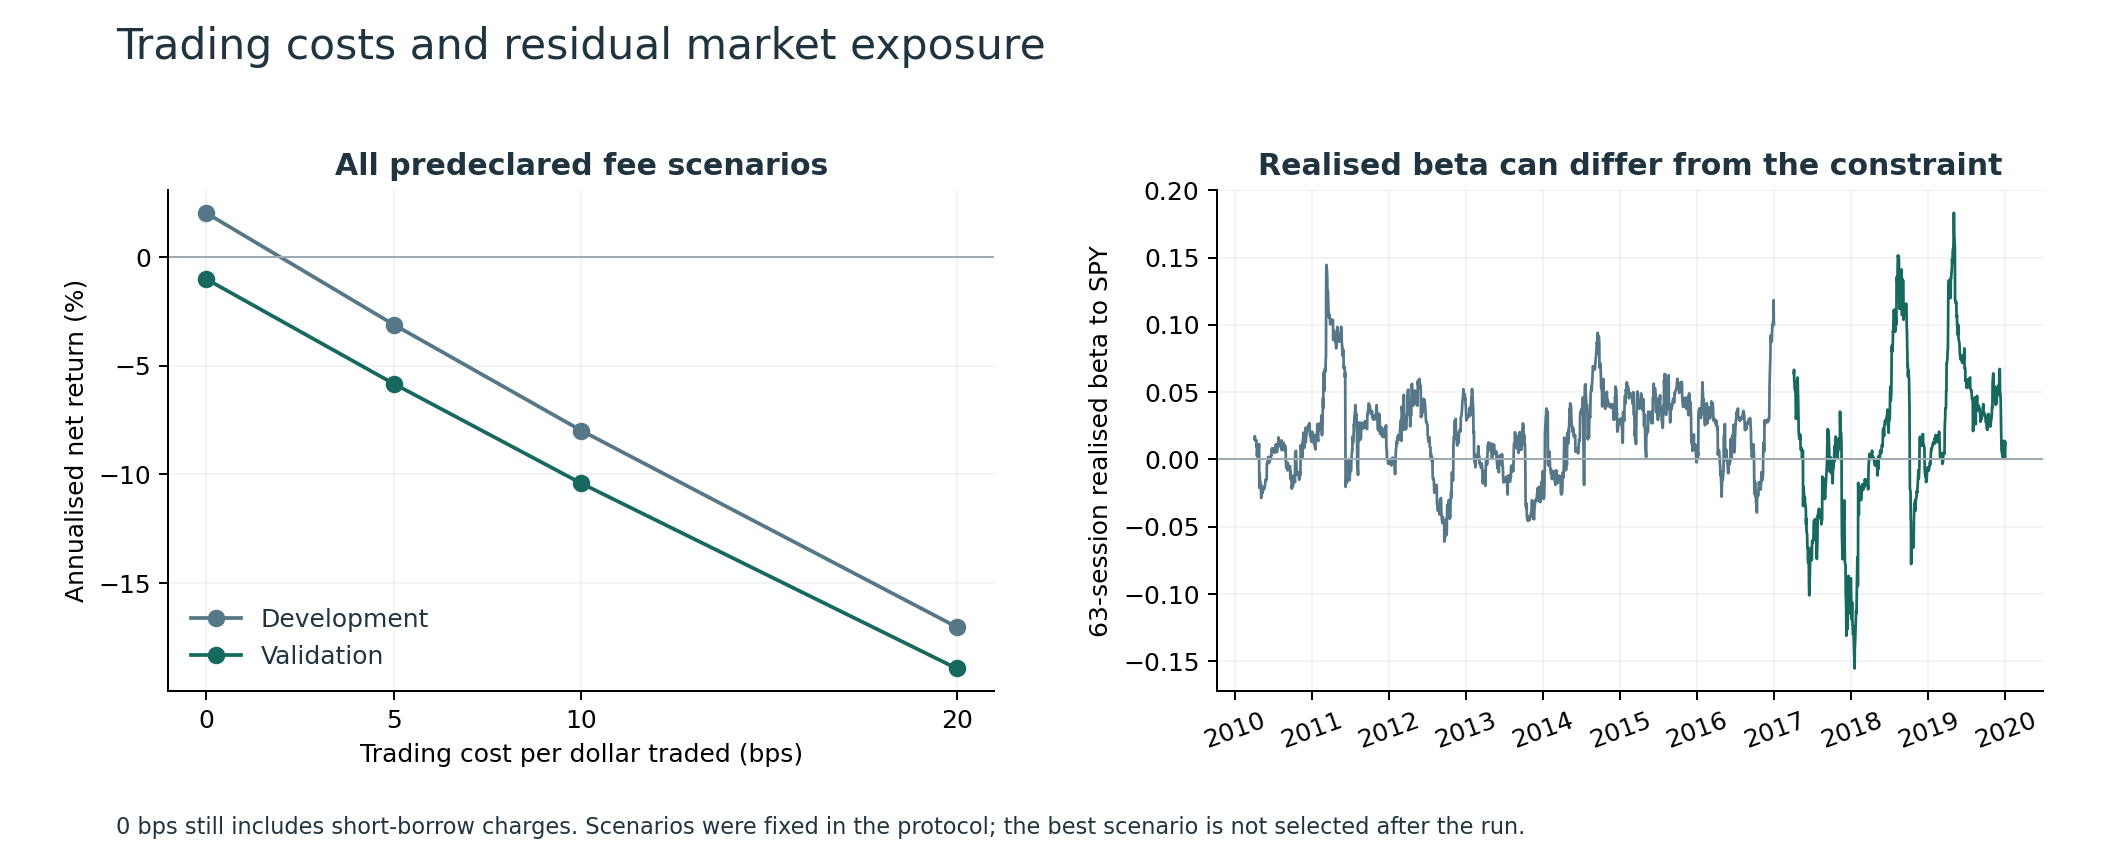
\includegraphics[width=\linewidth,height=.65\textheight,keepaspectratio]{assets/figure-03.png}

\caption{Sensitivity to trading costs and rolling realised market beta}\label{fig:3}

\end{figure}

\hyperref[fig:3]{Figure 3} demonstrates two separate issues. Net returns decline as the stated cost per dollar increases. Realised beta also varies through time despite the target constraint. The variation reflects an estimated hedge, a finite rolling measurement window and changing returns; it is not a contradiction of the recorded numerical neutrality checks.


Bailey et al. (2017), in \textit{The probability of backtest overfitting}, emphasise that a held-out sample alone does not account for repeated strategy searches. For this reason, the project records each experiment and does not interpret its chronological split as proof against overfitting. No PBO estimate, CSCV analysis or White reality-check statistic is calculated in this study.


The comparison in Section 8 retains these dates, costs, exposure ceilings and execution rules, including the unfavourable results. This requirement was carried into the final protocol in Section 10; no alternative was promoted after the final observations were inspected.


\bodyheading{Historical graph comparison}

Milestone 3 evaluates the graph rule in \hyperref[eq:9]{Equation 9} using exactly the acquired observations and accounting conventions from the historical baseline. The baseline outcome was known when this comparison began. The graph settings were inherited from the synthetic prototype, and a separate local protocol was hashed before the first historical graph run. Neither development nor validation is represented as a newly untouched dataset.


\begingroup
\setcounter{table}{8}
\setstretch{1}\fontsize{10}{12.5}\selectfont
\renewcommand{\arraystretch}{1.12}
\arrayrulecolor{tablerule}
\begin{table}[!htbp]
\centering
\setstretch{1}\fontsize{10}{12.5}\selectfont
\begin{tabular}{P{0.280000\dimexpr\textwidth-4\tabcolsep\relax}P{0.720000\dimexpr\textwidth-4\tabcolsep\relax}}
\toprule
\rowcolor{tablehead} \textbf{Component} & \textbf{Fixed design} \\ \midrule
Primary candidate & 126-session graph; five directed neighbours above 0.20; symmetric union; diffusion time one \\
\midrule[0.2pt]
Trading-fee sensitivity & 0, 5, 10 and 20 bps; 2\% annual borrow \\
\midrule[0.2pt]
Diffusion-time sensitivity & 0.5, 1 and 2; every trading-fee combination retained \\
\midrule[0.2pt]
Borrow sensitivity & 0\%, 2\% and 5\%; baseline and primary graph at 5 bps \\
\midrule[0.2pt]
Exposure control & Both primary targets scaled down to their common daily gross exposure; 5 bps and 2\% borrow \\
\midrule[0.2pt]
Uncertainty & Paired stationary bootstrap, 5,000 replicates; mean block lengths 5/10/20; HAC with 10 lags \\
\midrule[0.2pt]
Experiment record & 44 distinct backtests completed; no replacement of the primary candidate \\
\midrule[0.2pt]
Holdout at Milestone 3 & 2020–2025 was unacquired; Section 10 records its later release \\
\bottomrule
\end{tabular}
\caption{Predeclared comparison and sensitivity design}\label{tab:9}
\end{table}
\endgroup

As White (2000) argues in \textit{A Reality Check for Data Snooping}, searching across alternatives can produce misleading apparent success. For this reason, all declared sensitivity results are retained and the primary candidate remains tau = 1. This protocol does not implement White's multiple-comparison test or retrospectively remove earlier knowledge of the baseline.


\sourcemeta{Source: \textbf{market\_neutral/strategy.py}, function \textbf{build\_decisions}. Selected executable lines; surrounding input checks remain in the module.}

\par\addvspace{4pt}\noindent\begin{minipage}{\linewidth}

\begin{Verbatim}[fontsize=\small,baselinestretch=1.0,breaklines=true,breakanywhere=true,breakautoindent=true,breakindent=10pt,frame=single,framerule=.3pt,rulecolor=\color{tablerule},framesep=6pt,numbersep=5pt,numbers=left,xleftmargin=15pt,formatcom=\color{black}]
corr, adjacency, laplacian = correlation_graph(
    r[t + 1 - config.correlation_window:t + 1],
    config.neighbours, config.minimum_correlation)
smooth = heat_diffusion(shock, laplacian, config.diffusion_time)
scores = {"baseline": -shock, "graph": -(shock - smooth)}
\end{Verbatim}

\listingcaption{5}{Constructing the graph-relative score from the same observed shock}

\end{minipage}\par\addvspace{4pt}

\Needspace{4\baselineskip}\subsection{Primary historical outcomes}

\begingroup
\setcounter{table}{9}
\setstretch{1}\fontsize{10}{12.5}\selectfont
\renewcommand{\arraystretch}{1.12}
\arrayrulecolor{tablerule}
\begin{table}[!htbp]
\centering
\setstretch{1}\fontsize{10}{12.5}\selectfont
\begin{tabular}{P{0.280000\dimexpr\textwidth-12\tabcolsep\relax}Q{0.145000\dimexpr\textwidth-12\tabcolsep\relax}Q{0.145000\dimexpr\textwidth-12\tabcolsep\relax}Q{0.150000\dimexpr\textwidth-12\tabcolsep\relax}Q{0.140000\dimexpr\textwidth-12\tabcolsep\relax}Q{0.140000\dimexpr\textwidth-12\tabcolsep\relax}}
\toprule
\rowcolor{tablehead} \textbf{Phase / model} & \textbf{Ann. net return} & \textbf{Ann. volatility} & \textbf{Max. drawdown} & \textbf{Mean gross} & \textbf{Mean turnover} \\ \midrule
Development / Baseline & -3.10\% & 3.17\% & -24.99\% & 62.78\% & 41.00\% \\
\midrule[0.2pt]
Development / Graph, tau = 1 & -4.37\% & 2.89\% & -27.97\% & 62.18\% & 40.44\% \\
\midrule[0.2pt]
Validation / Baseline & -5.83\% & 3.35\% & -18.49\% & 61.29\% & 39.62\% \\
\midrule[0.2pt]
Validation / Graph, tau = 1 & -5.27\% & 2.92\% & -16.20\% & 60.63\% & 39.73\% \\
\bottomrule
\end{tabular}
\caption{Primary strategies at 5 bps trading fees and 2\% borrow}\label{tab:10}
\end{table}
\endgroup

The graph candidate earns -4.37\% annualised in development, compared with -3.10\% for the baseline. In validation, the corresponding values are -5.27\% and -5.83\%. The graph-minus-baseline CAGR differences are therefore -1.26 and +0.55 percentage points. Both strategies lose money at the default costs.


\begin{figure}[!htbp]

\centering

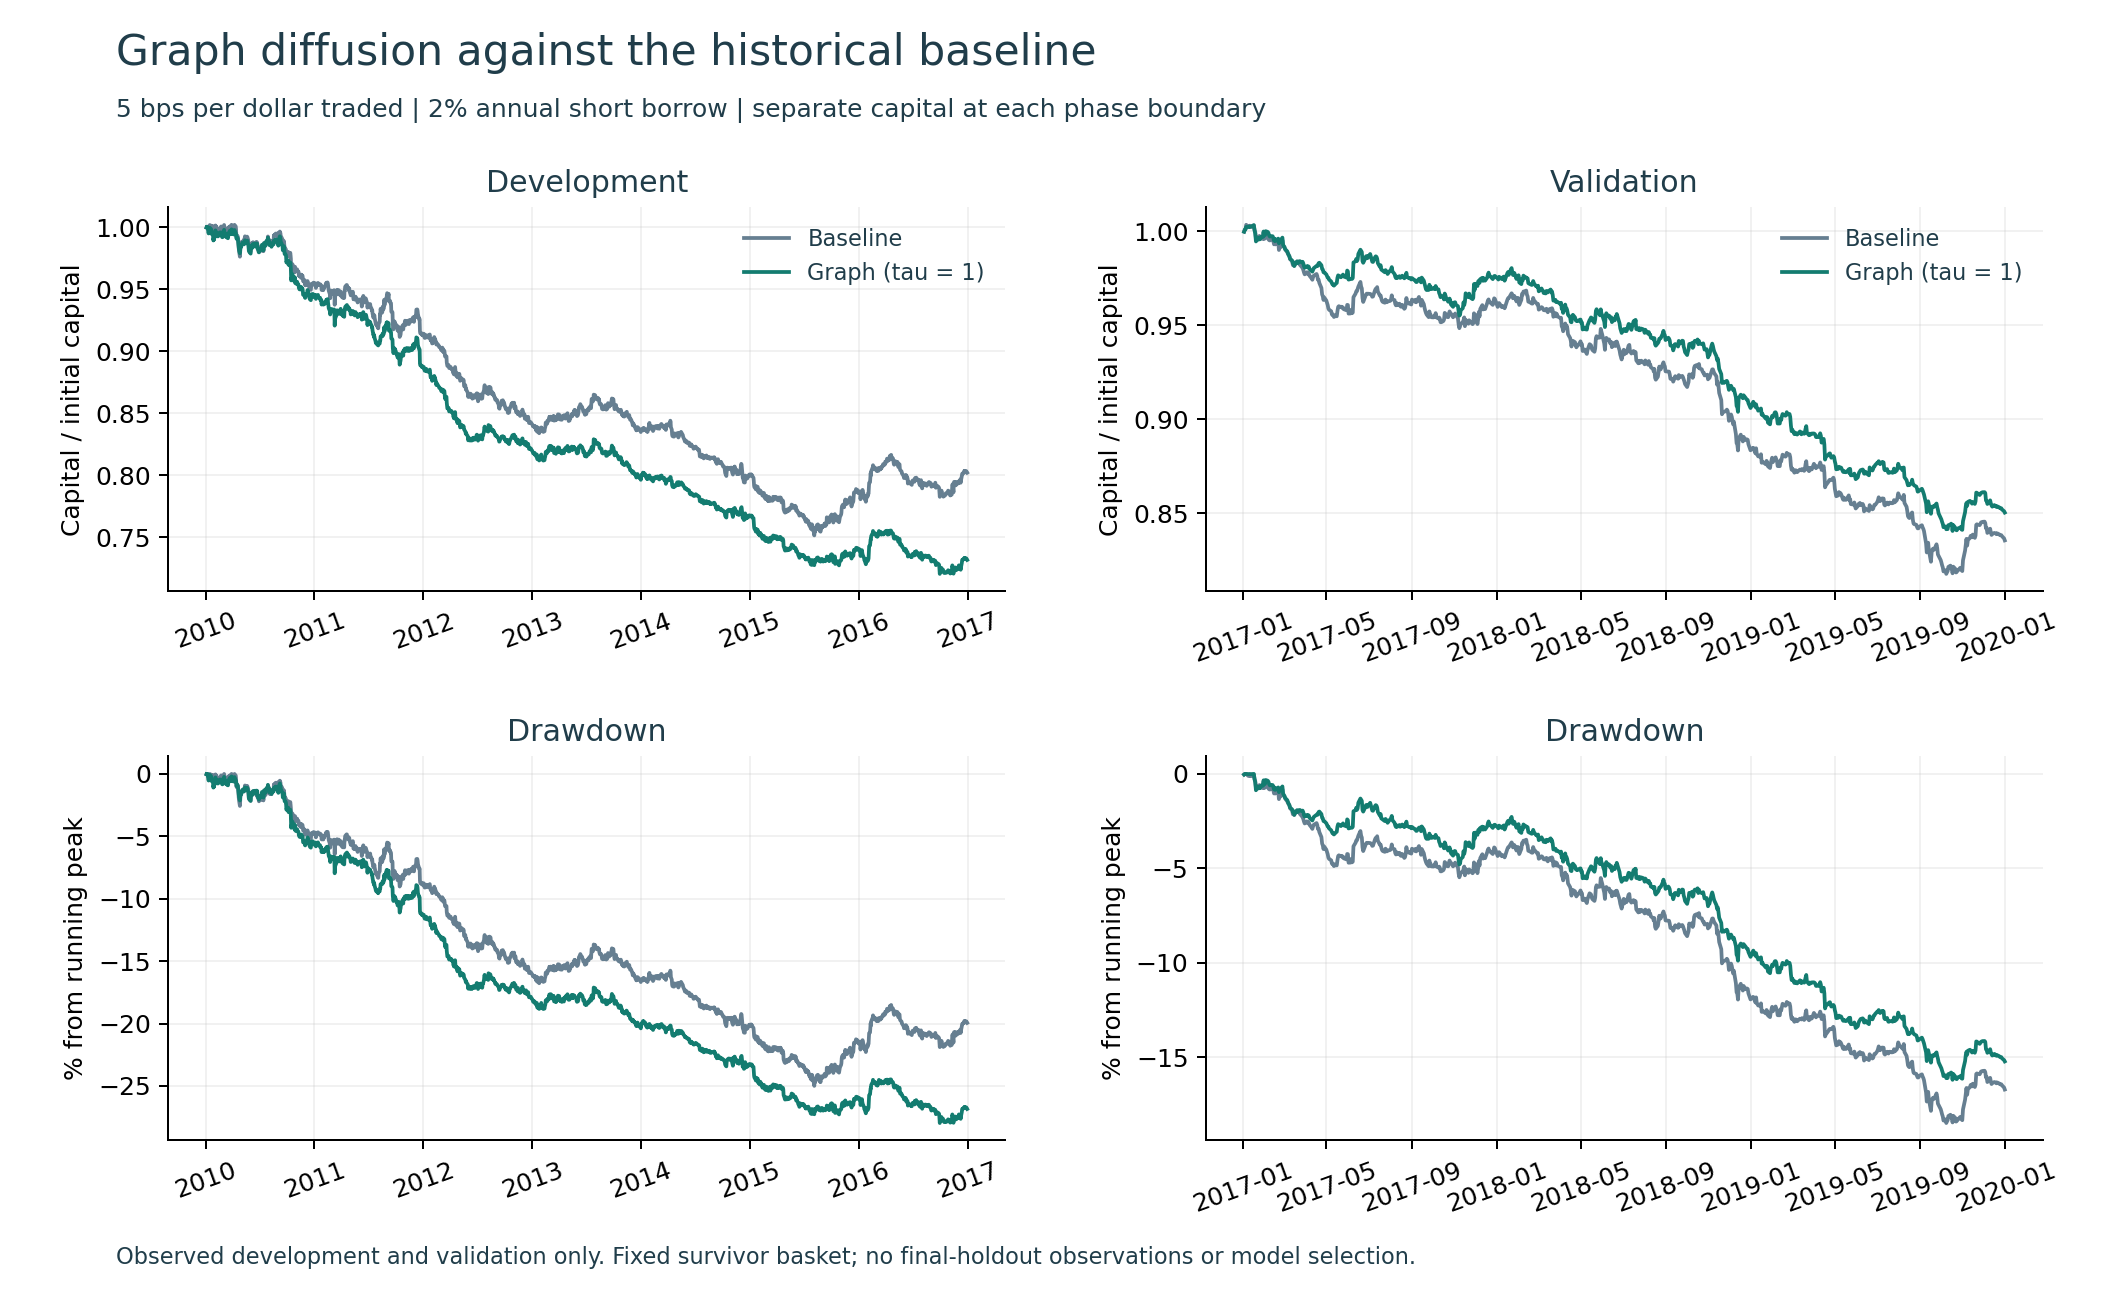
\includegraphics[width=\linewidth,height=.65\textheight,keepaspectratio]{assets/figure-04.png}

\caption{Baseline and graph capital paths under identical accounting conventions}\label{fig:4}

\end{figure}

The graph portfolio has somewhat lower realised volatility and lower mean gross exposure. Equal exposure ceilings do not force equal realised capital utilisation. Therefore, the return comparison alone cannot isolate the effect of the graph signal from the portfolio scaling that follows it.


\Needspace{4\baselineskip}\subsection{A causal control for gross exposure}

The control below matches the two portfolios at the decision close. It reduces both targets to the smaller of their gross exposures, then applies the original execution delay. It does not scale a portfolio upward, use realised future volatility or relax a name limit. This is a project-specific diagnostic, not a claim that equal gross exposure implies equal risk.


\paperequation{15}{Matching the gross exposure of the two decision portfolios}{G_t^*=\min(\|w_t^B\|_1,\|w_t^G\|_1),\qquad w_t^{j,*}=w_t^j\frac{G_t^*}{\|w_t^j\|_1}}

\hyperref[eq:15]{Equation 15} defines the control for j equal to baseline B or graph G. A zero denominator gives a flat vector. Uniform shrinking preserves dollar and estimated-beta neutrality and cannot increase any absolute name weight. Risk and sector composition can still differ.


\sourcemeta{Source: \textbf{market\_neutral/comparison.py}, function \textbf{match\_gross\_exposure}. Selected executable lines; surrounding input checks remain in the module.}

\par\addvspace{4pt}\noindent\begin{minipage}{\linewidth}

\begin{Verbatim}[fontsize=\small,baselinestretch=1.0,breaklines=true,breakanywhere=true,breakautoindent=true,breakindent=10pt,frame=single,framerule=.3pt,rulecolor=\color{tablerule},framesep=6pt,numbersep=5pt,numbers=left,xleftmargin=15pt,formatcom=\color{black}]
gross_baseline = baseline.abs().sum(axis=1)
gross_graph = graph.abs().sum(axis=1)
common = np.minimum(gross_baseline, gross_graph)
controls = []
for weights, gross in [(baseline, gross_baseline), (graph, gross_graph)]:
    factor = common.div(gross.where(gross > 1e-14)).fillna(0.)
    controls.append(weights.mul(factor, axis=0))
\end{Verbatim}

\listingcaption{6}{Matching exposure without levering either portfolio upward}

\end{minipage}\par\addvspace{4pt}

\begingroup
\setcounter{table}{10}
\setstretch{1}\fontsize{10}{12.5}\selectfont
\renewcommand{\arraystretch}{1.12}
\arrayrulecolor{tablerule}
\begin{table}[!htbp]
\centering
\setstretch{1}\fontsize{10}{12.5}\selectfont
\begin{tabular}{P{0.220000\dimexpr\textwidth-10\tabcolsep\relax}Q{0.185000\dimexpr\textwidth-10\tabcolsep\relax}Q{0.185000\dimexpr\textwidth-10\tabcolsep\relax}Q{0.200000\dimexpr\textwidth-10\tabcolsep\relax}Q{0.210000\dimexpr\textwidth-10\tabcolsep\relax}}
\toprule
\rowcolor{tablehead} \textbf{Phase} & \textbf{Baseline CAGR} & \textbf{Graph CAGR} & \textbf{Difference (pp)} & \textbf{Common mean gross} \\ \midrule
Development & -3.03\% & -4.05\% & -1.03 & 57.65\% \\
\midrule[0.2pt]
Validation & -5.16\% & -4.95\% & +0.22 & 56.38\% \\
\bottomrule
\end{tabular}
\caption{Separate backtests of the matched-gross controls}\label{tab:11}
\end{table}
\endgroup

The validation advantage becomes smaller when gross exposure is matched, while the development disadvantage remains. This reinforces the need to discuss exposure and volatility alongside return. The controls are fully rerun portfolios, not an after-the-fact division of the original returns by average exposure.


\Needspace{4\baselineskip}\subsection{Paired uncertainty with dependent observations}

The uncertainty calculation concerns the paired daily net-return difference at the primary cost settings. Both strategies experience the same dates and market observations. Resampling their paired difference preserves that contemporaneous comparison; resampling the two strategies independently would discard it.


\paperequation{16}{Paired daily difference and annualised arithmetic mean}{\delta_t=R_t^{G,\mathrm{net}}-R_t^{B,\mathrm{net}},\qquad \widehat{\mu}_{\mathrm{ann}}=252\,\bar\delta}

\hyperref[eq:16]{Equation 16} defines the estimated annualised arithmetic difference. It is not the difference between the two compounded annual growth rates. The uncertainty intervals below refer to this mean, so their estimate should not be substituted for the CAGR difference in the performance table.


Politis and Romano (1994) introduce the stationary bootstrap in \textit{The Stationary Bootstrap}. Nordman (2009) restates its geometric-block construction in Section 2.1 of \textit{A note on the stationary bootstrap's variance}. Following that construction, this implementation restarts at a uniformly chosen observed date or continues circularly from the preceding sampled index.


\paperequation{17}{Random restarts and circular continuation in the stationary bootstrap}{\Pr(\mathrm{restart})=\ell^{-1},\qquad I_{k+1}^*=1+(I_k^*\ \mathrm{mod}\ T)}

\hyperref[eq:17]{Equation 17} gives the restart probability and the continuation rule when no restart occurs. Here ell is the expected block length, T is the phase sample size and the mathematical indices run from 1 to T. On a restart, a new index is uniform on that range. Python uses the equivalent zero-based convention.


\sourcemeta{Source: \textbf{market\_neutral/inference.py}, function \textbf{stationary\_indices}. Selected executable lines; surrounding input checks remain in the module.}

\par\addvspace{4pt}\noindent\begin{minipage}{\linewidth}

\begin{Verbatim}[fontsize=\small,baselinestretch=1.0,breaklines=true,breakanywhere=true,breakautoindent=true,breakindent=10pt,frame=single,framerule=.3pt,rulecolor=\color{tablerule},framesep=6pt,numbersep=5pt,numbers=left,xleftmargin=15pt,formatcom=\color{black}]
indices = np.empty((replicates, observations), dtype=np.int32)
indices[:, 0] = rng.integers(0, observations, size=replicates)
for t in range(1, observations):
    restart = rng.random(replicates) < 1.0 / mean_block_length
    new_start = rng.integers(0, observations, size=replicates)
    indices[:, t] = np.where(restart, new_start, (indices[:, t - 1] + 1) % observations)
\end{Verbatim}

\listingcaption{7}{Preserving blocks through random restarts and circular continuation}

\end{minipage}\par\addvspace{4pt}

The primary interval uses 5,000 replicates and expected block length 10; lengths 5 and 20 are retained as sensitivity checks. The reported bounds are the 2.5th and 97.5th percentiles of the bootstrap mean, multiplied by 252. Seeds are specified in the protocol and derive deterministically from phase and block length. No block length is chosen because it yields a preferred conclusion.


\Needspace{4\baselineskip}\subsection{HAC cross-check and interpretation}

Newey and West (1987), in \textit{A Simple, Positive Semi-Definite, Heteroskedasticity and Autocorrelation Consistent Covariance Matrix}, develop a covariance estimator using weighted lagged covariances. Their 1986 working-paper version was consulted for the Bartlett weights. Here the intercept-only special case supplies a second estimate of uncertainty for the paired mean.


\paperequation{18}{Bartlett-weighted long-run variance of the paired difference}{\widehat{\Omega}=\widehat{\gamma}_0+2\sum_{k=1}^{K}\left(1-\frac{k}{K+1}\right)\widehat{\gamma}_k}

\hyperref[eq:18]{Equation 18} uses K = 10 lags. Each gamma-hat is the sum of products of mean-centred paired differences k observations apart, divided by the full phase length T. The same T denominator is used at every lag. This convention is checked against the equivalent Bartlett quadratic form.


\paperequation{19}{HAC standard error of the annualised arithmetic difference}{\widehat{\mathrm{SE}}(\widehat{\mu}_{\mathrm{ann}})=252\sqrt{\widehat{\Omega}/T}}

\hyperref[eq:19]{Equation 19} scales the standard error of the sample mean by 252. It does not use square-root-of-252 volatility scaling. The approximate 95\% HAC interval adds and subtracts the standard-normal critical value times this standard error.


\sourcemeta{Source: \textbf{market\_neutral/inference.py}, function \textbf{hac\_mean\_interval}. Selected executable lines; surrounding input checks remain in the module.}

\par\addvspace{4pt}\noindent\begin{minipage}{\linewidth}

\begin{Verbatim}[fontsize=\small,baselinestretch=1.0,breaklines=true,breakanywhere=true,breakautoindent=true,breakindent=10pt,frame=single,framerule=.3pt,rulecolor=\color{tablerule},framesep=6pt,numbersep=5pt,numbers=left,xleftmargin=15pt,formatcom=\color{black}]
centered = x - x.mean()
n = len(x)
long_run_variance = float(centered @ centered / n)
for lag in range(1, lags + 1):
    covariance = float(centered[lag:] @ centered[:-lag] / n)
    long_run_variance += 2 * (1 - lag / (lags + 1)) * covariance
\end{Verbatim}

\listingcaption{8}{Accumulating serial covariance with Bartlett weights}

\end{minipage}\par\addvspace{4pt}

\begingroup
\setcounter{table}{11}
\setstretch{1}\fontsize{10}{12.5}\selectfont
\renewcommand{\arraystretch}{1.12}
\arrayrulecolor{tablerule}
\begin{table}[!htbp]
\centering
\setstretch{1}\fontsize{10}{12.5}\selectfont
\begin{tabular}{P{0.190000\dimexpr\textwidth-8\tabcolsep\relax}Q{0.210000\dimexpr\textwidth-8\tabcolsep\relax}Q{0.300000\dimexpr\textwidth-8\tabcolsep\relax}Q{0.300000\dimexpr\textwidth-8\tabcolsep\relax}}
\toprule
\rowcolor{tablehead} \textbf{Phase} & \textbf{Mean difference (pp)} & \textbf{95\% bootstrap interval (pp)} & \textbf{95\% HAC interval (pp)} \\ \midrule
Development & -1.32 & [-2.18, -0.47] & [-2.15, -0.49] \\
\midrule[0.2pt]
Validation & +0.57 & [-1.16, +2.37] & [-1.16, +2.30] \\
\bottomrule
\end{tabular}
\caption{Pointwise uncertainty for the primary paired-return difference}\label{tab:12}
\end{table}
\endgroup

The development intervals lie below zero, while every validation interval spans zero. Thus the modest positive validation point estimate does not establish a reliable graph advantage. These are approximate, pointwise intervals conditional on the observed policies and basket. They assume adequate stationarity and weak dependence, do not refit signals on bootstrapped price paths, and cannot correct survivorship bias, historical selection or repeated model searching.


\Needspace{4\baselineskip}\subsection{Sensitivity and the economic effect of costs}

\begin{figure}[!htbp]

\centering

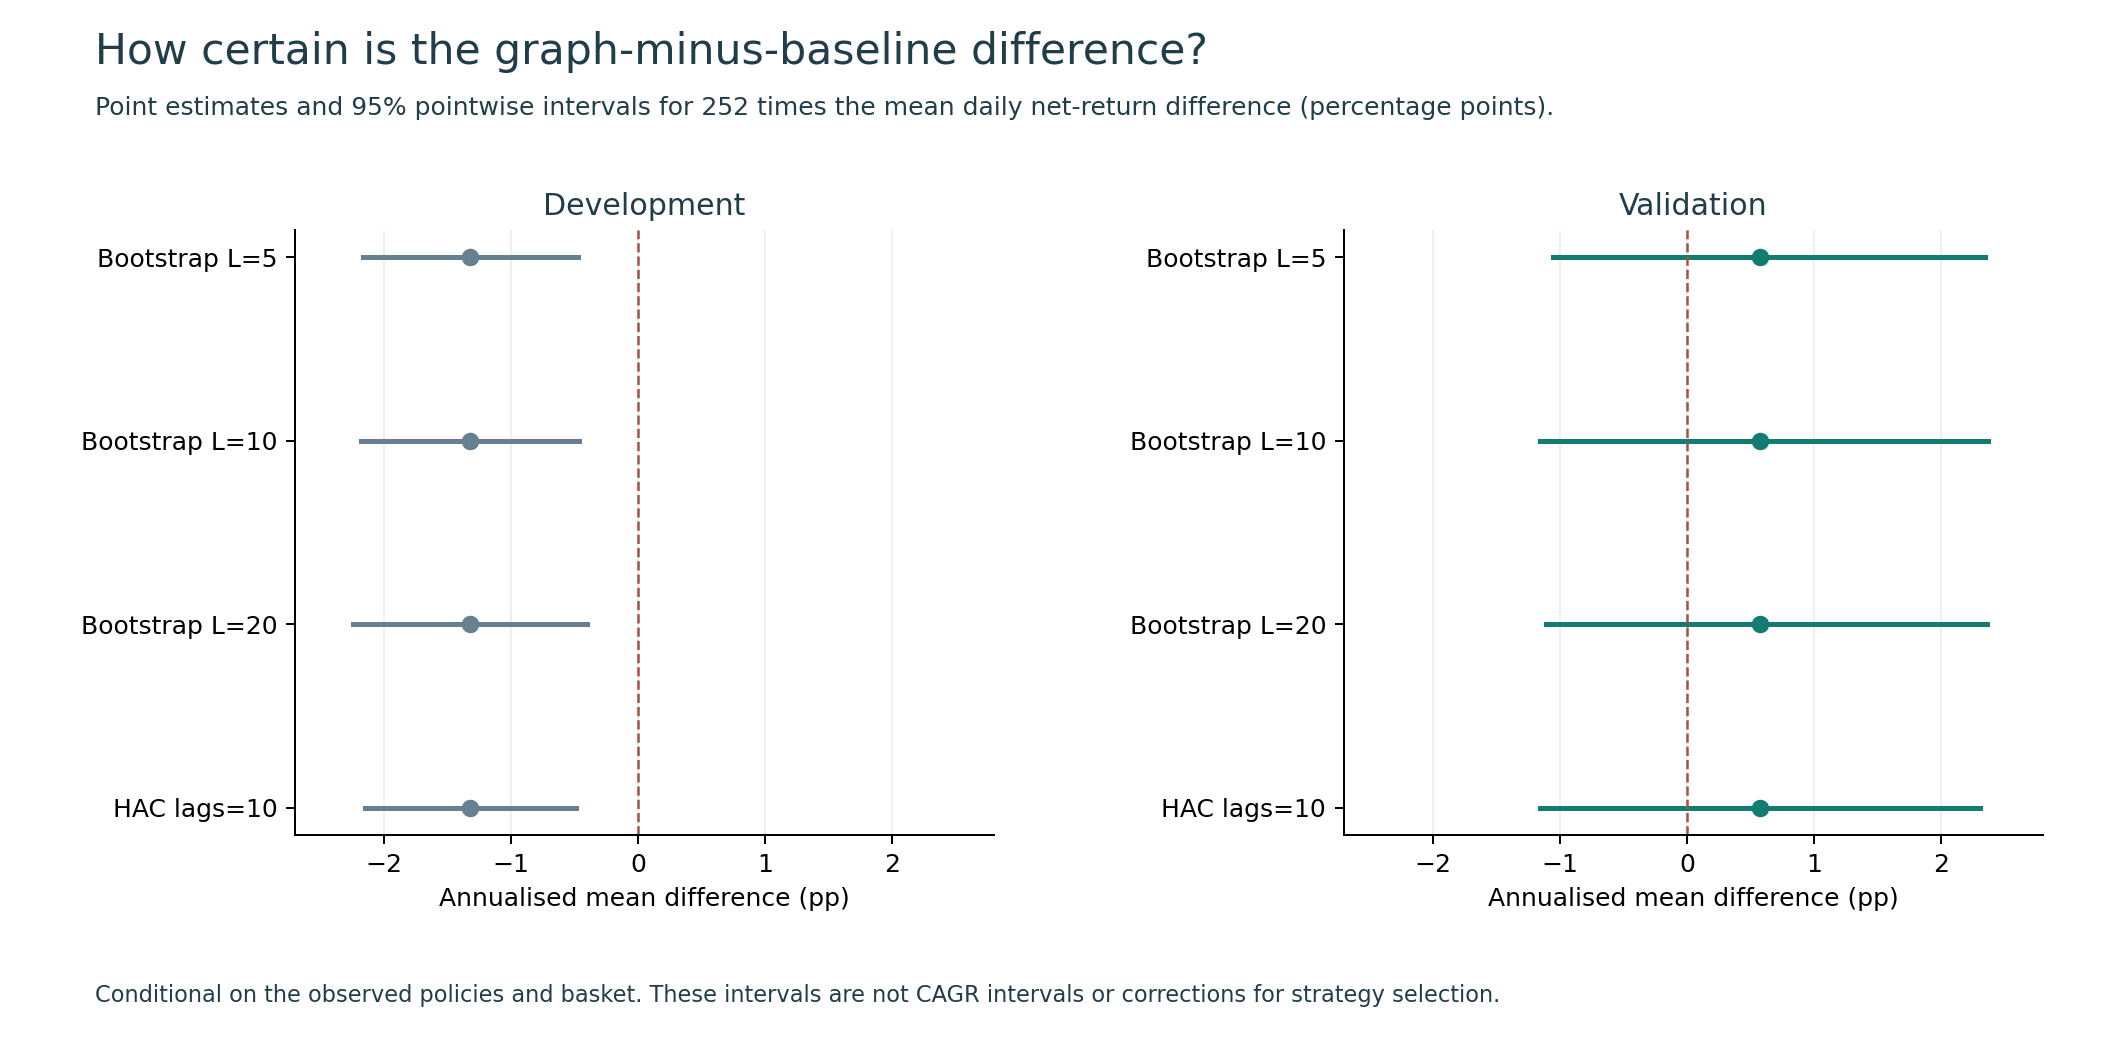
\includegraphics[width=\linewidth,height=.65\textheight,keepaspectratio]{assets/figure-05.png}

\caption{Stationary-bootstrap and HAC intervals for the paired mean}\label{fig:5}

\end{figure}

\begin{figure}[!htbp]

\centering

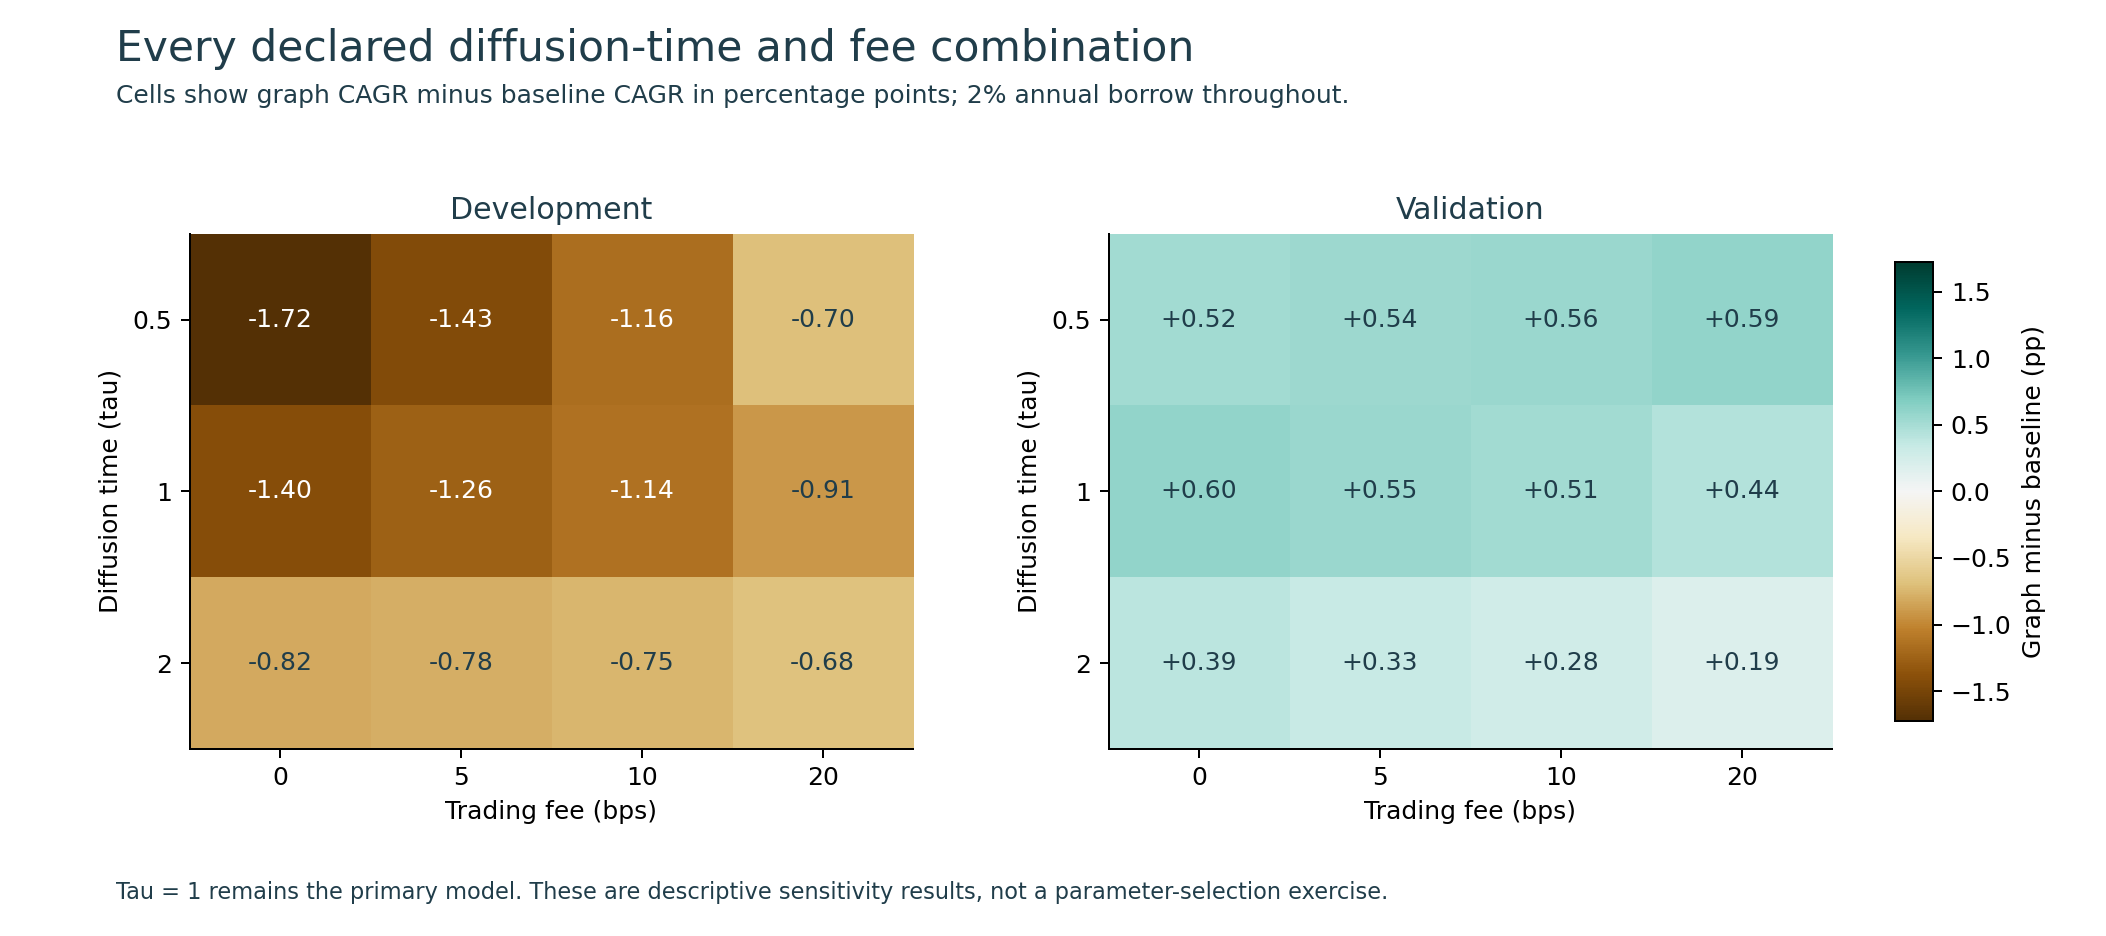
\includegraphics[width=\linewidth,height=.65\textheight,keepaspectratio]{assets/figure-06.png}

\caption{Graph-minus-baseline CAGR across every declared fee and diffusion time}\label{fig:6}

\end{figure}

Every tested diffusion time underperforms the baseline in development and improves its validation CAGR slightly. None is profitable in validation, even when trading fees are zero and borrow remains 2\%. This pattern is retained without promoting a different diffusion time to the primary specification. The complete scenario values and calendar-year returns are supplied as machine-readable outputs.


\Needspace{4\baselineskip}\subsection{Gross contribution, borrow and turnover}

\begin{figure}[!htbp]

\centering

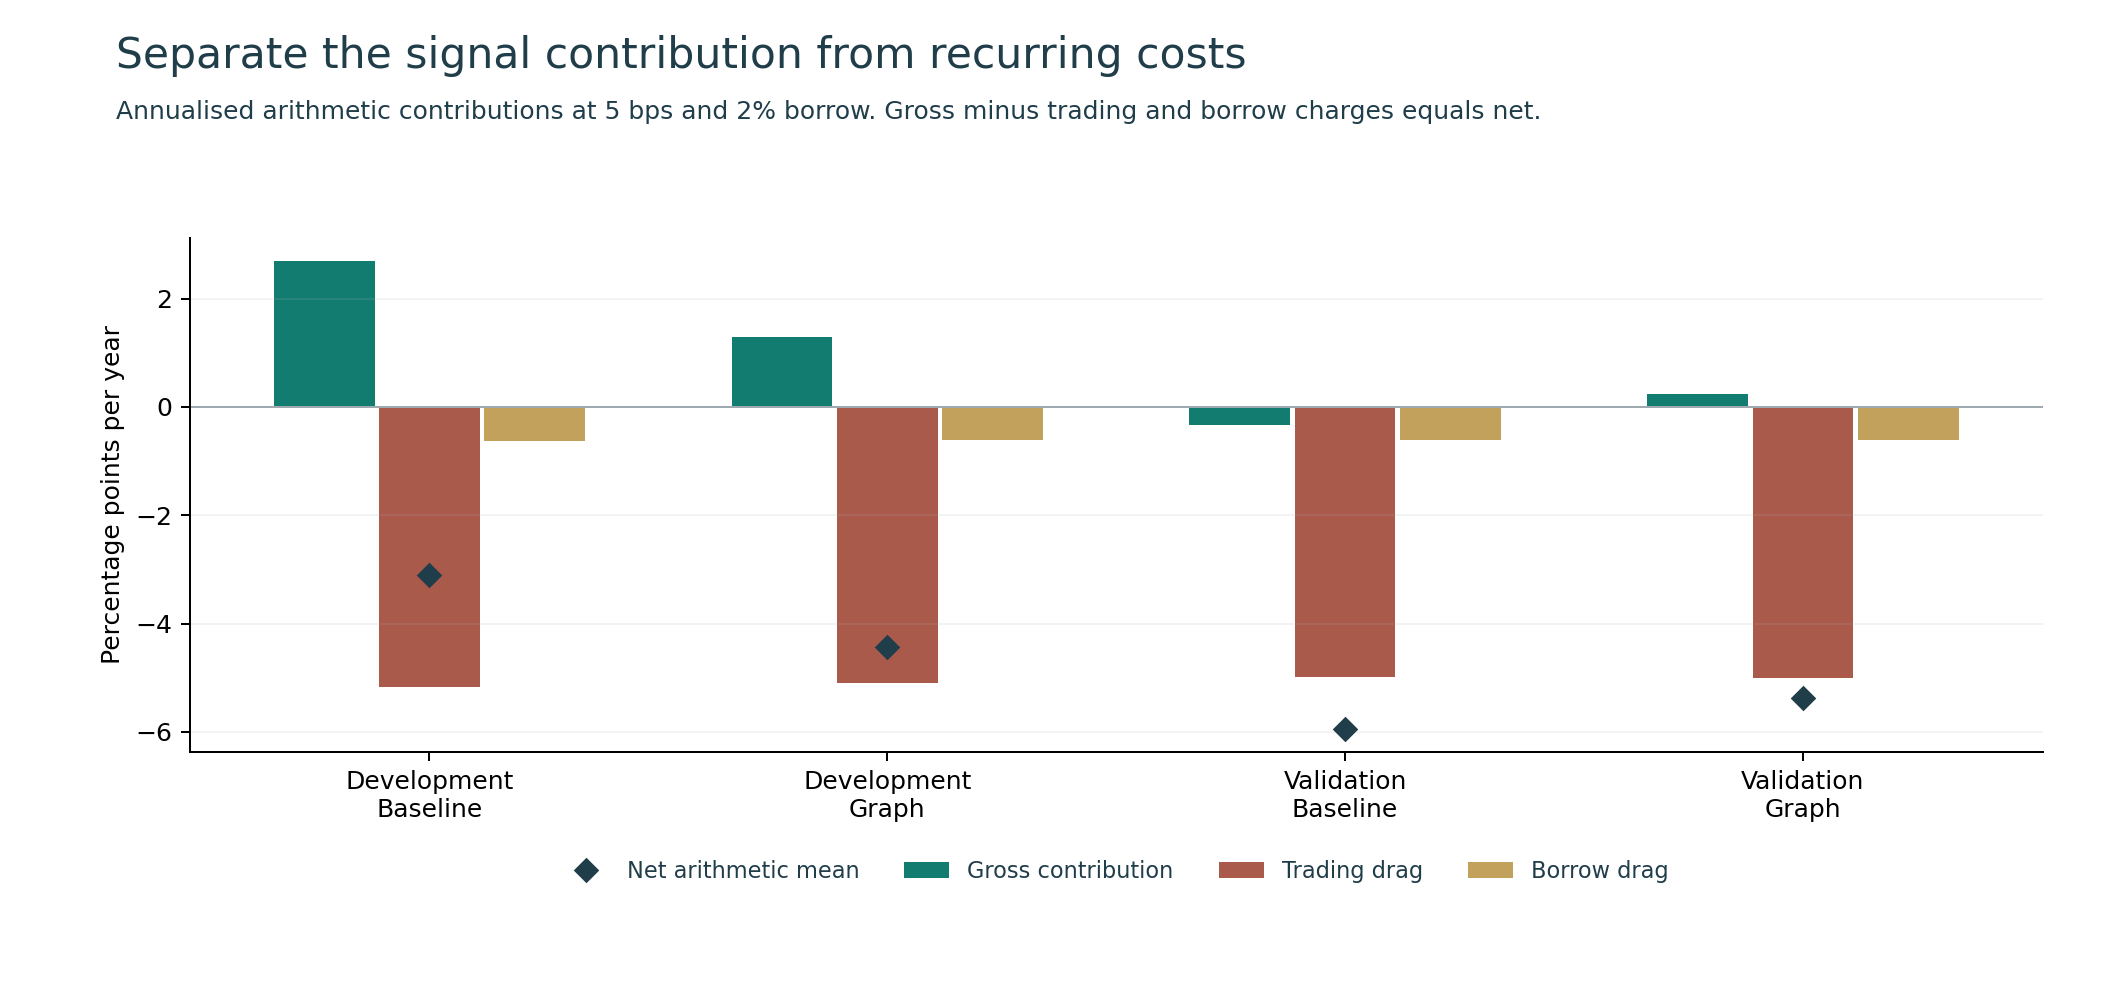
\includegraphics[width=\linewidth,height=.65\textheight,keepaspectratio]{assets/figure-07.png}

\caption{Annualised arithmetic return contributions and recurring charges}\label{fig:7}

\end{figure}

For the primary graph in development, the positive gross arithmetic contribution is insufficient to cover trading and borrowing charges. In validation its gross contribution is smaller still. This diagnosis is more informative than reporting a Sharpe statistic alone: the graph changes the relative allocation, but the observed gross signal does not finance the declared turnover cost.


\begingroup
\setcounter{table}{12}
\setstretch{1}\fontsize{10}{12.5}\selectfont
\renewcommand{\arraystretch}{1.12}
\arrayrulecolor{tablerule}
\begin{table}[!htbp]
\centering
\setstretch{1}\fontsize{10}{12.5}\selectfont
\begin{tabular}{P{0.220000\dimexpr\textwidth-10\tabcolsep\relax}Q{0.195000\dimexpr\textwidth-10\tabcolsep\relax}Q{0.195000\dimexpr\textwidth-10\tabcolsep\relax}Q{0.195000\dimexpr\textwidth-10\tabcolsep\relax}Q{0.195000\dimexpr\textwidth-10\tabcolsep\relax}}
\toprule
\rowcolor{tablehead} \textbf{Annual borrow} & \textbf{Dev. baseline} & \textbf{Dev. graph} & \textbf{Val. baseline} & \textbf{Val. graph} \\ \midrule
0\% & -2.49\% & -3.77\% & -5.25\% & -4.69\% \\
\midrule[0.2pt]
2\% & -3.10\% & -4.37\% & -5.83\% & -5.27\% \\
\midrule[0.2pt]
5\% & -4.01\% & -5.25\% & -6.69\% & -6.13\% \\
\bottomrule
\end{tabular}
\caption{Borrow sensitivity: CAGR with trading fees fixed at 5 bps}\label{tab:13}
\end{table}
\endgroup

The zero-borrow case retains transaction fees. It is a sensitivity scenario, not an assertion that every short can be financed for free. Likewise, a uniform 5\% borrow rate does not represent security-specific availability or a stressed lending book. These tests describe the assumed ledger, not executable brokerage terms.


\Needspace{4\baselineskip}\subsection{Interpreting diffusion through an interactive graph}

\paperequation{20}{Spectral gain applied to the unsmoothed residual}{g_{\tau}(\lambda)=1-\exp(-\tau\lambda)}

\hyperref[eq:20]{Equation 20} follows directly from \hyperref[eq:8]{Equation 8}: an eigenvector of L with eigenvalue lambda is multiplied by this factor in x minus its diffused value. The zero-eigenvalue component is removed. Changing tau changes the relative treatment of graph modes; the subsequent exposure projection and scaling remain separate operations.


\begin{figure}[!htbp]

\centering

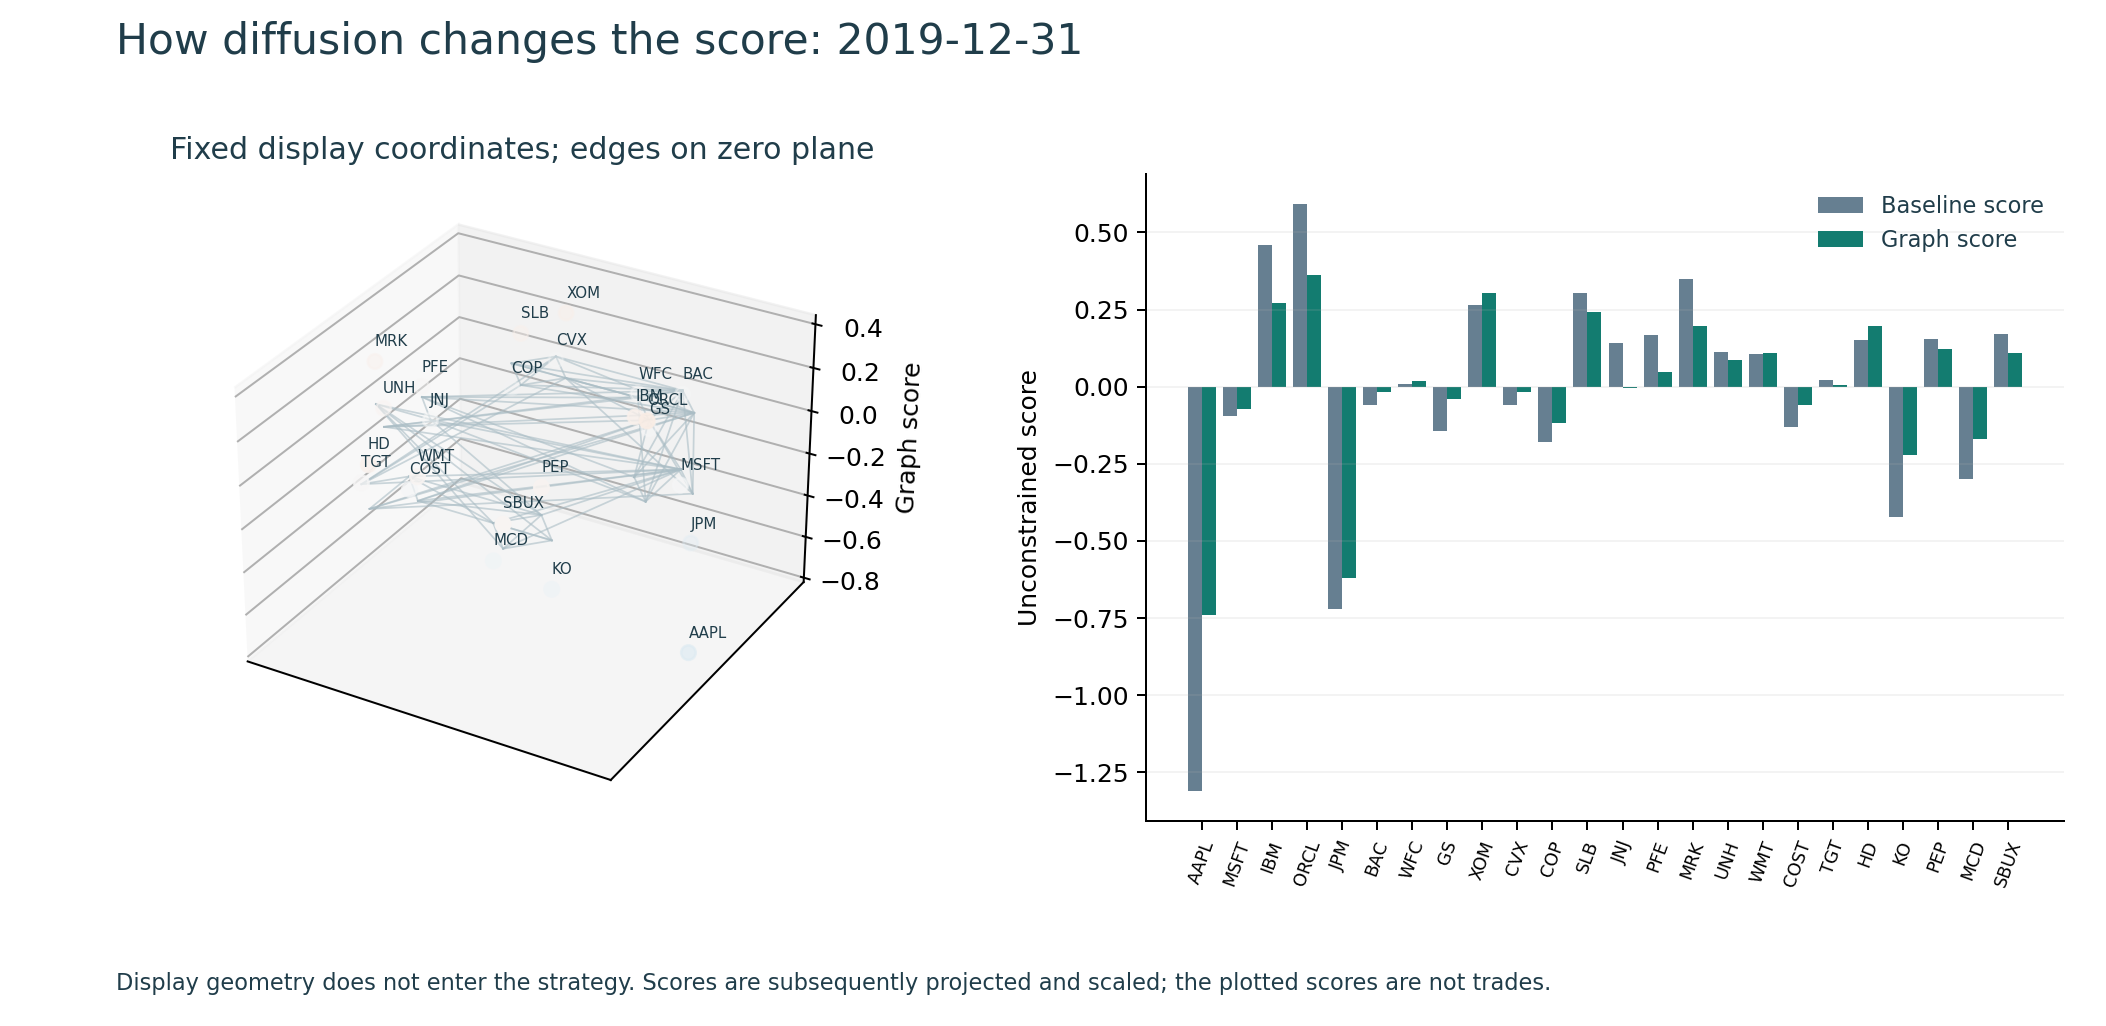
\includegraphics[width=\linewidth,height=.65\textheight,keepaspectratio]{assets/figure-08.png}

\caption{A historical graph and the resulting unconstrained scores}\label{fig:8}

\end{figure}

The companion \textbf{Graph-Diffusion-Explorer.html} shows 120 monthly graph snapshots, with a rotatable 3D network, date slider and paired score bars. Horizontal node coordinates are a fixed arrangement of the six research groups for display. Lines on the zero plane show retained connections; height shows the graph score. Neither drawing coordinates nor rendered interpolation enter the trading algorithm.


A positive plotted graph score proposes a long direction before the constraints are applied. The final projected weight may have a different sign. This distinction helps connect the mathematical operator to the implementation without presenting raw scores as actual trades or interpreting an attractive network visual as evidence of financial value.


\bodyheading{Persistent homology and simpler controls}

As Edelsbrunner et al. (2002) explain in \textit{Topological Persistence and Simplification}, a filtration records structure across scales through the birth and death of homological features. Here H0 describes component mergers and H1 describes cycles before they become boundaries of filled triangles. A triangle in the correlation network does not, by itself, constitute a persistent H1 feature. These objects describe the geometry of the observations; a financial interpretation requires a separate empirical argument.


Gidea and Katz (2018), in \textit{Topological data analysis of financial time series: Landscapes of crashes}, examine sliding-window point clouds of market-index returns. Their construction motivates asking whether topological summaries can describe financial structure. The present project instead treats the 24 assets as the points and constructs their distances from trailing return correlations. Consequently, this is not a replication of their experiment, and their findings cannot be transferred as evidence that this strategy forecasts crashes or earns positive returns.


\Needspace{4\baselineskip}\subsection{Frozen feature design and causal geometry}

\begingroup
\setcounter{table}{13}
\setstretch{1}\fontsize{10}{12.5}\selectfont
\renewcommand{\arraystretch}{1.12}
\arrayrulecolor{tablerule}
\begin{table}[!htbp]
\centering
\setstretch{1}\fontsize{10}{12.5}\selectfont
\begin{tabular}{P{0.300000\dimexpr\textwidth-4\tabcolsep\relax}P{0.700000\dimexpr\textwidth-4\tabcolsep\relax}}
\toprule
\rowcolor{tablehead} \textbf{Design choice} & \textbf{Declared implementation} \\ \midrule
Points & The same 24 assets; SPY is a volatility control, not a point \\
\midrule[0.2pt]
Observations & Trailing daily simple adjusted-price returns through close t \\
\midrule[0.2pt]
Windows & 126 sessions primary; 63 and 252 sessions retained as sensitivities \\
\midrule[0.2pt]
Geometry & Complete correlation distances, including negatively correlated pairs \\
\midrule[0.2pt]
Filtration & Vietoris–Rips; edge threshold \(\varepsilon\); coefficients in F\(_2\); H0 and H1 \\
\midrule[0.2pt]
Features & Mean and maximum finite H0 persistence; total and maximum finite H1 persistence \\
\midrule[0.2pt]
Controls & Same-window mean correlation, mean annualised stock volatility and annualised SPY volatility \\
\midrule[0.2pt]
Fitting & Descriptive OLS coefficients and control standardisation fitted on development only \\
\midrule[0.2pt]
Comparison dates & 2,516 common dates: 1,762 development and 754 validation \\
\midrule[0.2pt]
Trading interpretation & No return target, threshold fitting, strategy overlay or new backtest \\
\midrule[0.2pt]
Holdout at Milestone 4 & 2020–2025 was unavailable; release and final evaluation appear in Section 10 \\
\bottomrule
\end{tabular}
\caption{Topology protocol recorded before the first historical feature extraction}\label{tab:14}
\end{table}
\endgroup

The local record is {\fontsize{9.3}{12}\selectfont\nolinkurl{protocol/topology-features-v1.json}}, with SHA-256 {\fontsize{9.3}{12}\selectfont\nolinkurl{2b2d975392129a88ea10b5955dd9405be46d49ba2860f7d0e9872b0e76c926d1}}. It was locked before topology extraction, after the baseline and graph outcomes were already known. It is not external preregistration. No primary feature or window is selected after comparing the results.


As Mantegna (1999) explains in \textit{Hierarchical structure in financial markets}, return correlations can be transformed into distances for studying relationships between assets. \hyperref[eq:21]{Equation 21} uses that transformation. For the complete common observation window, it also follows directly from the Euclidean distance between centred, unit-length return vectors.


\paperequation{21}{Correlation distance as a Euclidean chord}{\begin{aligned}
 u_{i,t}&=\frac{r_{i,t-W_{\mathrm{len}}+1:t}-\bar r_{i,t}\mathbf{1}}{\left\|r_{i,t-W_{\mathrm{len}}+1:t}-\bar r_{i,t}\mathbf{1}\right\|_2},\\[4pt]
 d_{ij,t}&=\sqrt{2(1-\rho_{ij,t})}=\|u_{i,t}-u_{j,t}\|_2
 \end{aligned}}

Where: W\_len is the number of return observations and the mean is taken over that window. Constant series are rejected because the normalisation is undefined. Missing-data handling remains the exact-calendar rejection rule. The distance lies between zero and two; identical standardised histories can give zero distance between labelled assets. Neither thresholding the positive trading graph nor discarding negative correlations is part of this geometry.


\sourcemeta{Source: {\fontsize{9.3}{12}\selectfont\nolinkurl{market_neutral/topology.py}}, {\fontsize{9.3}{12}\selectfont\nolinkurl{correlation_distance}}; selected executable lines.}

\par\addvspace{4pt}\noindent\begin{minipage}{\linewidth}

\begin{Verbatim}[fontsize=\small,baselinestretch=1.0,breaklines=true,breakanywhere=true,breakautoindent=true,breakindent=10pt,frame=single,framerule=.3pt,rulecolor=\color{tablerule},framesep=6pt,numbersep=5pt,numbers=left,xleftmargin=15pt,formatcom=\color{black}]
centered = r - r.mean(axis=0)
norms = np.linalg.norm(centered, axis=0)
if (norms <= 1e-12).any():
    raise ValueError("Constant asset: correlation geometry is undefined")
unit = centered / norms
corr = np.clip(unit.T @ unit, -1., 1.)
corr = (corr + corr.T) / 2
np.fill_diagonal(corr, 1.)
distance = np.sqrt(2 * (1 - corr))
np.fill_diagonal(distance, 0.)
return corr, distance
\end{Verbatim}

\listingcaption{9}{Constructing the complete causal correlation geometry}

\end{minipage}\par\addvspace{4pt}

Features dated t include the return ending at t. They are available at that close and cannot earn an earlier return. Any future trading overlay would have to preserve the existing t+1 execution and t+2 first new-position return. A future-perturbation check replaces all later observations and confirms that earlier features are unchanged.


\Needspace{4\baselineskip}\subsection{Filtration, intervals and explicit boundary handling}

As Bauer (2021) describes in \textit{Ripser: efficient computation of Vietoris–Rips persistence barcodes}, efficient persistence calculations can operate on Rips filtrations. Tralie et al. (2018), in \textit{Ripser.py: A lean persistent homology library for Python}, provide the Python interface used here. The implementation fixes Ripser.py 0.6.14, homology coefficients modulo two and the full filtration through dimension one.


\paperequation{22}{Edge-threshold Vietoris–Rips complex}{\mathrm{VR}_{\varepsilon}(D_t)=\{\sigma\subseteq\{1,\ldots,n\}:\max_{i,j\in\sigma}d_{ij,t}\leq\varepsilon\}}

\hyperref[eq:22]{Equation 22} includes a simplex whenever all its pairwise distances are at most \(\varepsilon\). In particular, a three-vertex clique includes its filled triangle. The scale is an edge distance; replacing it with a ball-radius convention would change the numerical scale and is not done here.


In a full filtration on this finite cloud, one H0 interval persists indefinitely and all H1 intervals eventually die. The implementation excludes that one essential H0 interval from finite summaries and verifies that no essential H1 interval remains. It does not substitute an arbitrary finite value for infinity. Ripser omits zero-length intervals, so omitted zero-distance H0 mergers are restored as zero intervals when needed to retain the n\( - \)1 finite merger convention. This duplicate-point case is covered by a separate check; it does not occur in the historical extraction.


\paperequation{23}{Four predeclared persistence summaries}{\begin{aligned}
 \ell_a&=d_a-b_a,\\[3pt]
 f_{0,\mathrm{mean}}&=\frac{1}{n-1}\sum_{a\in\mathcal D_0^{\mathrm{fin}}}\ell_a,
 &f_{0,\max}&=\max_{a\in\mathcal D_0^{\mathrm{fin}}}\ell_a,\\[3pt]
 f_{1,\mathrm{total}}&=\sum_{a\in\mathcal D_1}\ell_a,
 &f_{1,\max}&=\max_{a\in\mathcal D_1}\ell_a
 \end{aligned}}

Where: b\_a and d\_a are birth and death thresholds, and \(\ell\)\_a is their difference. Empty H1 diagrams have total and maximum equal to zero. Every positive lifetime emitted by the engine is retained; there is no fitted significance or persistence cut-off. The features have distance units. The H0 merger distances agree with minimum spanning tree edge weights: both connect previously separate components in increasing distance order. The implementation is independently checked against SciPy's spanning-tree calculation on a known finite cloud.


\sourcemeta{Source: {\fontsize{9.3}{12}\selectfont\nolinkurl{market_neutral/topology.py}}, {\fontsize{9.3}{12}\selectfont\nolinkurl{persistence}}; selected executable lines. The complete function also validates the input and restores zero-distance H0 mergers.}

\par\addvspace{4pt}\noindent\begin{minipage}{\linewidth}

\begin{Verbatim}[fontsize=\small,baselinestretch=1.0,breaklines=true,breakanywhere=true,breakautoindent=true,breakindent=10pt,frame=single,framerule=.3pt,rulecolor=\color{tablerule},framesep=6pt,numbersep=5pt,numbers=left,xleftmargin=15pt,formatcom=\color{black}]
diagrams = ripser(d, distance_matrix=True, maxdim=1, coeff=2, thresh=np.inf)["dgms"]
h0, h1 = diagrams
essential = np.isinf(h0[:, 1])
if essential.sum() != 1 or not np.isfinite(h1).all():
    raise ValueError("Full finite Rips filtration must have one essential H0 and no essential H1")
h0 = h0[~essential].astype(float)
\end{Verbatim}

\listingcaption{10}{Full persistence calculation and essential-interval checks}

\end{minipage}\par\addvspace{4pt}

\Needspace{4\baselineskip}\subsection{Simpler controls and an honest redundancy check}

The controls are the mean of the off-diagonal correlations, the mean sample standard deviation of stock returns multiplied by \(\sqrt{252}\), and the sample standard deviation of SPY returns multiplied by \(\sqrt{252}\). Each uses the same window as the corresponding topological feature. Their purpose is to test whether an elaborate descriptor mostly reproduces a simpler observable.


Within-phase Spearman correlations compare rankings. The separate OLS calculation approximates each feature with the three controls. As Golub and Van Loan (2013) explain in \textit{Matrix Computations}, least-squares problems can be solved without explicitly inverting the normal-equations matrix; the implementation uses a least-squares solver and rejects a deficient design rank. The choice of these three controls is a project diagnostic, not a specification derived from that book.


\paperequation{24}{Development-only standardisation and control approximation}{\begin{aligned}
 z_{j,t}&=\frac{c_{j,t}-\bar c_{j,\mathrm{dev}}}{s_{j,\mathrm{dev}}},\\[3pt]
 \widehat\theta&=\arg\min_{\theta}\sum_{t\in\mathrm{dev}}\big(f_t-[1,z_t^\top]\theta\big)^2,\\[3pt]
 \widehat f_t&=[1,z_t^\top]\widehat\theta
 \end{aligned}}

Where: c\_j is a control, s\_j is its sample standard deviation and f is one of the four descriptors. Validation never enters centring, scaling or coefficient fitting. The outputs include coefficients and dated predictions/residuals for every window and feature. There are twelve fitted descriptive models, not twelve trading strategies.


\sourcemeta{Source: {\fontsize{9.3}{12}\selectfont\nolinkurl{market_neutral/topology.py}}, {\fontsize{9.3}{12}\selectfont\nolinkurl{fit_control_model}}; selected executable lines. The caller passes development observations only.}

\par\addvspace{4pt}\noindent\begin{minipage}{\linewidth}

\begin{Verbatim}[fontsize=\small,baselinestretch=1.0,breaklines=true,breakanywhere=true,breakautoindent=true,breakindent=10pt,frame=single,framerule=.3pt,rulecolor=\color{tablerule},framesep=6pt,numbersep=5pt,numbers=left,xleftmargin=15pt,formatcom=\color{black}]
x = train[list(CONTROLS)].to_numpy()
center, scale = x.mean(axis=0), x.std(axis=0, ddof=1)
if (scale <= 1e-12).any():
    raise ValueError("Constant development control")
design = np.column_stack([np.ones(len(x)), (x - center) / scale])
coefficients, _, rank, _ = np.linalg.lstsq(design, train[feature].to_numpy(), rcond=None)
\end{Verbatim}

\listingcaption{11}{Fitting controls only on the development segment}

\end{minipage}\par\addvspace{4pt}

\paperequation{25}{Phase-specific descriptive approximation score}{R^2_{\mathcal P}=1-\frac{\sum_{t\in\mathcal P}(f_t-\widehat f_t)^2}{\sum_{t\in\mathcal P}(f_t-\bar f_{\mathcal P})^2}}

The phase mean in \hyperref[eq:25]{Equation 25} is used only to score the approximation, not to fit it. Negative validation R\(^{2}\) is retained: it means that the transferred model has larger squared error than the constant validation-mean benchmark. A low R\(^{2}\) does not establish novelty, predictability or a trading benefit; it can also reflect a limited functional form, estimation noise or distribution change. Overlapping windows induce dependence, so no independent-observation p-values are attached to these diagnostics.


\begingroup
\setcounter{table}{14}
\setstretch{1}\fontsize{10}{12.5}\selectfont
\renewcommand{\arraystretch}{1.12}
\arrayrulecolor{tablerule}
\begin{table}[!htbp]
\centering
\setstretch{1}\fontsize{10}{12.5}\selectfont
\begin{tabular}{P{0.440000\dimexpr\textwidth-6\tabcolsep\relax}Q{0.280000\dimexpr\textwidth-6\tabcolsep\relax}Q{0.280000\dimexpr\textwidth-6\tabcolsep\relax}}
\toprule
\rowcolor{tablehead} \textbf{Feature} & \textbf{Development} & \textbf{Validation} \\ \midrule
H0 mean & -0.935 & -0.968 \\
\midrule[0.2pt]
H0 maximum & -0.879 & -0.890 \\
\midrule[0.2pt]
H1 total & -0.593 & -0.667 \\
\midrule[0.2pt]
H1 maximum & -0.463 & -0.421 \\
\bottomrule
\end{tabular}
\caption{Primary-window Spearman correlation with mean correlation}\label{tab:15}
\end{table}
\endgroup

\begingroup
\setcounter{table}{15}
\setstretch{1}\fontsize{10}{12.5}\selectfont
\renewcommand{\arraystretch}{1.12}
\arrayrulecolor{tablerule}
\begin{table}[!htbp]
\centering
\setstretch{1}\fontsize{10}{12.5}\selectfont
\begin{tabular}{P{0.440000\dimexpr\textwidth-6\tabcolsep\relax}Q{0.280000\dimexpr\textwidth-6\tabcolsep\relax}Q{0.280000\dimexpr\textwidth-6\tabcolsep\relax}}
\toprule
\rowcolor{tablehead} \textbf{Feature} & \textbf{Development} & \textbf{Validation} \\ \midrule
H0 mean & 0.959 & 0.563 \\
\midrule[0.2pt]
H0 maximum & 0.810 & -0.195 \\
\midrule[0.2pt]
H1 total & 0.345 & 0.343 \\
\midrule[0.2pt]
H1 maximum & 0.223 & 0.303 \\
\bottomrule
\end{tabular}
\caption{Primary-window feature approximation using development-fitted controls; R\(^{2}\)}\label{tab:16}
\end{table}
\endgroup

\begingroup
\setcounter{table}{16}
\setstretch{1}\fontsize{10}{12.5}\selectfont
\renewcommand{\arraystretch}{1.12}
\arrayrulecolor{tablerule}
\begin{table}[!htbp]
\centering
\setstretch{1}\fontsize{10}{12.5}\selectfont
\begin{tabular}{P{0.220000\dimexpr\textwidth-10\tabcolsep\relax}Q{0.195000\dimexpr\textwidth-10\tabcolsep\relax}Q{0.195000\dimexpr\textwidth-10\tabcolsep\relax}Q{0.195000\dimexpr\textwidth-10\tabcolsep\relax}Q{0.195000\dimexpr\textwidth-10\tabcolsep\relax}}
\toprule
\rowcolor{tablehead} \textbf{Feature} & \textbf{Development: 63} & \textbf{Development: 252} & \textbf{Validation: 63} & \textbf{Validation: 252} \\ \midrule
H0 mean & 0.785 & 0.723 & 0.713 & 0.764 \\
\midrule[0.2pt]
H0 maximum & 0.792 & 0.700 & 0.652 & 0.630 \\
\midrule[0.2pt]
H1 total & 0.396 & 0.285 & 0.535 & 0.477 \\
\midrule[0.2pt]
H1 maximum & 0.249 & 0.082 & 0.293 & 0.297 \\
\bottomrule
\end{tabular}
\caption{Paired-date Spearman correlations with the primary 126-session feature}\label{tab:17}
\end{table}
\endgroup

\begin{figure}[!htbp]

\centering

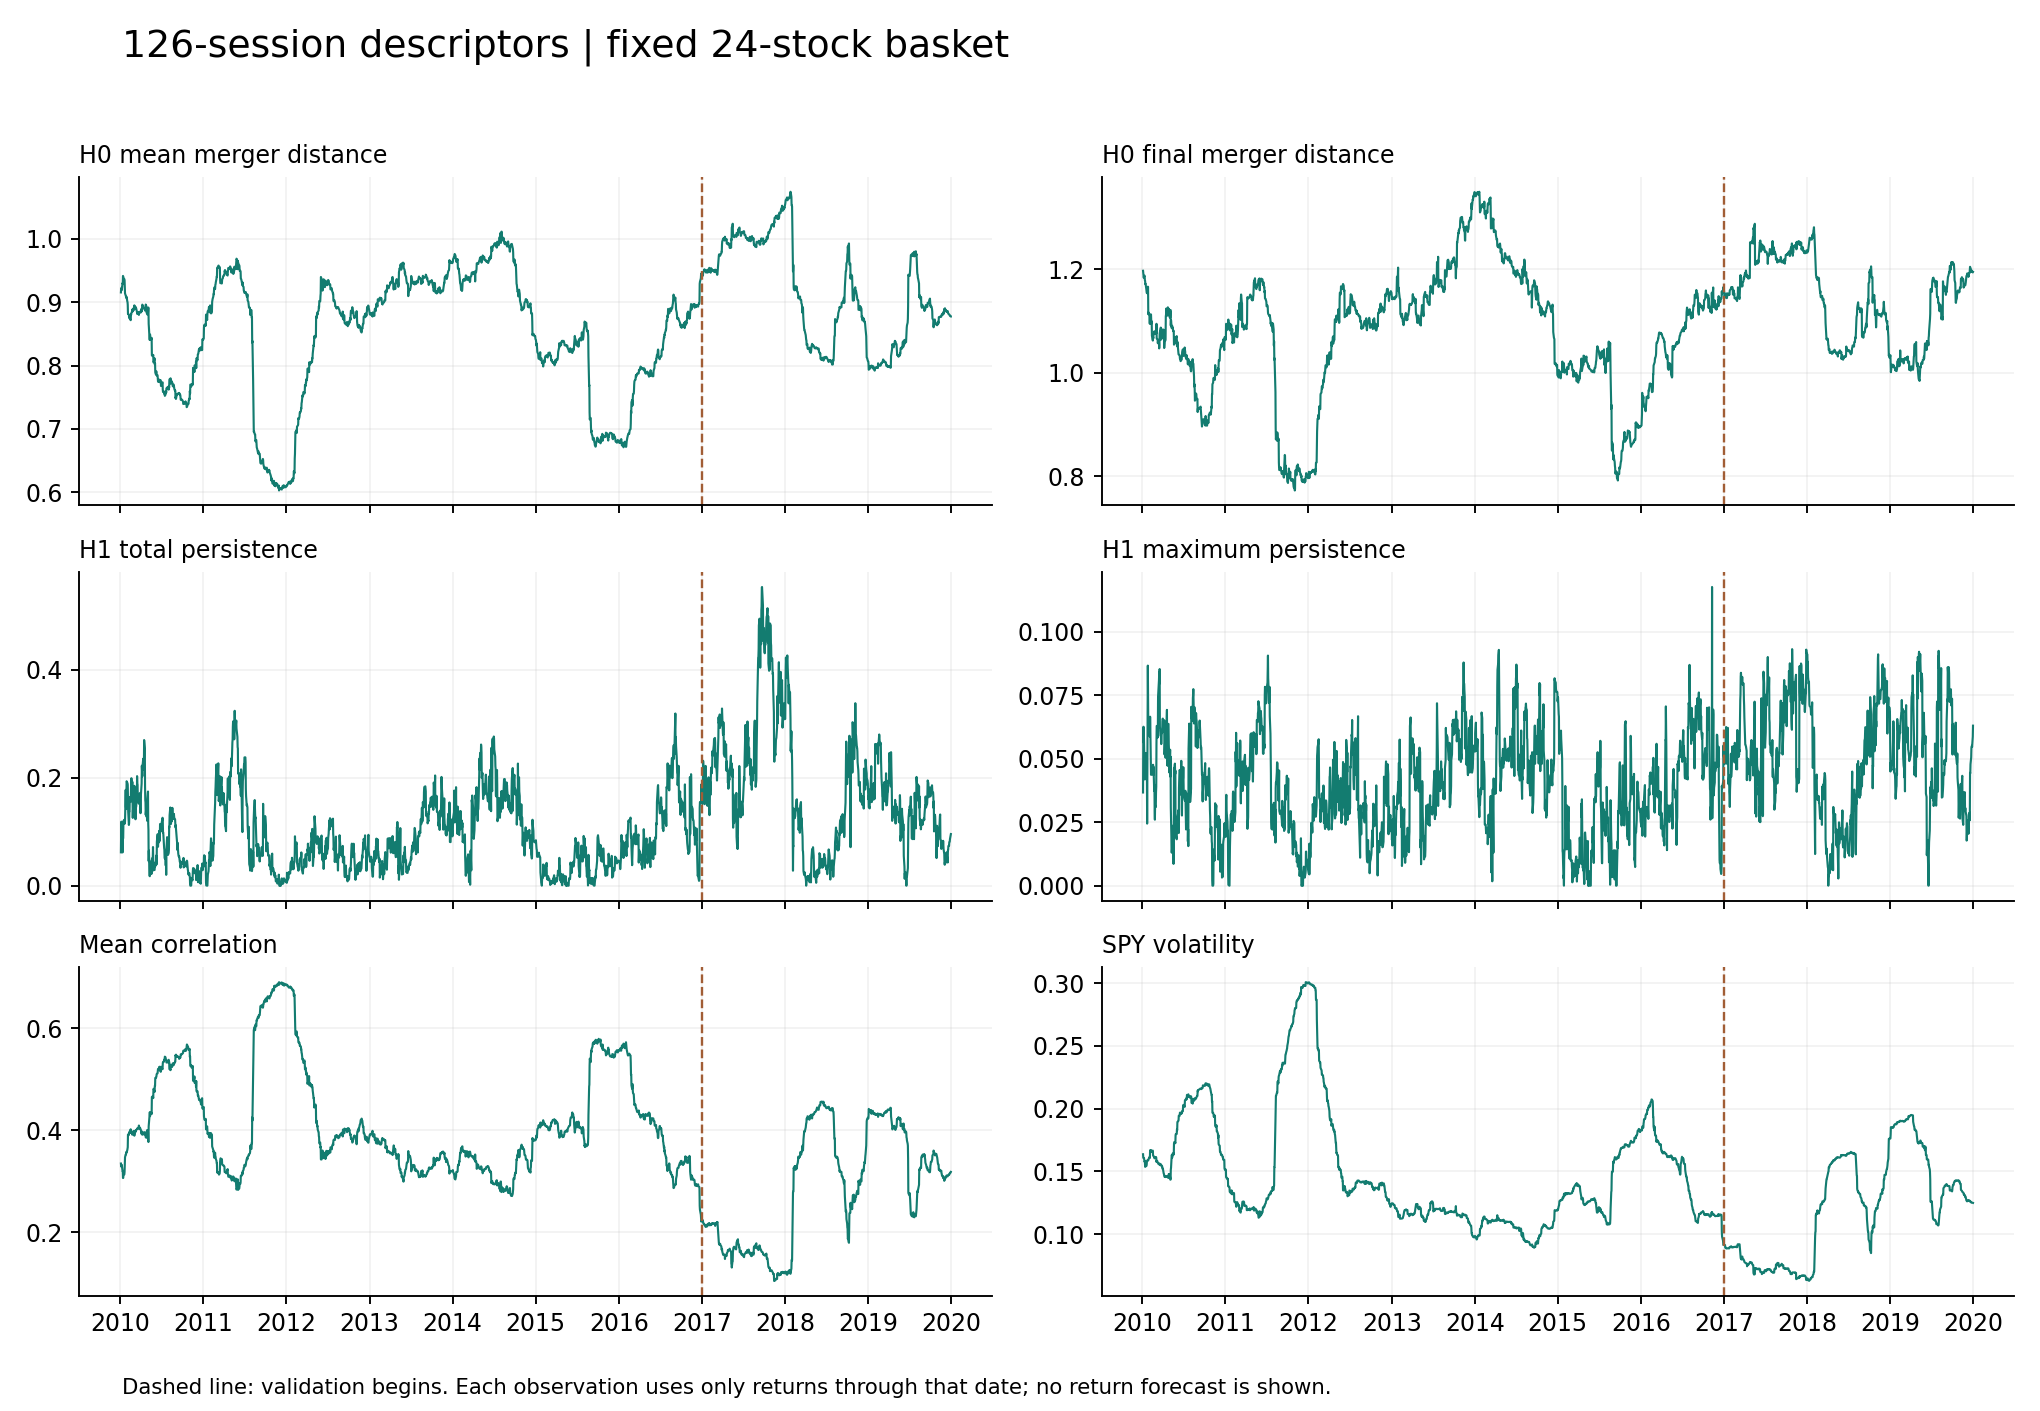
\includegraphics[width=\linewidth,height=.65\textheight,keepaspectratio]{assets/figure-09.png}

\caption{Primary-window topology descriptors and simpler market measures}\label{fig:9}

\end{figure}

\begin{figure}[!htbp]

\centering

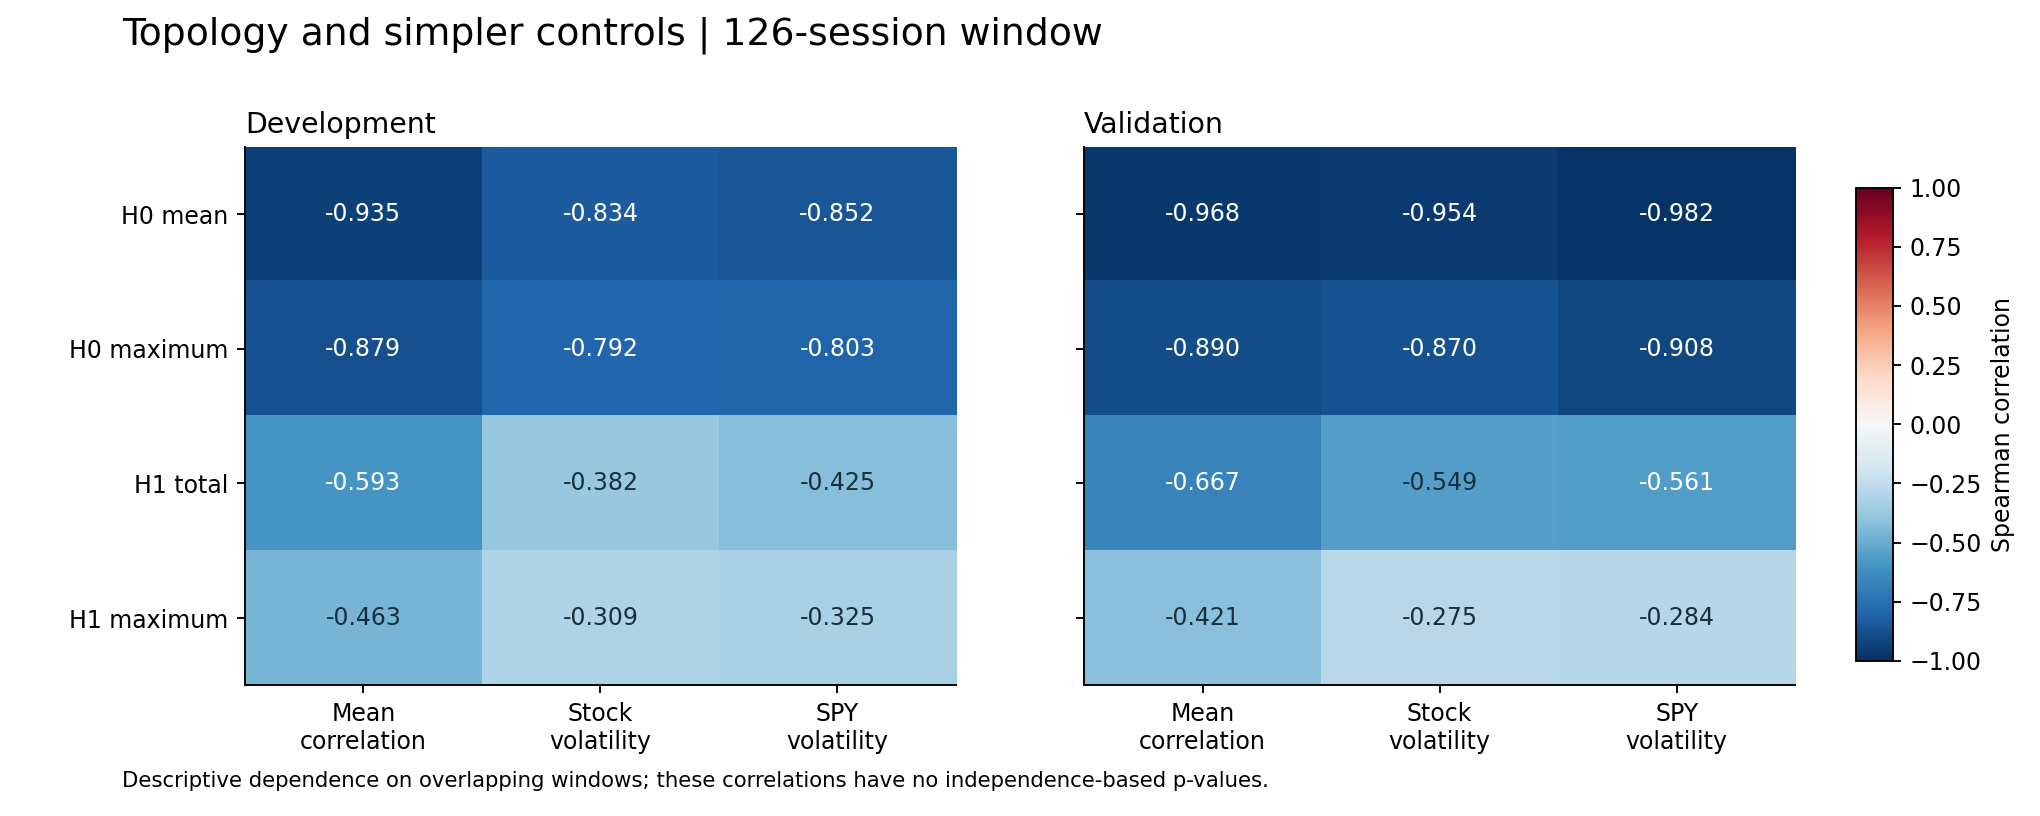
\includegraphics[width=\linewidth,height=.65\textheight,keepaspectratio]{assets/figure-10.png}

\caption{Spearman dependence between topology features and simple controls}\label{fig:10}

\end{figure}

H0 mean persistence largely follows the ordinary correlation level. The OLS approximation for H0 maximum fits development reasonably well but transfers poorly, with validation R\(^{2}\) below zero. This is a concrete setback for treating the same fitted relation as stable across phases. It is preserved in the record; the validation segment is not used to re-estimate the model and produce a more attractive score.


H1 retains variation not captured by the declared linear control model. That observation is insufficient to promote it into a trading signal. In particular, the window comparison below shows that the identity and duration of cycles change considerably with the estimation horizon. None of the three windows is selected as a winner after this analysis.


\Needspace{4\baselineskip}\subsection{Window sensitivity and diagram stability}

As Chazal et al. (2014) explain in \textit{Persistence stability for geometric complexes}, Rips persistence diagrams can be controlled by changes in the underlying metric geometry. For the same labelled assets, matching each asset to itself gives the specialisation in \hyperref[eq:26]{Equation 26}. This is a bound on diagram changes, not a statement that every summary or financial relationship stays constant when the return window changes.


\paperequation{26}{Same-label perturbation bound for Rips diagrams}{d_B\big(\mathcal D_q(D),\mathcal D_q(D')\big)\leq\eta,\qquad\eta=\max_{i,j}|D_{ij}-D'_{ij}|,\quad q\in\{0,1\}}

Where: d\_B is bottleneck distance, allowing intervals to match to the diagonal. The matching essential H0 intervals are omitted on both sides of the finite computation. The full finite complexes use the same edge-threshold convention. The numerical comparison permits 2\(\times\)10\(^{-6}\) for the engine's finite precision; it does not relax the theoretical bound for a statistical reason.


All 480 declared checks satisfy the bound: 120 month-end dates, two alternative windows and two homology dimensions. The checks use real distances for each window and compare them with the primary 126-session matrix. They validate numerical consistency with the bound. Empirical feature stability is assessed separately by paired-date rank correlations.


\begin{figure}[!htbp]

\centering

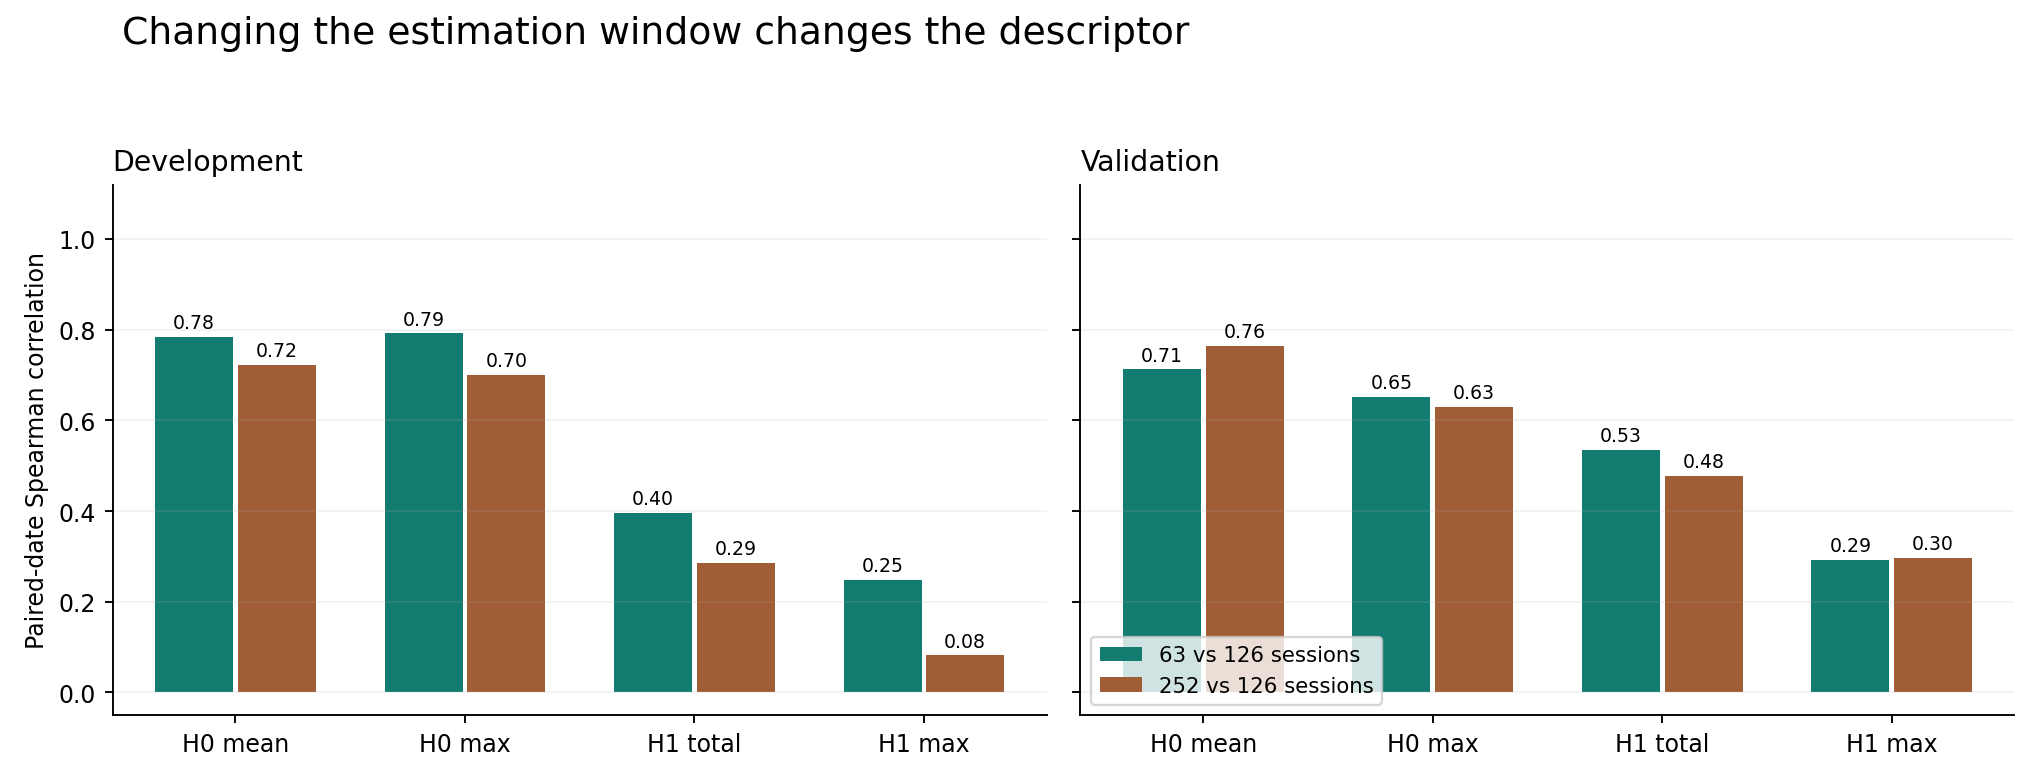
\includegraphics[width=\linewidth,height=.65\textheight,keepaspectratio]{assets/figure-11.png}

\caption{Feature sensitivity to the declared estimation windows}\label{fig:11}

\end{figure}

H1 maximum persistence is particularly sensitive: its development rank correlation between 252 and 126 sessions is approximately 0.082. Passing the diagram bound therefore cannot be advertised as robust regime classification. Before a future overlay could be considered, a new protocol would need to state which feature and horizon it intends to use, why the decision is justified, and how dependence and model selection will be handled.


\Needspace{4\baselineskip}\subsection{Dynamic three-dimensional explanation}

As Bubenik (2015) explains in \textit{Statistical topological data analysis using persistence landscapes}, intervals can be mapped to ordered tent functions. \hyperref[eq:27]{Equation 27} defines the landscape used in the interactive companion. The complete interval set supplies the numerical descriptors; the display shows only its first five ranks on a fixed grid from zero to two.


\paperequation{27}{Persistence landscape from ordered interval tents}{\begin{aligned}
 g_a(\varepsilon)&=\max\{0,\min(\varepsilon-b_a,d_a-\varepsilon)\},\\[3pt]
 \lambda_k(\varepsilon)&=\operatorname{kth\ largest}_{a}\,g_a(\varepsilon)
 \end{aligned}}

Where: k is a positive integer and unavailable ranks have value zero. Each height has distance units. The interpolation joining integer ranks in the 3D surface is a display choice; it does not define additional topological observations and is not a fitted financial surface.


\sourcemeta{Source: {\fontsize{9.3}{12}\selectfont\nolinkurl{market_neutral/topology.py}}, {\fontsize{9.3}{12}\selectfont\nolinkurl{landscape}}; selected executable lines.}

\par\addvspace{4pt}\noindent\begin{minipage}{\linewidth}

\begin{Verbatim}[fontsize=\small,baselinestretch=1.0,breaklines=true,breakanywhere=true,breakautoindent=true,breakindent=10pt,frame=single,framerule=.3pt,rulecolor=\color{tablerule},framesep=6pt,numbersep=5pt,numbers=left,xleftmargin=15pt,formatcom=\color{black}]
x = np.asarray(grid, dtype=float)
tents = np.maximum(0, np.minimum(x[None, :] - bars[:, :1], bars[:, 1:] - x[None, :]))
ordered = np.sort(tents, axis=0)[::-1]
out = np.zeros((layers, len(x)))
out[:min(layers, len(bars))] = ordered[:layers]
return out
\end{Verbatim}

\listingcaption{12}{Computing ordered landscape layers from the actual intervals}

\end{minipage}\par\addvspace{4pt}

\begin{figure}[!htbp]

\centering

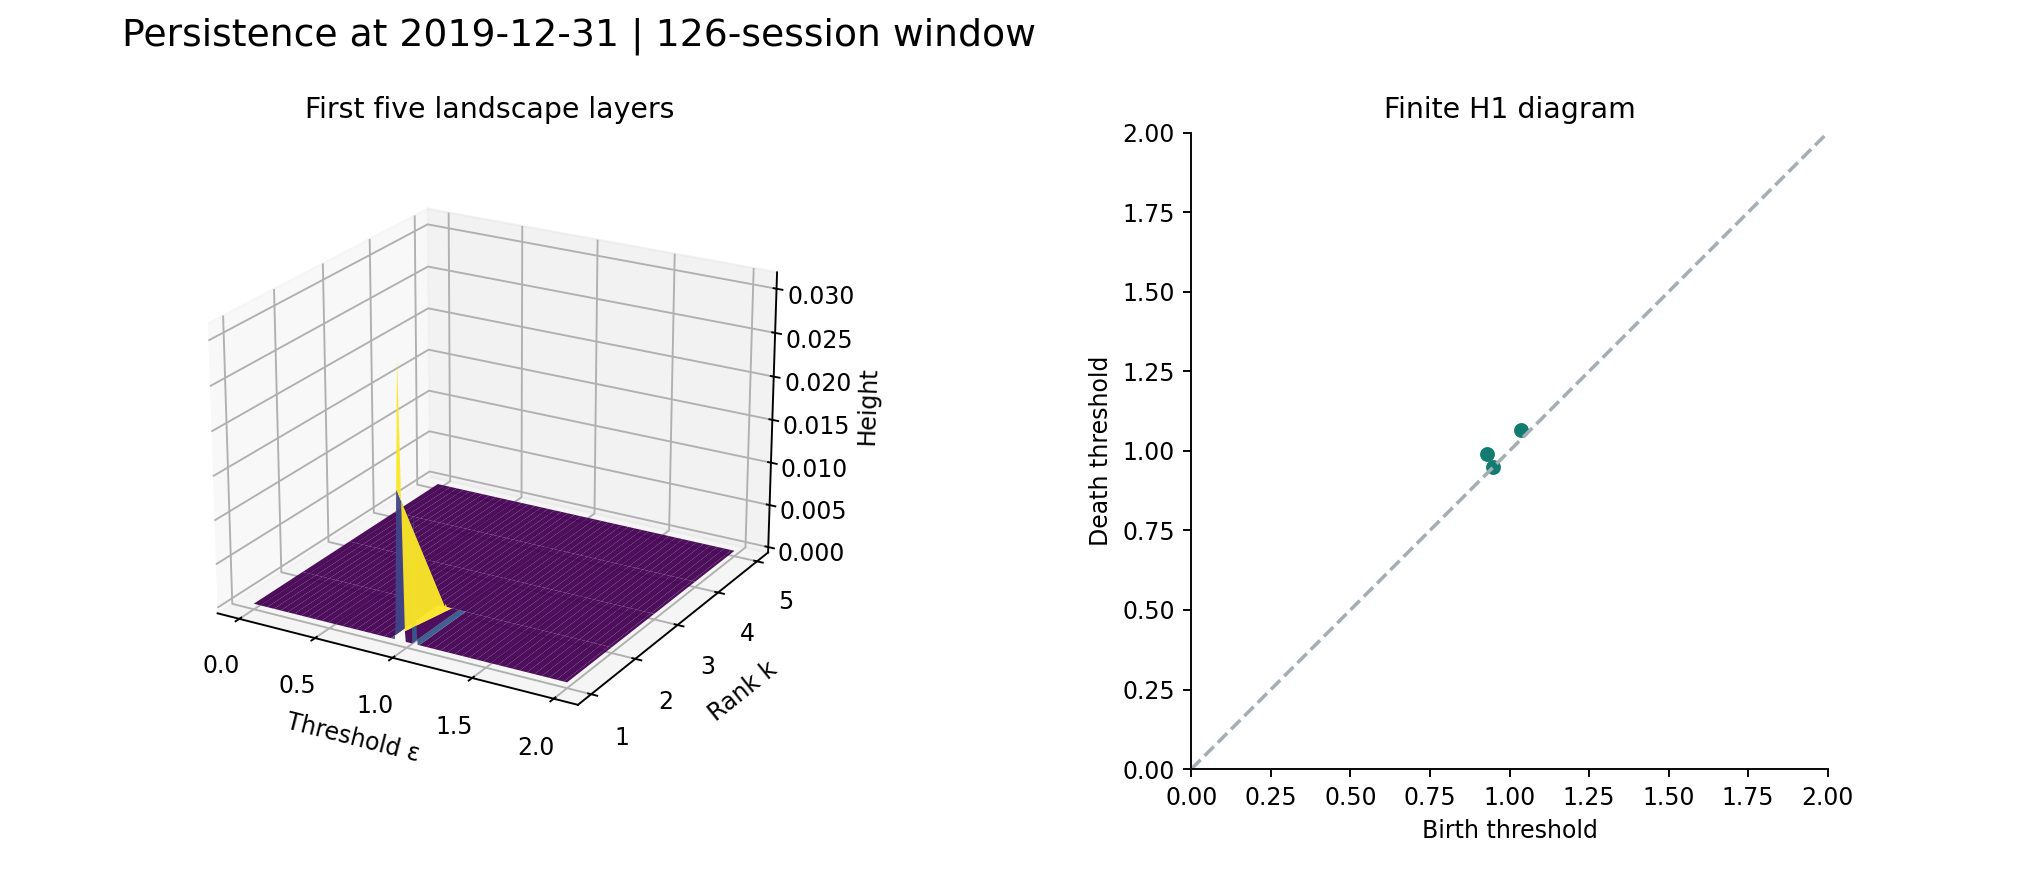
\includegraphics[width=.86\linewidth,height=.65\textheight,keepaspectratio]{assets/figure-12.png}

\caption{H1 landscape and birth–death diagram at the last validation month-end}\label{fig:12}

\end{figure}

{\fontsize{9.3}{12}\selectfont\nolinkurl{outputs/topology/Persistence-Landscape-Explorer.html}} contains 120 primary-window monthly frames, rotatable 3D layers, a paired birth–death diagram, date selection and playback. Axes remain fixed through playback and JavaScript is embedded for offline use. Structural checks verify frame counts, matching dates, layer values and control configuration. Live browser interaction is not claimed as tested in the build environment.


Ten new focused automated checks cover the square, triangle and line examples; an independent spanning-tree comparison; duplicate points; correlation-distance invariance; future-data isolation; analytic landscape tents; a perturbed-metric bound; control fitting; and invalid geometry. At the completion of this stage, 35 tests passed; the final evaluation expands the suite to 41. The extraction produces 7,548 dated window rows in approximately three seconds in the recorded environment; this timing excludes plots and diagram-distance checks and is not a hardware-independent performance claim.


\bodyheading{Final evaluation on the reserved 2020–2025 period}

The final experiment evaluates the fixed primary graph strategy against the original baseline. It does not introduce a topology trading overlay. That decision was made before acquisition: the completed descriptor study showed substantial overlap with simple correlation for H0 and material window sensitivity for H1, without establishing a defensible trading direction or threshold. Retaining the simpler trading comparison is a research decision recorded in the final protocol, not a claim that topology can never be useful.


As White (2000) explains in \textit{A Reality Check for Data Snooping}, searching across alternatives changes the interpretation of apparent success. Bailey et al. (2017), in \textit{The probability of backtest overfitting}, also discuss the risk associated with repeated selection. The final protocol therefore fixes the comparison, finite scenario set, uncertainty procedure and evidence conditions before the reserved observations are acquired. Neither cited procedure is implemented as a retrospective correction for every decision made in this project.


\Needspace{4\baselineskip}\subsection{Release, data audit and interpretation of “reserved”}

The final protocol is {\fontsize{9.3}{12}\selectfont\nolinkurl{protocol/final-evaluation-v1.json}}, SHA-256 {\fontsize{9.3}{12}\selectfont\nolinkurl{8fdee505de9ceaa8e4a2951deba29c1305eb12ee64d2d42467a978e2805c2acd}}. Its lock precedes acquisition. The previous three protocols and the original observations are preserved, and the existing strategy, graph, portfolio, accounting, inference and topology calculation files are checked against their frozen source hashes.


\begingroup
\setcounter{table}{17}
\setstretch{1}\fontsize{10}{12.5}\selectfont
\renewcommand{\arraystretch}{1.12}
\arrayrulecolor{tablerule}
\begin{table}[!htbp]
\centering
\setstretch{1}\fontsize{10}{12.5}\selectfont
\begin{tabular}{P{0.320000\dimexpr\textwidth-4\tabcolsep\relax}P{0.680000\dimexpr\textwidth-4\tabcolsep\relax}}
\toprule
\rowcolor{tablehead} \textbf{Item} & \textbf{Frozen decision} \\ \midrule
Primary comparison & Graph, \(\tau\) = 1, against the baseline on 2020–2025 \\
\midrule[0.2pt]
Data and warm-up & Separate coherent adjusted-price vintage; 2019 returns with a 31 December 2018 anchor \\
\midrule[0.2pt]
Universe & Same 24 stocks and SPY; no stock/date substitution \\
\midrule[0.2pt]
Primary costs & 5 bps per dollar traded and 2\% annual short borrow \\
\midrule[0.2pt]
Finite scenario set & 16 model/fee cases, four additional borrow cases and two matched-gross cases \\
\midrule[0.2pt]
Primary uncertainty & 10,000 paired stationary-bootstrap replicates; mean block length 10 \\
\midrule[0.2pt]
Inference family & Baseline mean, graph mean and graph-minus-baseline mean; Bonferroni adjustment for these three \\
\midrule[0.2pt]
Secondary checks & Block lengths 5/20, HAC with ten lags, matched-gross paired intervals and every calendar year \\
\midrule[0.2pt]
Necessary condition 1 & Primary graph CAGR is positive at default costs \\
\midrule[0.2pt]
Necessary condition 2 & Adjusted lower bound for the graph's arithmetic mean is positive \\
\midrule[0.2pt]
Necessary condition 3 & Adjusted lower bound for the graph-minus-baseline mean is positive \\
\midrule[0.2pt]
Necessary condition 4 & Matched-gross paired 95\% lower bound is positive \\
\midrule[0.2pt]
Topology & Descriptors and development-fitted control relationships only; no new overlay \\
\bottomrule
\end{tabular}
\caption{Final design and evidence conditions fixed before acquisition}\label{tab:18}
\end{table}
\endgroup

The new Yahoo Finance (2026b) responses contain 1,761 aligned price observations per series from 31 December 2018 through 31 December 2025. There are 1,508 evaluation sessions, from 2 January 2020 to 31 December 2025. Every series exactly matches the observed SPY calendar; missing values, nonpositive reported volumes and adjusted-return moves above the predeclared 40\% audit threshold are absent. The earlier Yahoo Finance (2026a) cache remains unchanged.


Adjusted-price levels can differ across retrievals. Comparing levels alone could mistake a constant adjustment factor for a meaningful return revision. \hyperref[eq:28]{Equation 28} instead checks the common 2019 return history before evaluation. The new calculation uses its own complete warm-up and test vintage; it does not splice a price from the old cache into a new adjusted series.


\paperequation{28}{Overlapping-return vintage audit}{\max_{t\in\mathcal O}\left|\left(\frac{P^{\mathrm{new}}_t}{P^{\mathrm{new}}_{t-1}}-1\right)-\left(\frac{P^{\mathrm{old}}_t}{P^{\mathrm{old}}_{t-1}}-1\right)\right|\leq 10^{-5}}

Where: O is the 252-return overlap in 2019. The tolerance is 0.1 basis points per daily return and was fixed before the download. The observed maximum across the 25 series is approximately 1.154\(\times\)10\(^{-6}\), or 0.0115 basis points, within that tolerance. The final processed snapshot hash is {\fontsize{9.3}{12}\selectfont\nolinkurl{040f3199669d24009b848b5d1112321a70b7cb8084cb84fce6d6878a33abdcdd}}. A retained snapshot guard prevents a later acquisition from silently becoming the same experiment. Its timestamp records the audited vintage for replay and is distinct from the earlier protocol lock.


\sourcemeta{Source: {\fontsize{9.3}{12}\selectfont\nolinkurl{market_neutral/final_data.py}}, {\fontsize{9.3}{12}\selectfont\nolinkurl{overlap_audit}}; selected executable lines. The complete function rejects mismatched dates and deviations above the frozen tolerance.}

\par\addvspace{4pt}\noindent\begin{minipage}{\linewidth}

\begin{Verbatim}[fontsize=\small,baselinestretch=1.0,breaklines=true,breakanywhere=true,breakautoindent=true,breakindent=10pt,frame=single,framerule=.3pt,rulecolor=\color{tablerule},framesep=6pt,numbersep=5pt,numbers=left,xleftmargin=15pt,formatcom=\color{black}]
old = original.pct_change(fill_method=None).iloc[1:]
new = latest.pct_change(fill_method=None).iloc[1:]
difference = (new - old).abs()
maximum = float(difference.max())
ratios = latest / original
\end{Verbatim}

\listingcaption{13}{Auditing return changes rather than adjusted-price level changes}

\end{minipage}\par\addvspace{4pt}

“Reserved” describes the order of work inside this project. These are publicly known historical years, and the basket was selected retrospectively from surviving companies. As Shumway (1997) explains in \textit{The Delisting Bias in CRSP Data}, omitted adverse outcomes can matter for historical inference. This project's broader survivor-selection limitation affects the final period too. A pre-acquisition hash does not transform the study into a prospective blind experiment or repair the absence of a point-in-time universe.


\Needspace{4\baselineskip}\subsection{Primary performance and the accounting explanation}

\begingroup
\setcounter{table}{18}
\setstretch{1}\fontsize{10}{12.5}\selectfont
\renewcommand{\arraystretch}{1.12}
\arrayrulecolor{tablerule}
\begin{table}[!htbp]
\centering
\setstretch{1}\fontsize{10}{12.5}\selectfont
\begin{tabular}{P{0.460000\dimexpr\textwidth-6\tabcolsep\relax}Q{0.270000\dimexpr\textwidth-6\tabcolsep\relax}Q{0.270000\dimexpr\textwidth-6\tabcolsep\relax}}
\toprule
\rowcolor{tablehead} \textbf{Measure} & \textbf{Baseline} & \textbf{Graph, \(\tau\) = 1} \\ \midrule
CAGR & -5.57\% & -4.80\% \\
\midrule[0.2pt]
Total return & -29.02\% & -25.52\% \\
\midrule[0.2pt]
Maximum drawdown & -31.69\% & -28.61\% \\
\midrule[0.2pt]
Annualised volatility & 5.97\% & 4.66\% \\
\midrule[0.2pt]
Mean gross exposure & 66.12\% & 63.48\% \\
\midrule[0.2pt]
Mean daily turnover & 41.69\% & 41.08\% \\
\midrule[0.2pt]
Realised full-period SPY beta & 0.0330 & 0.0315 \\
\bottomrule
\end{tabular}
\caption{Reserved-test primary outcomes at 5 bps and 2\% annual short borrow}\label{tab:19}
\end{table}
\endgroup

Both strategies lose money at the default costs. The graph loses less over the full period, but its \( - \)4.80\% CAGR is still negative. Its lower volatility and smaller drawdown are descriptive findings under the stated constraints and data; they do not establish a profitable or superior risk-adjusted policy. Estimated neutrality remains numerically satisfied, while realised market beta can differ from zero.


\begin{figure}[!htbp]

\centering

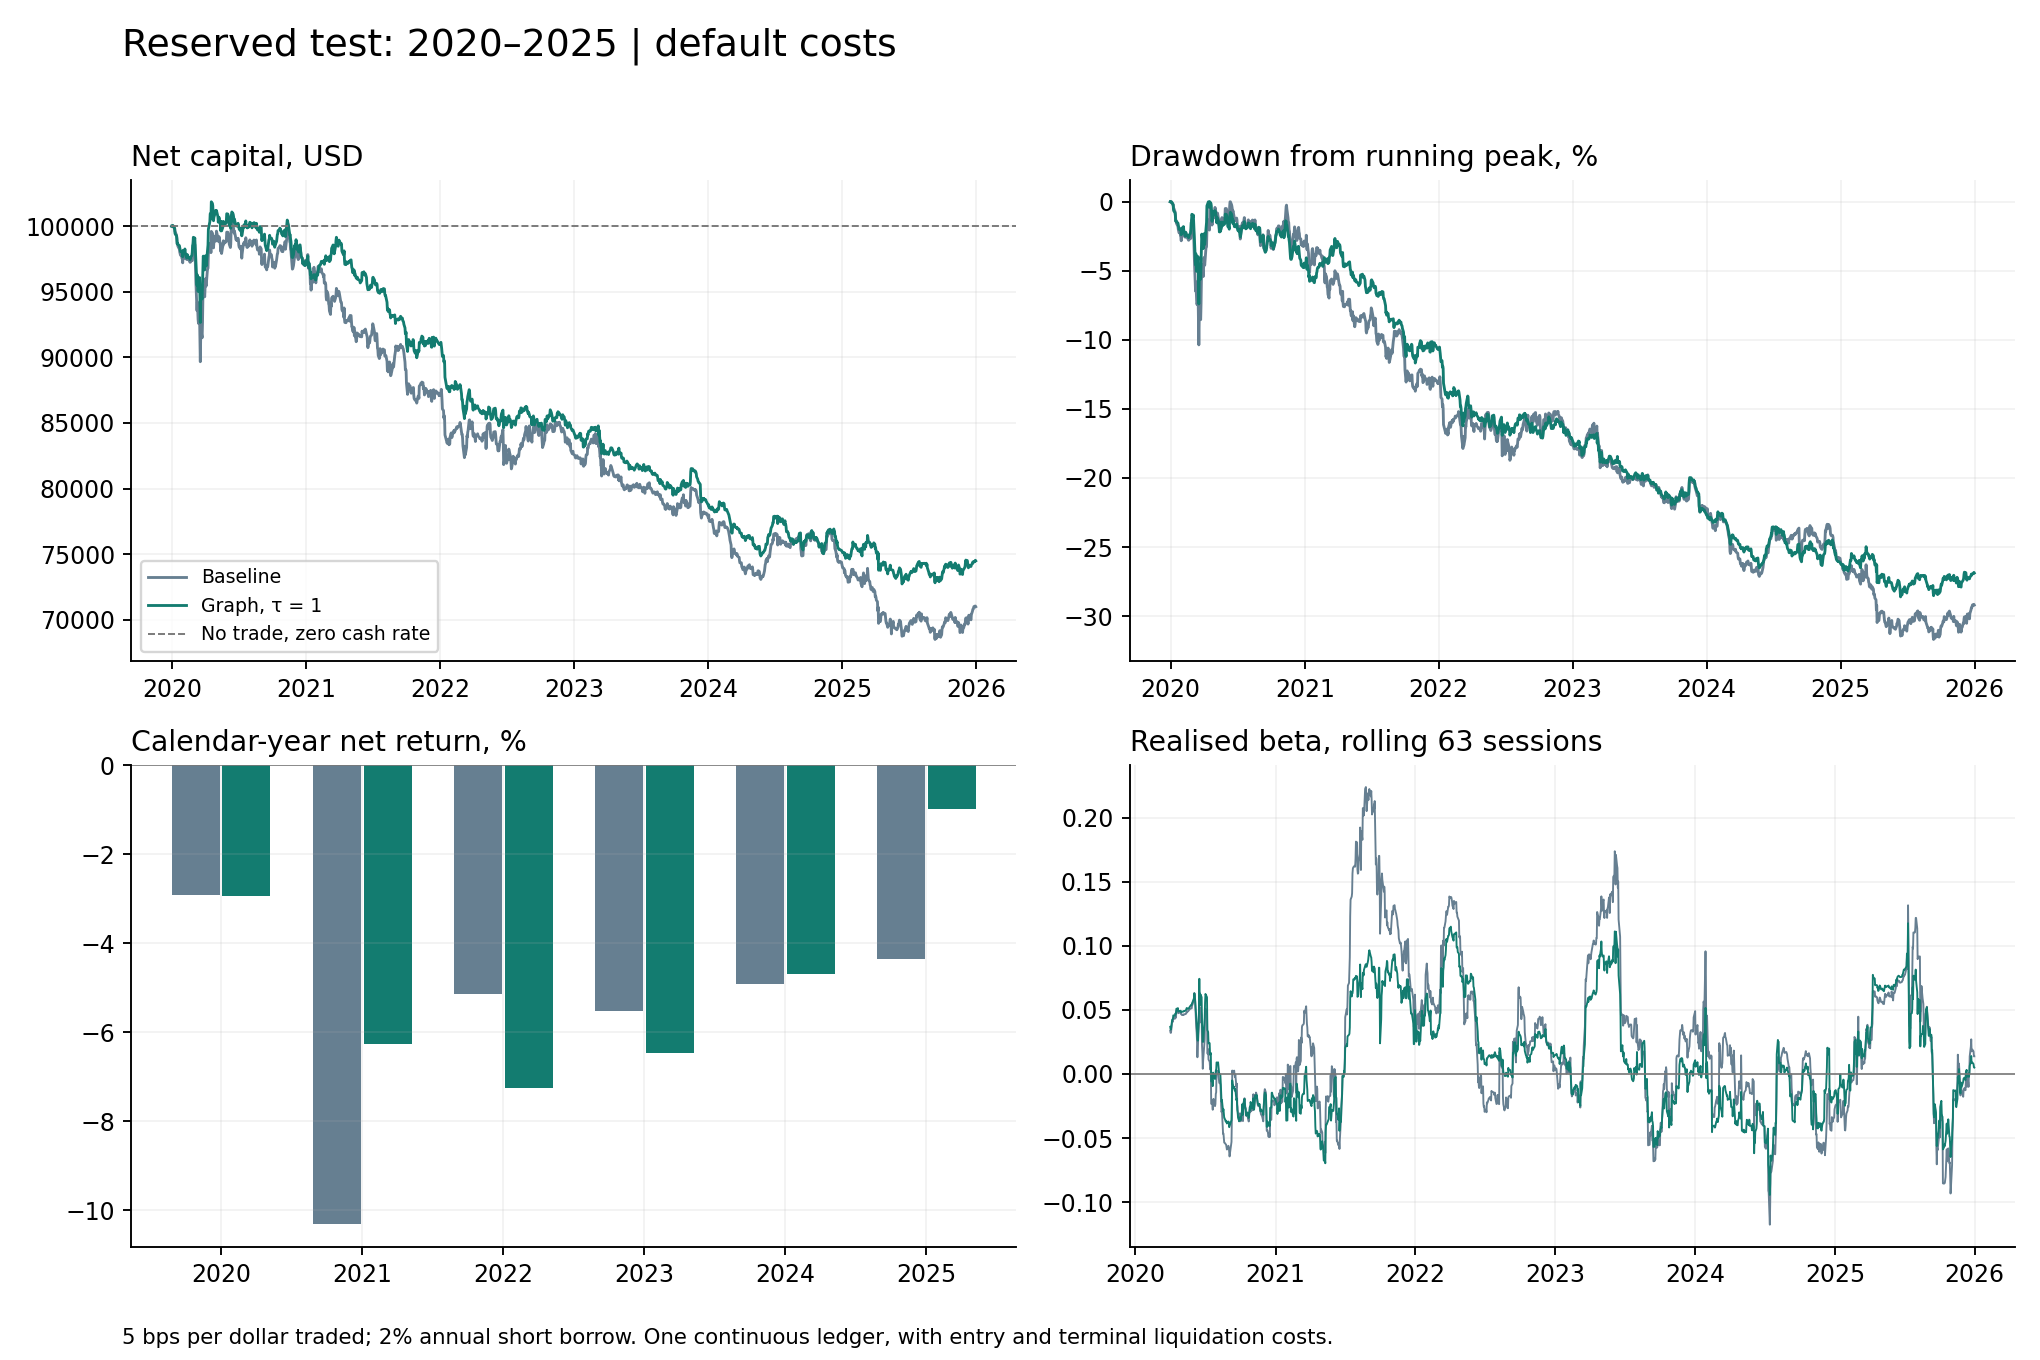
\includegraphics[width=\linewidth,height=.65\textheight,keepaspectratio]{assets/figure-13.png}

\caption{Final-test capital, drawdown, annual returns and realised beta}\label{fig:13}

\end{figure}

The zero-cash-rate no-trade line in \hyperref[fig:13]{Figure 13} is an accounting comparator consistent with the omitted cash-interest model. It is not a historical risk-free return series. The ledger starts flat with USD 100,000, uses the preceding close's decision for first execution, and includes entry fees and liquidation at the last test close. Calendar-year summaries do not reset the book or remove losses at year boundaries.


The primary graph's annualised arithmetic gross contribution is approximately +1.00\%, compared with 5.18\% trading drag and 0.64\% borrow drag, leaving \( - \)4.81\% net. The baseline has +0.37\% gross contribution, 5.25\% trading drag and 0.67\% borrow drag, leaving \( - \)5.55\% net. These components reconcile arithmetically under \hyperref[eq:12]{Equation 12}. Their scaling is different from CAGR, and summing them should not be represented as a compounded-return decomposition.


\Needspace{4\baselineskip}\subsection{Joint uncertainty for three explicit comparisons}

Politis and Romano (1994), in \textit{The Stationary Bootstrap}, provide the dependence-preserving resampling construction. Nordman (2009), in \textit{A note on the stationary bootstrap's variance}, provides the algorithmic and finite-variance relationship used by the earlier numerical checks. The final calculation applies one index matrix to the paired daily returns so that each bootstrap replicate preserves their contemporaneous relationship.


\paperequation{29}{Three predeclared daily comparisons}{\xi_t=\begin{pmatrix}R^{B,\mathrm{net}}_t\\R^{G,\mathrm{net}}_t\\R^{G,\mathrm{net}}_t-R^{B,\mathrm{net}}_t\end{pmatrix},
 \qquad \widehat\mu_j=252\,\overline{\xi}_j,\quad j=1,2,3}

The first two means compare with the zero-cash-rate no-trade reference; the third measures incremental arithmetic return. The stationary bootstrap uses 10,000 replicates, primary expected block length ten and fixed seeds. All declared block-length results and the Newey and West (1987) HAC cross-check are retained. No estimator is selected because it gives the preferred conclusion.


\sourcemeta{Source: {\fontsize{9.3}{12}\selectfont\nolinkurl{market_neutral/final_inference.py}}, {\fontsize{9.3}{12}\selectfont\nolinkurl{fixed_family_intervals}}; selected executable lines. The assertion checks the pairing identity within each replicate.}

\par\addvspace{4pt}\noindent\begin{minipage}{\linewidth}

\begin{Verbatim}[fontsize=\small,baselinestretch=1.0,breaklines=true,breakanywhere=true,breakautoindent=true,breakindent=10pt,frame=single,framerule=.3pt,rulecolor=\color{tablerule},framesep=6pt,numbersep=5pt,numbers=left,xleftmargin=15pt,formatcom=\color{black}]
indices = stationary_indices(len(paired),settings["stationary_bootstrap_replicates"],length,
                             settings["seed"]+length)
# Each column sees the same blocks; the difference is paired path by path.
means = np.column_stack([values[:,j][indices].mean(axis=1) for j in range(3)])
np.testing.assert_allclose(means[:,2],means[:,1]-means[:,0],atol=1e-15)
\end{Verbatim}

\listingcaption{14}{Applying identical resampling blocks to all paired comparisons}

\end{minipage}\par\addvspace{4pt}

As Lehmann and Romano (2005) explain in \textit{Testing Statistical Hypotheses}, Chapter 9, considering several hypotheses requires distinguishing an individual error probability from a family-wise error probability. The present family has three predeclared means. \hyperref[eq:30]{Equation 30} states the union-bound argument used to allocate the error budget; it does not require independence between the three comparisons.


\paperequation{30}{Bonferroni allocation for the fixed three-mean family}{\begin{gathered}
 \Pr\!\left(\bigcup_{j=1}^{m_F}\{\mu_j\notin I_j\}\right)
 \leq\sum_{j=1}^{m_F}\Pr(\mu_j\notin I_j)\leq\alpha,\\[4pt]
 m_F=3,\qquad\alpha=0.05,\\[4pt]
 \Pr(\mu_j\in I_j)\geq1-\frac{\alpha}{m_F}=0.98333\ldots
 \end{gathered}}

For the bootstrap, \hyperref[eq:30]{Equation 30} is an approximate-coverage design because each marginal interval is itself approximate. The percentile bounds use the 0.008333… and 0.991666… quantiles; the pointwise 95\% intervals are also shown. Bonferroni controls only the stated family conditional on adequate marginal coverage. It does not correct survivorship, structural changes, data revisions or an unlimited history of model searches. HAC intervals share the same reporting levels but rely on their own asymptotic approximation.


\begingroup
\setcounter{table}{19}
\setstretch{1}\fontsize{10}{12.5}\selectfont
\renewcommand{\arraystretch}{1.12}
\arrayrulecolor{tablerule}
\begin{table}[!htbp]
\centering
\setstretch{1}\fontsize{10}{12.5}\selectfont
\begin{tabular}{P{0.320000\dimexpr\textwidth-8\tabcolsep\relax}Q{0.140000\dimexpr\textwidth-8\tabcolsep\relax}Q{0.270000\dimexpr\textwidth-8\tabcolsep\relax}Q{0.270000\dimexpr\textwidth-8\tabcolsep\relax}}
\toprule
\rowcolor{tablehead} \textbf{Comparison} & \textbf{Estimate} & \textbf{Pointwise 95\% interval} & \textbf{Bonferroni 98.33\% interval} \\ \midrule
Baseline versus zero cash rate & -5.55 & [-10.21, -0.80] & [-11.24, +0.32] \\
\midrule[0.2pt]
Graph versus zero cash rate & -4.81 & [-8.44, -1.08] & [-9.32, -0.14] \\
\midrule[0.2pt]
Graph minus baseline & +0.73 & [-1.66, +3.25] & [-2.14, +3.85] \\
\bottomrule
\end{tabular}
\caption{Annualised arithmetic means and stationary-bootstrap intervals; percentage points}\label{tab:20}
\end{table}
\endgroup

\begin{figure}[!htbp]

\centering

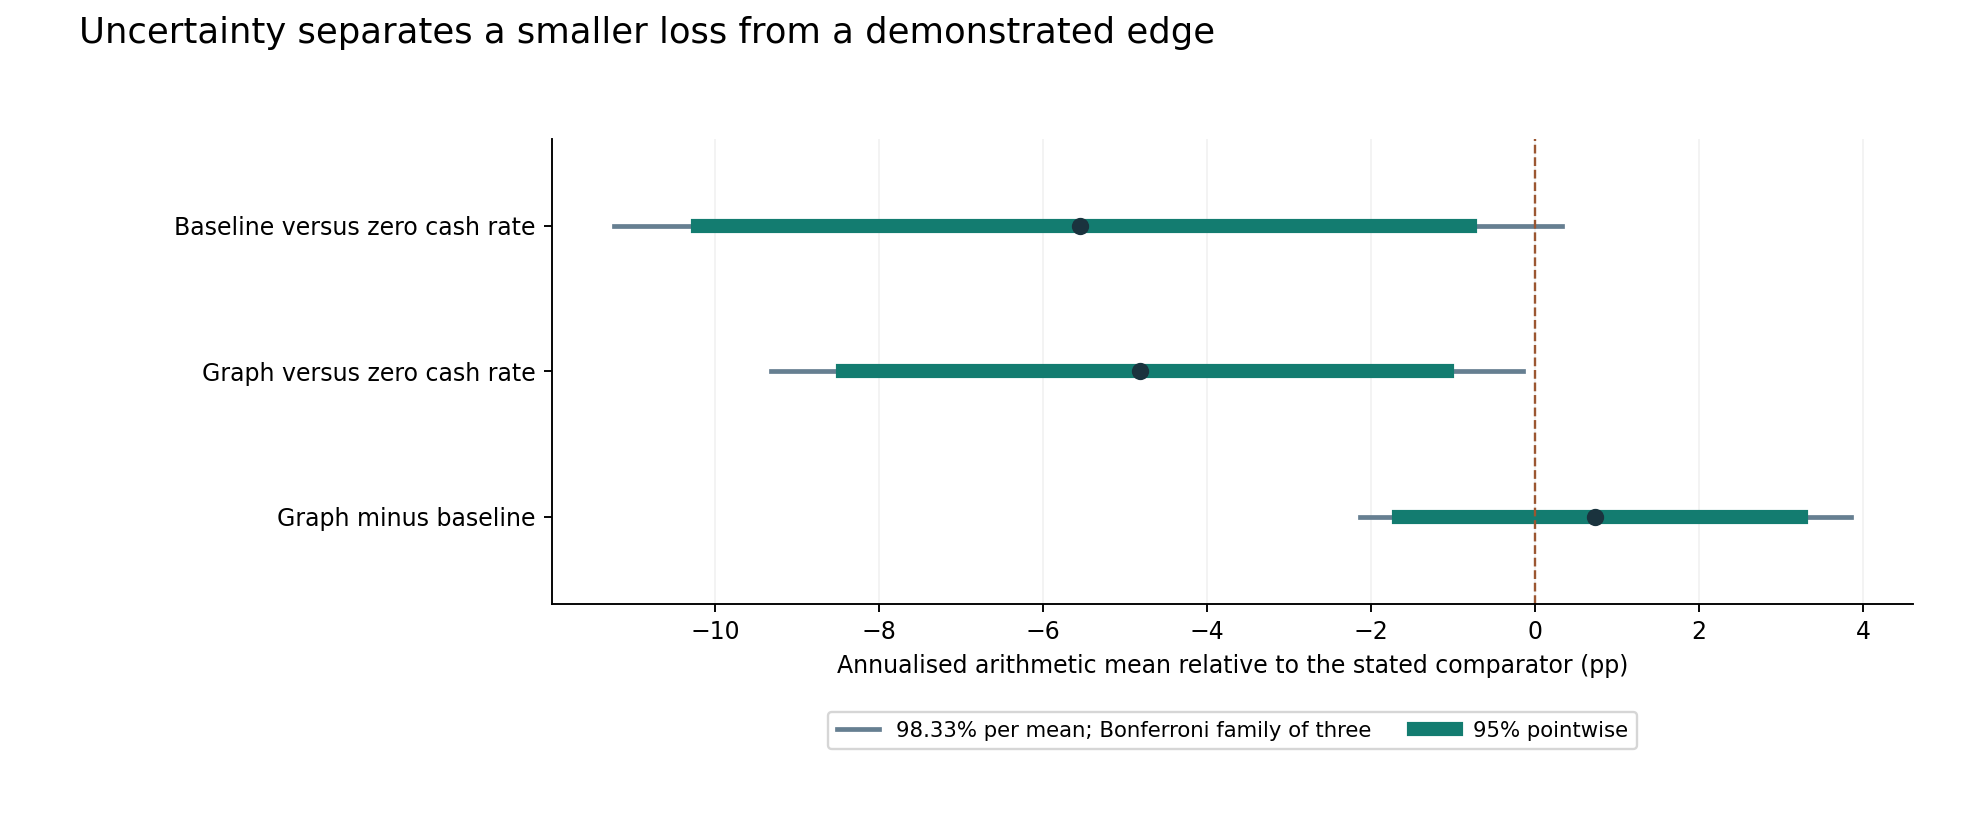
\includegraphics[width=\linewidth,height=.65\textheight,keepaspectratio]{assets/figure-14.png}

\caption{Pointwise and family-adjusted intervals for the final arithmetic comparisons}\label{fig:14}

\end{figure}

The graph-minus-baseline point estimate is +0.73 percentage points per year in arithmetic terms. Its adjusted interval spans \( - \)2.14 to +3.85 percentage points, so the sign of the incremental mean is unresolved by this procedure. It would be incorrect to replace this estimand with the +0.76-percentage-point CAGR difference or to describe either statistic as evidence of a positive absolute return.


The primary graph's adjusted mean interval remains below zero under the chosen bootstrap settings. The overall evidence decision nevertheless uses the four frozen necessary conditions in \hyperref[tab:18]{Table 18} rather than a favourable reinterpretation of individual intervals. None of those four conditions is met.


\Needspace{4\baselineskip}\subsection{Exposure and cost controls retain the negative finding}

\begingroup
\setcounter{table}{20}
\setstretch{1}\fontsize{10}{12.5}\selectfont
\renewcommand{\arraystretch}{1.12}
\arrayrulecolor{tablerule}
\begin{table}[!htbp]
\centering
\setstretch{1}\fontsize{10}{12.5}\selectfont
\begin{tabular}{P{0.460000\dimexpr\textwidth-6\tabcolsep\relax}Q{0.270000\dimexpr\textwidth-6\tabcolsep\relax}Q{0.270000\dimexpr\textwidth-6\tabcolsep\relax}}
\toprule
\rowcolor{tablehead} \textbf{Measure} & \textbf{Baseline matched} & \textbf{Graph matched} \\ \midrule
CAGR & -4.94\% & -4.69\% \\
\midrule[0.2pt]
Mean gross exposure & 59.57\% & 59.57\% \\
\midrule[0.2pt]
Mean daily turnover & 37.97\% & 38.60\% \\
\bottomrule
\end{tabular}
\caption{Matched-gross control at the default costs}\label{tab:21}
\end{table}
\endgroup

At matched gross, baseline and graph CAGR are approximately \( - \)4.94\% and \( - \)4.69\%. The arithmetic paired difference is +0.21 percentage points, with a pointwise 95\% stationary-bootstrap interval from \( - \)1.97 to +2.44. Equal gross does not equal equal risk, but this control again reduces the observed performance difference without establishing a reliable improvement.


\begingroup
\setcounter{table}{21}
\setstretch{1}\fontsize{10}{12.5}\selectfont
\renewcommand{\arraystretch}{1.12}
\arrayrulecolor{tablerule}
\begin{table}[!htbp]
\centering
\setstretch{1}\fontsize{10}{12.5}\selectfont
\begin{tabular}{P{0.280000\dimexpr\textwidth-10\tabcolsep\relax}Q{0.180000\dimexpr\textwidth-10\tabcolsep\relax}Q{0.180000\dimexpr\textwidth-10\tabcolsep\relax}Q{0.180000\dimexpr\textwidth-10\tabcolsep\relax}Q{0.180000\dimexpr\textwidth-10\tabcolsep\relax}}
\toprule
\rowcolor{tablehead} \textbf{Model} & \textbf{0 bps} & \textbf{5 bps} & \textbf{10 bps} & \textbf{20 bps} \\ \midrule
Baseline & -0.47\% & -5.57\% & -10.40\% & -19.34\% \\
\midrule[0.2pt]
Graph \(\tau\) = 0.5 & 0.39\% & -4.62\% & -9.38\% & -18.20\% \\
\midrule[0.2pt]
Graph \(\tau\) = 1 & 0.25\% & -4.80\% & -9.61\% & -18.50\% \\
\midrule[0.2pt]
Graph \(\tau\) = 2 & -0.06\% & -5.13\% & -9.94\% & -18.84\% \\
\bottomrule
\end{tabular}
\caption{Every declared fee/diffusion case: final-test CAGR; borrow fixed at 2\%}\label{tab:22}
\end{table}
\endgroup

\begingroup
\setcounter{table}{22}
\setstretch{1}\fontsize{10}{12.5}\selectfont
\renewcommand{\arraystretch}{1.12}
\arrayrulecolor{tablerule}
\begin{table}[!htbp]
\centering
\setstretch{1}\fontsize{10}{12.5}\selectfont
\begin{tabular}{P{0.280000\dimexpr\textwidth-6\tabcolsep\relax}Q{0.360000\dimexpr\textwidth-6\tabcolsep\relax}Q{0.360000\dimexpr\textwidth-6\tabcolsep\relax}}
\toprule
\rowcolor{tablehead} \textbf{Annual short borrow} & \textbf{Baseline} & \textbf{Graph, \(\tau\) = 1} \\ \midrule
0\% & -4.94\% & -4.19\% \\
\midrule[0.2pt]
2\% & -5.57\% & -4.80\% \\
\midrule[0.2pt]
5\% & -6.50\% & -5.71\% \\
\bottomrule
\end{tabular}
\caption{Every declared borrow case: final-test CAGR; trading cost fixed at 5 bps}\label{tab:23}
\end{table}
\endgroup

The zero-trading-fee primary graph case has a small positive CAGR of approximately +0.25\%, with borrow still charged. That scenario does not justify discarding the specified 5 bps fee: at default costs the same candidate loses 4.80\% annually. Nor is diffusion time 0.5 promoted because it looks slightly better. Every sensitivity case remains a reported check of the original primary design.


\begin{figure}[!htbp]

\centering

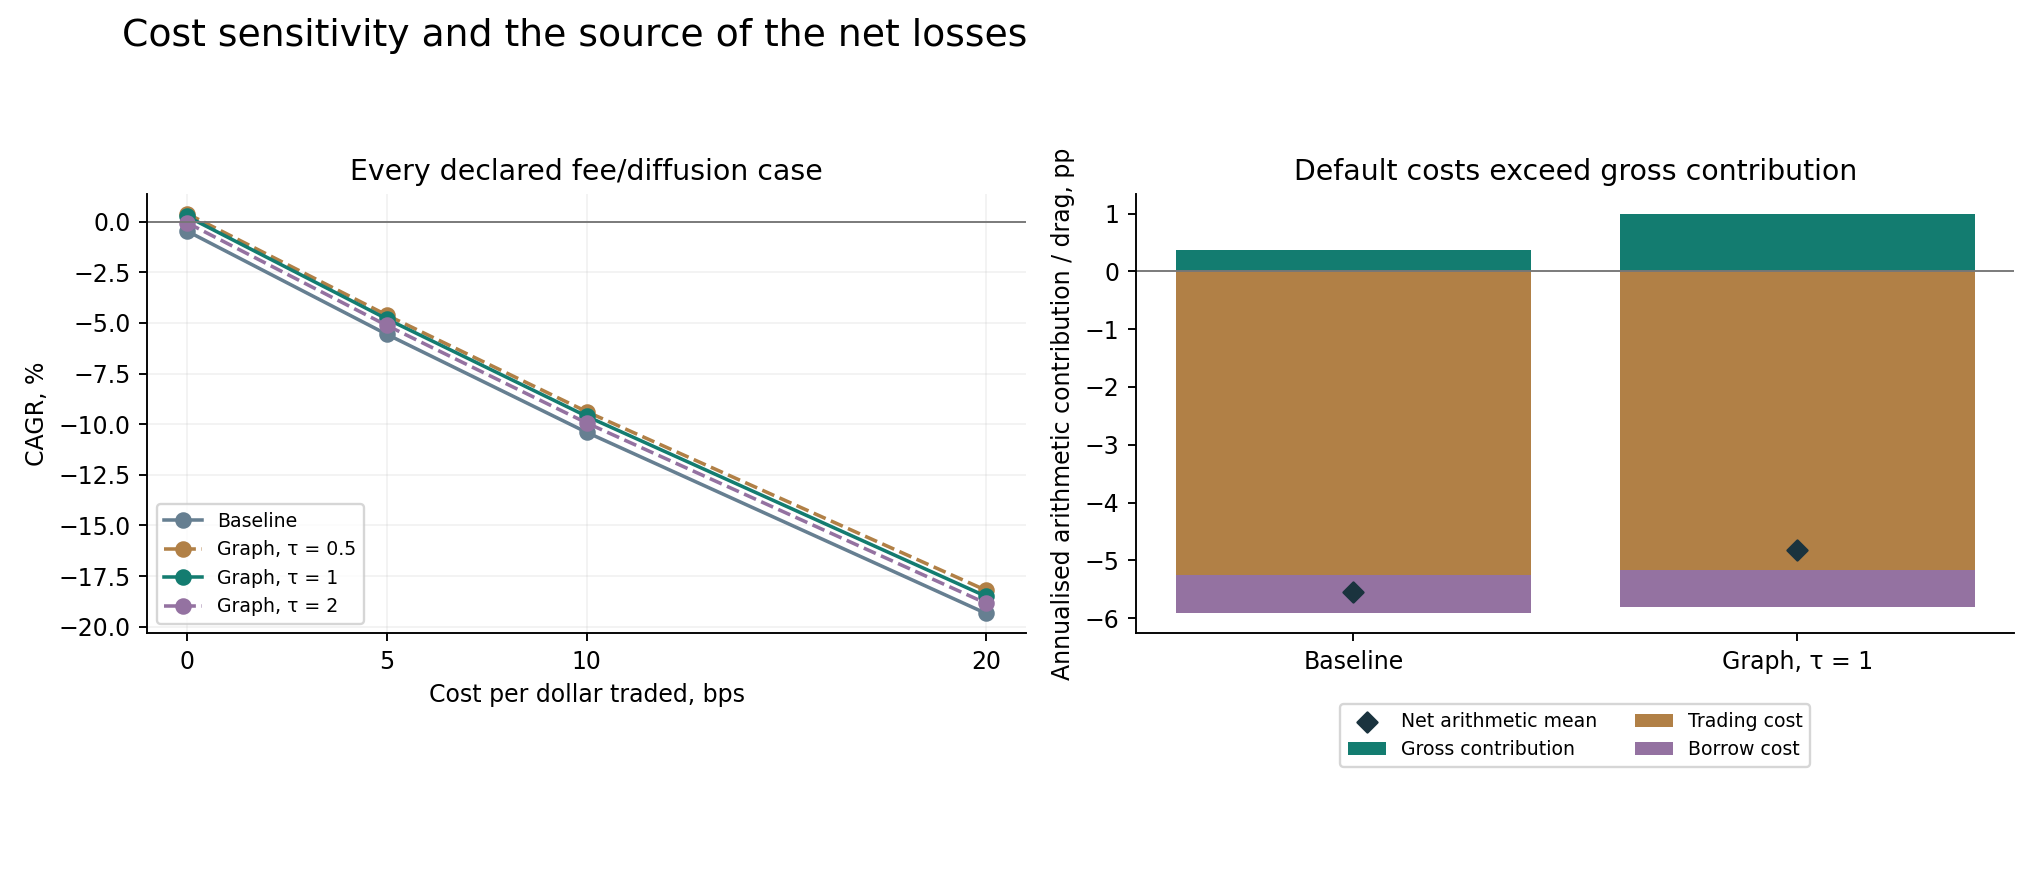
\includegraphics[width=\linewidth,height=.65\textheight,keepaspectratio]{assets/figure-15.png}

\caption{Final-test fee sensitivity and arithmetic cost decomposition}\label{fig:15}

\end{figure}

\begingroup
\setcounter{table}{23}
\setstretch{1}\fontsize{10}{12.5}\selectfont
\renewcommand{\arraystretch}{1.12}
\arrayrulecolor{tablerule}
\begin{table}[!htbp]
\centering
\setstretch{1}\fontsize{10}{12.5}\selectfont
\begin{tabular}{P{0.240000\dimexpr\textwidth-6\tabcolsep\relax}Q{0.380000\dimexpr\textwidth-6\tabcolsep\relax}Q{0.380000\dimexpr\textwidth-6\tabcolsep\relax}}
\toprule
\rowcolor{tablehead} \textbf{Year} & \textbf{Baseline} & \textbf{Graph, \(\tau\) = 1} \\ \midrule
2020 & -2.92\% & -2.93\% \\
\midrule[0.2pt]
2021 & -10.30\% & -6.26\% \\
\midrule[0.2pt]
2022 & -5.14\% & -7.26\% \\
\midrule[0.2pt]
2023 & -5.52\% & -6.45\% \\
\midrule[0.2pt]
2024 & -4.91\% & -4.69\% \\
\midrule[0.2pt]
2025 & -4.36\% & -0.99\% \\
\bottomrule
\end{tabular}
\caption{Calendar-year net returns within one continuous final-test ledger}\label{tab:24}
\end{table}
\endgroup

Both primary strategies have negative net returns in each of the six calendar years. The table is descriptive; annual observations are neither independent experiment replications nor a reason to drop a difficult year. Borrow availability, funding rebates, nonlinear impact and raw corporate-action cash flows remain outside the simplified ledger.


\Needspace{4\baselineskip}\subsection{Topology transfer without refitting or a new trading rule}

The final topology extraction retains four descriptors at all three windows: 4,524 rows on 1,508 common dates. The same development-fitted control means, scales and coefficients from Milestone 4 are applied unchanged. There is no fitting on the final period and no return target.


\sourcemeta{Source: {\fontsize{9.3}{12}\selectfont\nolinkurl{market_neutral/final_evaluation.py}}, {\fontsize{9.3}{12}\selectfont\nolinkurl{final_topology}}; selected executable lines.}

\par\addvspace{4pt}\noindent\begin{minipage}{\linewidth}

\begin{Verbatim}[fontsize=\small,baselinestretch=1.0,breaklines=true,breakanywhere=true,breakautoindent=true,breakindent=10pt,frame=single,framerule=.3pt,rulecolor=\color{tablerule},framesep=6pt,numbersep=5pt,numbers=left,xleftmargin=15pt,formatcom=\color{black}]
model = models[f"{window}|{feature}"]
if model["fitted_last_date"] >= "2017-01-01":
    raise ValueError("Control model was not development-only")
fitted = predict_control_model(data,model)
\end{Verbatim}

\listingcaption{15}{Transferring the saved development-only control model}

\end{minipage}\par\addvspace{4pt}

\begingroup
\setcounter{table}{24}
\setstretch{1}\fontsize{10}{12.5}\selectfont
\renewcommand{\arraystretch}{1.12}
\arrayrulecolor{tablerule}
\begin{table}[!htbp]
\centering
\setstretch{1}\fontsize{10}{12.5}\selectfont
\begin{tabular}{P{0.180000\dimexpr\textwidth-10\tabcolsep\relax}Q{0.230000\dimexpr\textwidth-10\tabcolsep\relax}Q{0.210000\dimexpr\textwidth-10\tabcolsep\relax}Q{0.190000\dimexpr\textwidth-10\tabcolsep\relax}Q{0.190000\dimexpr\textwidth-10\tabcolsep\relax}}
\toprule
\rowcolor{tablehead} \textbf{Feature} & \textbf{Development-fitted model: test R\(^{2}\)} & \textbf{Spearman with mean correlation} & \textbf{63 vs 126 rank correlation} & \textbf{252 vs 126 rank correlation} \\ \midrule
H0 MEAN & 0.420 & -0.965 & 0.865 & 0.826 \\
\midrule[0.2pt]
H0 MAX & 0.694 & -0.721 & 0.801 & 0.839 \\
\midrule[0.2pt]
H1 TOTAL & -0.217 & -0.648 & 0.422 & 0.433 \\
\midrule[0.2pt]
H1 MAX & -0.088 & -0.509 & 0.205 & 0.325 \\
\bottomrule
\end{tabular}
\caption{Primary-window topology transfer and declared window checks on the final period}\label{tab:25}
\end{table}
\endgroup

The 126-session H1-total and H1-maximum control approximations give negative final-period R\(^{2}\), \( - \)0.217 and \( - \)0.088. This does not establish profitable information in their residuals: the models can fail to transfer because of changing relationships, a limited linear specification or noise. H1-maximum rankings also remain sensitive to the window, with final-period correlations approximately 0.205 and 0.325 against the primary for the 63- and 252-session windows.


\begin{figure}[!htbp]

\centering

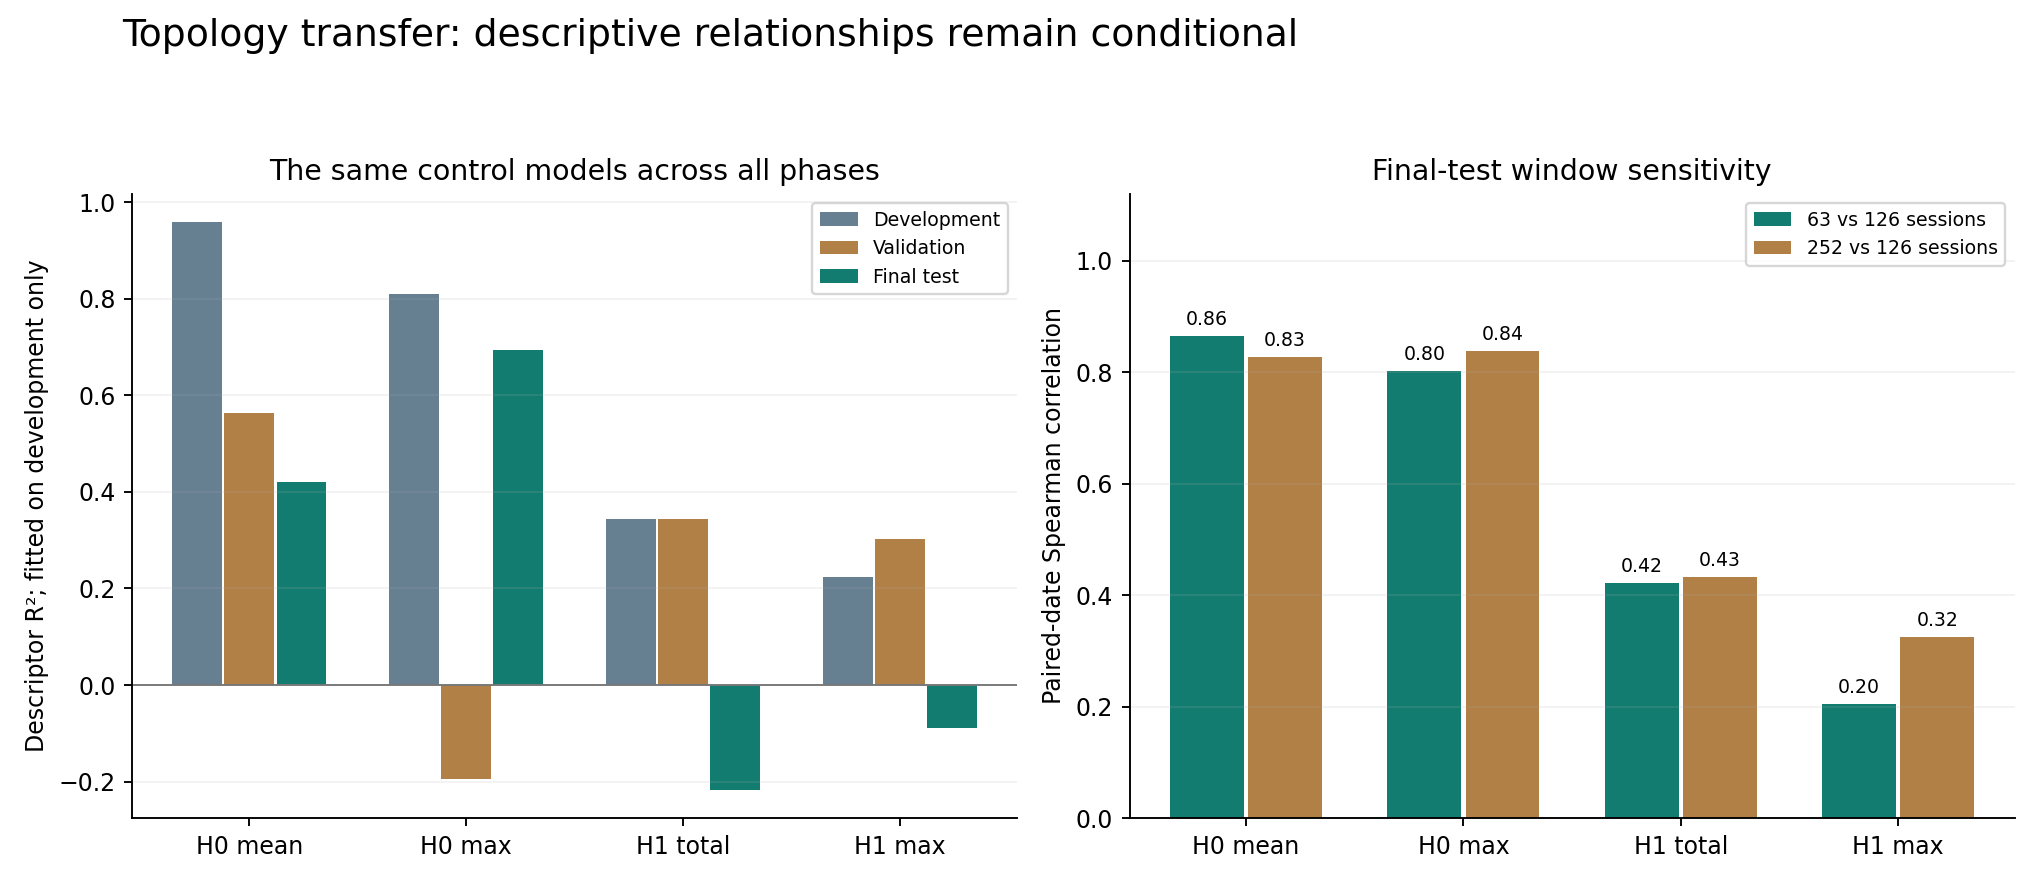
\includegraphics[width=.86\linewidth,height=.65\textheight,keepaspectratio]{assets/figure-16.png}

\caption{Frozen control-model transfer and topology window sensitivity}\label{fig:16}

\end{figure}

All 288 final monthly diagram-bound checks pass. As Chazal et al. (2014) explain in \textit{Persistence stability for geometric complexes}, a metric stability relationship controls diagram changes; it does not imply financial usefulness or horizon-invariant descriptors. The distinction identified in Milestone 4 remains material here.


Following the landscape representation discussed by Bubenik (2015) in \textit{Statistical topological data analysis using persistence landscapes}, the final companion contains 72 monthly 3D landscapes and paired diagrams. Its axes and first-five-layer display convention are fixed across frames. The file {\fontsize{9.3}{12}\selectfont\nolinkurl{outputs/final/topology/Final-Test-Landscape-Explorer.html}} explains observed structure, not a trade recommendation. Numerical frame values and controls are checked; live browser interaction is not claimed as tested in the build environment.


\Needspace{4\baselineskip}\subsection{Research conclusion}

The fixed strategy comparison fails its predefined positive-evidence criterion. The implementation and mathematical checks are completed, but profitability and a reliable incremental graph advantage are not demonstrated in this survivor-basket study. Topology contributes a verified descriptive analysis with explicit redundancy and stability limitations. The reserved period is now observed and cannot be reused as a fresh test for subsequent model changes.


\bodyheading{Setbacks, design forks and their treatment}

The project records methodological forks, observed empirical setbacks and implementation failures separately. A design safeguard is not described as a bug that occurred. The detailed record in {\fontsize{9.3}{12}\selectfont\nolinkurl{docs/milestone-decisions.md}} identifies the evidence, response and unresolved limitation for every completed milestone. The Milestone 1–3 entries are retrospective summaries of retained artifacts; the Milestone 4 and 5 entries were written during their respective work.


\begingroup
\setcounter{table}{25}
\setstretch{1}\fontsize{10}{12.5}\selectfont
\renewcommand{\arraystretch}{1.12}
\arrayrulecolor{tablerule}
\renewcommand{\arraystretch}{1.06}
\setlength{\aboverulesep}{1pt}\setlength{\belowrulesep}{1pt}
\begin{table}[!htbp]
\centering
\setstretch{1}\fontsize{10}{12.5}\selectfont
\begin{tabular}{P{0.170000\dimexpr\textwidth-6\tabcolsep\relax}P{0.350000\dimexpr\textwidth-6\tabcolsep\relax}P{0.480000\dimexpr\textwidth-6\tabcolsep\relax}}
\toprule
\rowcolor{tablehead} \textbf{Milestone} & \textbf{Setback or fork} & \textbf{Response and remaining limit} \\ \midrule
1. Foundations & Synthetic mean reversion favours the intended signal; exposure and timing conventions need explicit decisions & Treat synthetic returns as engine checks; test projection, delayed execution, drift costs and terminal liquidation; real-market usefulness remains untested at this stage \\
\midrule[0.2pt]
2. Historical baseline & Available data omit a point-in-time universe; default-cost returns are negative & Label the survivor-basket scope, preserve source hashes and every fee case; no stock/date substitution; survivorship bias and profitability remain unresolved \\
\midrule[0.2pt]
3. Graph comparison & Equal exposure ceilings yield different actual gross; the apparent validation gain is uncertain & Add declared matched-gross controls and dependent-return intervals; retain the negative development result and confidence interval spanning zero \\
\midrule[0.2pt]
4. Topology & H0 overlaps simple correlation; H1 is window-sensitive; an H0 control relation transfers poorly & Keep simple controls, all windows and negative R\(^{2}\); do not choose a favourable setting or introduce an untested overlay; numerical verification is complete but financial usefulness remains open \\
\midrule[0.2pt]
5. Final evaluation & Default-cost losses persist; paired improvement is uncertain; some topology/control relations fail to transfer; one saved ledger was empty & Lock criteria before acquisition; retain all cases and negative findings; repair output writes and reproduce unaffected hashes; the test is now observed \\
\bottomrule
\end{tabular}
\caption{Problem-solving record across completed milestones}\label{tab:26}
\end{table}
\endgroup

The first final run also exposed a persistence failure: one sensitivity ledger was empty despite a completed in-memory calculation. The original manifest is retained. Verified atomic writes and a full replay repair the artifact, with every unaffected numerical-output hash required to match and every saved ledger checked against its original summary. The exact cause of the original write failure was not established. A separate notebook assertion found stale slider entries left by an array merge in the reused 3D layout. Explicit slider replacement and exact frame/slider calendar checks repaired that defect; live browser interaction remains a separate local check.


The mitigation is not always a successful new model. For the historical losses and unstable feature relationships, the appropriate response is to narrow the claim, preserve the evidence and state the next decision explicitly. As White (2000) explains in \textit{A Reality Check for Data Snooping}, searching many alternatives complicates interpretation; as Bailey et al. (2017) discuss in \textit{The probability of backtest overfitting}, a final holdout alone does not erase that search. The protocol history therefore remains part of the final research narrative.


\bodyheading{Discussion and limitations}

\Needspace{4\baselineskip}\subsection{What the comparison establishes}

The research began with three related questions: whether the baseline survives the declared charges, whether a graph-relative construction improves that baseline, and whether persistent homology adds useful information beyond simpler descriptors. The results answer these questions at different levels. The baseline and graph implementations satisfy their declared numerical constraints, but neither is profitable at the default costs in development, validation or the final test. The graph has a smaller final loss, yet its paired improvement remains uncertain and is reduced by matching gross exposure. Consequently, the evidence does not establish a profitable or reliably superior graph strategy.


The distinction between implementation and economic evidence is central to the result. Dollar neutrality and estimated-beta neutrality are constraints on a portfolio formed from current estimates. They do not guarantee future neutrality, low losses or a positive expected return. As Fama and French (1993) explain in \textit{Common risk factors in the returns on stocks and bonds}, common variation extends beyond a single market factor. The nonzero realised SPY beta and unconstrained sector and other factor exposures therefore remain relevant even when numerical projection errors are negligible.


The cost decomposition identifies the immediate accounting obstacle. In the final test, the graph's annualised arithmetic gross contribution is approximately 1.00\%, while trading and borrowing drag total approximately 5.81\%. The baseline has a smaller gross contribution and slightly greater drag. These observations explain the retained ledger outcomes under the declared assumptions. They do not establish a universally correct brokerage fee, a causal estimate of each market friction or the performance of a different rebalancing rule. A lower-turnover design would constitute a new hypothesis requiring a new experiment.


\Needspace{4\baselineskip}\subsection{What topology establishes}

Persistent homology provides a well-defined description of the rolling correlation geometry. H0 component-merger summaries and H1 cycle lifetimes were computed with explicit filtration and boundary conventions, and independently checked using known shapes and spanning-tree relationships. The descriptors are therefore reproducible mathematical objects within the declared construction.


The scientific interpretation is more limited. H0 mean persistence substantially overlaps ordinary mean correlation. H1 retains variation beyond the specified linear controls, but its ranking changes with the estimation window and some control relationships transfer poorly. As Chazal et al. (2014) explain in \textit{Persistence stability for geometric complexes}, a perturbation bound concerns changes in the underlying metric geometry and the resulting diagrams. Passing that bound does not guarantee a stable economic regime, a transferable fitted model or a profitable use of the descriptors. The decision to retain topology as a diagnostic follows from those distinctions.


\Needspace{4\baselineskip}\subsection{Scope of the data and inference}

The universe is a retrospectively selected basket of surviving companies. Clean calendars and complete adjusted prices do not turn it into a point-in-time investable universe. As Shumway (1997) explains in \textit{The Delisting Bias in CRSP Data}, missing adverse outcomes can affect historical inference. This study does not estimate the size or direction of its own broader selection bias. Its conclusions are conditional on the specified basket and should not be extrapolated to all US equities.


Current-vintage adjusted returns also simplify the relation between observations and executable positions. The separate final vintage passes the declared overlap audit, but that audit is not an independent certification of every historical adjustment. The ledger omits security-specific borrow availability, financing rebates, nonlinear market impact, raw execution prices and a complete corporate-action cash account. These omissions limit deployment interpretation even if the fixed backtest were profitable.


The uncertainty procedures preserve paired dates and model short-range dependence, but they remain approximate and conditional. As Lehmann and Romano (2005) discuss in \textit{Testing Statistical Hypotheses}, controlling an explicit family of comparisons is different from attaching an individual error probability to each claim. The Bonferroni allocation covers the three specified final means subject to adequate marginal coverage. It does not cover an unlimited research history. White (2000), in \textit{A Reality Check for Data Snooping}, and Bailey et al. (2017), in \textit{The probability of backtest overfitting}, provide the broader context for retaining the full sequence of decisions rather than treating the final split as a complete correction for selection.


Finally, the reserved observations are public historical years. The protocol lock establishes the order of work within this project, not prospective blindness to market history. The final data have now been inspected. Reusing those years to choose a revised signal, cost setting or topology threshold would make them part of development, not a new confirmatory test.


\bodyheading{Conclusion and future work}

\Needspace{4\baselineskip}\subsection{Conclusion}

The objective of this project was to develop and evaluate a market-neutral trading framework that uses relationships between stock returns while accounting explicitly for costs and market exposure. The implementation objective was achieved: the completed Python framework integrates a reversal baseline, graph diffusion, constrained portfolio formation, delayed execution, a reconciled cost ledger, dependence-aware uncertainty and persistent-homology diagnostics. The financial objective was not demonstrated. Under the fixed universe and stated costs, the proposed graph strategy does not establish profitable or reliably superior performance.


The final 2020–2025 evaluation is the decisive comparison for the frozen design. At 5 basis points per dollar traded and 2\% annual short borrow, baseline CAGR is \( - \)5.57\% and primary graph CAGR is \( - \)4.80\%. The graph's annualised arithmetic improvement of +0.73 percentage points has an adjusted interval spanning \( - \)2.14 to +3.85 percentage points. Matched-gross results also leave the direction of the improvement unresolved. None of the four necessary evidence conditions specified before final-data acquisition is met. The smaller observed loss must therefore be reported as a descriptive finding, rather than evidence of profitable alpha.


The topology study contributes a separate result. Persistent homology can be computed causally and checked against known mathematical relationships, but additional mathematical structure does not automatically create additional financial value. H0 substantially overlaps a simpler correlation measure, while H1 is sensitive to the estimation horizon and some descriptive models transfer poorly. Retaining those limitations and declining to add an unsupported trading overlay are part of the research outcome.


The project also demonstrates how setbacks can improve the quality of an investigation without changing an unsuccessful hypothesis into a successful one. Exposure differences motivated a matched-gross control; serial dependence motivated paired uncertainty procedures; revised adjusted-price histories motivated a return-overlap audit; and failed output and slider checks motivated verified persistence and explicit interactive-calendar validation. These responses make the analysis more transparent and reproducible. They do not remove the negative economic finding or the limits of the data.


Accordingly, the final contribution is an auditable quantitative research process: established relationships are attributed, project choices are declared, every planned scenario is retained, and conclusions follow the evidence. The combination of mathematical derivation, executable code, diagnostic figures and a documented decision record provides a foundation for further research, while keeping the boundary between engineering correctness and investment performance explicit.


\Needspace{4\baselineskip}\subsection{Future work}

The first priority for a stronger financial study is a point-in-time universe with delisting outcomes, a more complete corporate-action record and historical borrowing information. Those observations would permit a broader assessment of sample validity and implementability. They should be acquired and audited before selecting additional model complexity.


A separate experiment could investigate whether a slower rebalancing schedule or an explicit trading threshold improves the relationship between gross contribution and recurring costs. Such a change must be specified before examining newly reserved observations, with the original baseline retained and the full candidate set reported. The current final period cannot be reused as an untouched test for that choice.


Any future use of topology should begin with a precise economic hypothesis, a stated feature direction and a training-only rule. It should then be compared with ordinary correlation and volatility controls under the same timing, exposure and cost conventions. Persistent-homology computation alone is insufficient justification for a trading overlay.


The remaining presentation work is to publish the reproducible source structure and interactive companions with accurate CV and LinkedIn descriptions. Those descriptions should emphasise implementation, empirical testing, mathematical verification and the retained negative result. A claim of demonstrated profitable alpha would go beyond the evidence established by this project.
\FloatBarrier\clearpage\phantomsection\section*{References}\addcontentsline{toc}{section}{References}
\begingroup\setstretch{1}\fontsize{10.5}{13.5}\selectfont
\refentry{Avellaneda, M. and Lee, J.-H. (2010) ‘Statistical arbitrage in the US equities market’, \textit{Quantitative Finance}, 10(7), pp. 761–782. doi: \href{https://doi.org/10.1080/14697680903124632}{10.1080/14697680903124632}.}

\refentry{Bailey, D.H., Borwein, J.M., Lopez de Prado, M. and Zhu, Q.J. (2017) ‘The probability of backtest overfitting’, \textit{The Journal of Computational Finance}, 20(4), pp. 39–69. doi: \href{https://doi.org/10.21314/JCF.2016.322}{10.21314/JCF.2016.322}.}

\refentry{Bauer, U. (2021) ‘Ripser: efficient computation of Vietoris–Rips persistence barcodes’, \textit{Journal of Applied and Computational Topology}, 5(3), pp. 391–423. doi: \href{https://doi.org/10.1007/s41468-021-00071-5}{10.1007/s41468-021-00071-5}.}

\refentry{Bubenik, P. (2015) ‘Statistical topological data analysis using persistence landscapes’, \textit{Journal of Machine Learning Research}, 16(3), pp. 77–102. Available at: \url{https://jmlr.org/papers/v16/bubenik15a.html} (Accessed: 21 September 2026).}

\refentry{Chazal, F., de Silva, V. and Oudot, S. (2014) ‘Persistence stability for geometric complexes’, \textit{Geometriae Dedicata}, 173(1), pp. 193–214. doi: \href{https://doi.org/10.1007/s10711-013-9937-z}{10.1007/s10711-013-9937-z}.}

\refentry{Chung, F.R.K. (1997) \textit{Spectral Graph Theory}. CBMS Regional Conference Series in Mathematics, 92. American Mathematical Society. doi: \href{https://doi.org/10.1090/cbms/092}{10.1090/cbms/092}.}

\refentry{Edelsbrunner, H., Letscher, D. and Zomorodian, A. (2002) ‘Topological Persistence and Simplification’, \textit{Discrete and Computational Geometry}, 28, pp. 511–533. doi: \href{https://doi.org/10.1007/s00454-002-2885-2}{10.1007/s00454-002-2885-2}.}

\refentry{Fama, E.F. and French, K.R. (1993) ‘Common risk factors in the returns on stocks and bonds’, \textit{Journal of Financial Economics}, 33(1), pp. 3–56. doi: \href{https://doi.org/10.1016/0304-405X(93)90023-5}{10.1016/0304-405X(93)90023-5}.}

\refentry{Gidea, M. and Katz, Y. (2018) ‘Topological data analysis of financial time series: Landscapes of crashes’, \textit{Physica A: Statistical Mechanics and its Applications}, 491, pp. 820–834. doi: \href{https://doi.org/10.1016/j.physa.2017.09.028}{10.1016/j.physa.2017.09.028}.}

\refentry{Golub, G.H. and Van Loan, C.F. (2013) \textit{Matrix Computations}. 4th edn. Johns Hopkins University Press. doi: \href{https://doi.org/10.56021/9781421407944}{10.56021/9781421407944}.}

\refentry{Kondor, R.I. and Lafferty, J.D. (2002) ‘Diffusion Kernels on Graphs and Other Discrete Input Spaces’, in \textit{Proceedings of the 19th International Conference on Machine Learning}, pp. 315–322. doi: \href{https://doi.org/10.5555/645531.655996}{10.5555/645531.655996}.}

\refentry{Lehmann, E.L. and Romano, J.P. (2005) \textit{Testing Statistical Hypotheses}. 3rd edn. Springer Texts in Statistics. Springer. doi: \href{https://doi.org/10.1007/0-387-27605-X}{10.1007/0-387-27605-X}.}

\refentry{Lo, A.W. (2002) ‘The Statistics of Sharpe Ratios’, \textit{Financial Analysts Journal}, 58(4), pp. 36–52. doi: \href{https://doi.org/10.2469/faj.v58.n4.2453}{10.2469/faj.v58.n4.2453}.}

\refentry{Lo, A.W. and MacKinlay, A.C. (1990) ‘When Are Contrarian Profits Due to Stock Market Overreaction?’, \textit{The Review of Financial Studies}, 3(2), pp. 175–205. doi: \href{https://doi.org/10.1093/rfs/3.2.175}{10.1093/rfs/3.2.175}.}

\refentry{Mantegna, R.N. (1999) ‘Hierarchical structure in financial markets’, \textit{The European Physical Journal B}, 11, pp. 193–197. doi: \href{https://doi.org/10.1007/s100510050929}{10.1007/s100510050929}.}

\refentry{Newey, W.K. and West, K.D. (1987) ‘A Simple, Positive Semi-Definite, Heteroskedasticity and Autocorrelation Consistent Covariance Matrix’, \textit{Econometrica}, 55(3), pp. 703–708. doi: \href{https://doi.org/10.2307/1913610}{10.2307/1913610}.}

\refentry{Nordman, D.J. (2009) ‘A note on the stationary bootstrap's variance’, \textit{The Annals of Statistics}, 37(1), pp. 359–370. doi: \href{https://doi.org/10.1214/07-AOS567}{10.1214/07-AOS567}.}

\refentry{Politis, D.N. and Romano, J.P. (1994) ‘The Stationary Bootstrap’, \textit{Journal of the American Statistical Association}, 89(428), pp. 1303–1313. doi: \href{https://doi.org/10.1080/01621459.1994.10476870}{10.1080/01621459.1994.10476870}.}

\refentry{Sharpe, W.F. (1964) ‘Capital Asset Prices: A Theory of Market Equilibrium under Conditions of Risk’, \textit{The Journal of Finance}, 19(3), pp. 425–442. doi: \href{https://doi.org/10.1111/j.1540-6261.1964.tb02865.x}{10.1111/j.1540-6261.1964.tb02865.x}.}

\refentry{Shumway, T. (1997) ‘The Delisting Bias in CRSP Data’, \textit{The Journal of Finance}, 52(1), pp. 327–340. doi: \href{https://doi.org/10.1111/j.1540-6261.1997.tb03818.x}{10.1111/j.1540-6261.1997.tb03818.x}.}

\refentry{Tralie, C., Saul, N. and Bar-On, R. (2018) ‘Ripser.py: A lean persistent homology library for Python’, \textit{Journal of Open Source Software}, 3(29), p. 925. doi: \href{https://doi.org/10.21105/joss.00925}{10.21105/joss.00925}.}

\refentry{White, H. (2000) ‘A Reality Check for Data Snooping’, \textit{Econometrica}, 68(5), pp. 1097–1126. doi: \href{https://doi.org/10.1111/1468-0262.00152}{10.1111/1468-0262.00152}.}

\refentry{Yahoo Finance (2026a) \textit{Historical daily chart responses for the declared stock basket and SPY, 2009–2019}. Available at: \url{https://query1.finance.yahoo.com/v8/finance/chart/SPY?period1=1230768000&period2=1577836800&interval=1d&events=div\%2Csplits} (Accessed: 21 September 2026).}

\refentry{Yahoo Finance (2026b) \textit{Historical daily chart responses for the declared stock basket and SPY, 2018–2025}. Available at: \url{https://query1.finance.yahoo.com/v8/finance/chart/SPY?period1=1546214400&period2=1767225600&interval=1d&events=div\%2Csplits} (Accessed: 22 September 2026).}
\endgroup
\clearpage\appendix\titleformat{\section}{\normalfont\fontsize{15}{18}\bfseries}{Appendix \thesection}{0.7em}{}

\section{Reproducibility and interactive companions}

\begingroup
\setcounter{table}{26}
\setstretch{1}\fontsize{10}{12.5}\selectfont
\renewcommand{\arraystretch}{1.12}
\arrayrulecolor{tablerule}
\begin{table}[!htbp]
\centering
\setstretch{1}\fontsize{10}{12.5}\selectfont
\begin{tabular}{P{0.290000\dimexpr\textwidth-4\tabcolsep\relax}P{0.710000\dimexpr\textwidth-4\tabcolsep\relax}}
\toprule
\rowcolor{tablehead} \textbf{Artifact} & \textbf{Current state} \\ \midrule
Historical inputs & Original cache preserved; separate final-period vintage with 2019 warm-up, hashes and overlap audit \\
\midrule[0.2pt]
Trading comparison & All 44 graph/baseline scenarios retained with uncertainty and exposure controls \\
\midrule[0.2pt]
Topology & Four features, three windows, complete control comparisons, fitted coefficients and monthly diagrams \\
\midrule[0.2pt]
Interactive companions & Historical correlation surface, graph/score explorer and earlier/final-period persistence landscapes \\
\midrule[0.2pt]
Walkthroughs & Five notebooks; final evaluation executed with captured outputs \\
\midrule[0.2pt]
Scientific text & Current manuscript uses Harvard author–date citations and an alphabetical reference list \\
\midrule[0.2pt]
Engineering verification & 41 automated checks; 480 earlier and 288 final-period diagram bounds; artifact and causal checks \\
\midrule[0.2pt]
Final test & 2020–2025 released after a new protocol lock; all 22 cases completed; now observed \\
\midrule[0.2pt]
Public release & Reproducible source structure and CI prepared; GitHub/LinkedIn publication remains a later deliverable \\
\bottomrule
\end{tabular}
\caption{Research artifacts and reproduction status}\label{tab:27}
\end{table}
\endgroup

Run {\ttfamily\fontsize{11.5}{13}\selectfont python run\_final.py} for the complete final experiment after installing the pinned dependencies. {\ttfamily\fontsize{11.5}{13}\selectfont python -m unittest discover -s tests -v} runs the focused checks. The private research ZIP includes the acquired observations for exact offline replay. An eventual public checkout will exclude vendor caches because redistribution rights cannot be assumed. A fresh acquisition may have a different data vintage and requires a documented revision rather than a bypass of the input hash guard.


The editable manuscript is assembled by {\ttfamily\fontsize{11.5}{13}\selectfont python paper/update\_manuscript.py} from section files, implementation excerpts, result tables and the source register. {\ttfamily\fontsize{11.5}{13}\selectfont python paper/assemble\_final\_paper.py} prepares the portrait typesetting source, copies the declared figures and compiles the final PDF. The accompanying source package includes a standalone LaTeX file and its figure assets. Caption registers and page references are generated from the compiled document.


\Needspace{4\baselineskip}\subsection{Interactive companions}

The historical-correlation companion displays 120 monthly matrices. The graph-diffusion companion links 120 monthly networks to unconstrained scores. The earlier persistence companion displays 120 monthly landscapes and birth–death diagrams; the final-period companion adds 72 months covering 2020–2025. Each HTML file embeds its plotting library for offline use after download. Rotation, date selection, hover and playback support inspection of the underlying numerical objects. The PDF contains static figures; the HTML files provide the dynamic views.


Numerical frame values, dates and control configuration were checked. Live browser interaction and local VS Code kernel connectivity were not exercised in the build environment and remain local setup checks. These limits concern the execution environment, whereas the saved numerical results and notebook cells were executed and verified.


\Needspace{4\baselineskip}\subsection{Publication status and future changes}

The scientific evaluation and final paper are complete for the frozen design. Public GitHub publication and the CV/LinkedIn release are subsequent presentation steps. Claims should describe the implemented methods, verification and empirical findings, including the negative economic result. The evidence does not support a claim of demonstrated profitable alpha. All three research periods are observed; future model changes need newly reserved evidence.


\Needspace{4\baselineskip}\subsection{Final document assembly}

The final assembly follows the author's supplied style examples while retaining the research sequence developed for this project. All pages use A4 portrait dimensions, with numbered equations and centred captions below figures, tables and equations. The build generates the contents and caption registers from the typeset document. Initial checks exposed sparse front-matter continuations and caption-box and font issues; compact register tables, explicit font selection and revised caption placement resolved them. Rendered-page inspection and position checks verify presentation separately from the numerical research. This assembly is recorded in the sixth milestone's decision log; public publication remains pending.

\end{document}
